\documentclass{report}
\usepackage{graphicx} % Required for inserting images
\usepackage{xcolor}
\usepackage{biblatex} %Imports biblatex package
\usepackage{A4}
\usepackage{array}
\usepackage{float}
\usepackage{amsmath}
\usepackage{todonotes}
\usepackage{multirow}
% \usepackage{subcaption}

\usepackage{subfig}
\newcommand{\gna}[1]{\todo[color=yellow!20,inline]{Ghassen: #1}}
\newcommand{\rpa}[1]{\todo[color=blue!20,inline]{Rashmi: #1}}
\newcommand{\ate}[1]{\todo[color=red!20,inline]{Armin: #1}}



\addbibresource{BiGER_bibliography.bib} %Import the bibliography file

\title{BiGER project: Implementations Report}
\author{Rashmi Prasad$^1$, Ghassen Nakti, Armin Teskeredžić, Thierry Van Cutsem, Mathilde Bongrain, \\
$^1$ supervision at TU Delft: Aleksandra Lekić and Pedro P. Vergara}
\date{June 2024}

\begin{document}

\maketitle


\section*{Introduction}
The first objective of the project was to conduct an extensive literature review about the state-of-the-art RMS and EMT simulations and their limitations in the stability analysis of power systems. The findings were reported in the first report “State-of-the-art”.
The second objective is to identify and implement a set of relevant benchmark use cases. First, the use case selection will enable to explore and exhibit the reported limitations by demonstrating some of the findings from literature. Second the use cases will prepare the framework for benchmarking alternative solutions in the next project.

The present document "Use Cases Report" summarizes the development process of use cases showing a significant discrepancy between RMS and EMT simulations. For this purpose, the selected test models and test systems forming the use cases are described along with their implementation and validation in RMS and EMT simulators. Understanding the modeling differences helps engineers choose the appropriate tool depending on the specific stability analysis requirements and the nature of the power system phenomena they need to simulate.

\subsection*{Tools selection}
Before starting the implementation process an appropriate selection of power system simulators needs to be made. At least one RMS and one EMT simulator are selected to implement the relevant use cases and compare them to each other. The priority is given to open-source tools when available.
The major challenge when working with simulators is the identification of limitations from physically-driven model behavior vs numerically-driven solver behavior.
Motivated by the open-source requirement and the separation between models and solvers, the following simulators were selected:

\begin{itemize}
    \item \textbf{STEPSS \cite{STEPSS}:} STATIC AND TRANSIENT ELECTRIC POWER SYSTEMS SIMULATION: open-source RMS tool (Univ. of Liège by Prof. T. Van Cutsem)
    \begin{itemize}
        \item Strict separation between modeling and solving parts
        \item Equation-based modeling using a proprietary language
        \item Available collection of relevant converter test models, test systems and test cases
        \item Modules: PFC (for power flow computations), RAMSES (the solverof differential-algebraic equations), and CODEGEN (a tool to develop models).
        \item Designed for steady-state and stability analysis with enhanced modeling capabilities for large-scale power systems.
    \end{itemize}

    \item \textbf{Dynawo \cite{DYNAWO}:} open-source hybrid C++/Modelica RMS tool (RTE)
    \begin{itemize}
        \item Strict separation between modeling and solving parts
        \item Equation-based modelling with high-level modeling language Modelica
        \item Third party advanced open-source solvers
        \item Five modules: DynaFlow for steady-state calculations, DySym for short-circuit calculations, DynaWaltz for long-term stability simulations, DynaSwing for short-term stability studies and DynaWave for stability studies and system design with a high-penetration of power-electronics based components (quasi-EMT).
        \item Three solvers: BE fixed time-step solver(based on research work done during the European project Pegase), trapezoidal fixed time-step solver internally developed and making use of the Krylov Inexact Newton SOLver (KINSOL) algebraic solver, variable time-step solver based on IDA, which is part of SUite of Nonlinear and DIfferential/ALgebraic equation Solvers (SUNDIALS).
    \end{itemize}
    
    \item \textbf{EMTP-RV \cite{EMTP}:}  EMT tool (EDF, Hydro-Québec and RTE)
    \begin{itemize}
        \item Based on nodal analysis/ resistive companion (Dommel's approach)
        \item Widely used by industry and academia
        \item Possibility to access and understand the code in collaboration with EMTP developers from RTE.
        \item Solver is based on assembling network equations based on sparse modified-augmented-nodal analysis. In addition, Jacobian based nonlinear solver eliminates topological restrictions and allows solving very large scale nonlinear systems with a minimized number of iterations.
        \item Known for its detailed and high-fidelity transient analysis. It can simulate fast electromagnetic transients with high accuracy.
    \end{itemize}
\end{itemize}

\subsection*{Test models, test systems and studies}
In this report the selection and implementation of test models; test systems and studies are covered in details. A graphical overview of models, systems, studies and simulators is shown in Figure \ref{fig:Overview}. For a better understanding the chosen terminology in the project is explained below.

\textbf{Test Models}: these are component models of electrical power systems that represent the various elements that make up the entire power network. Each component model simulates the behaviour and characteristics of a specific part of the power system. The focus in the present work is on grid-following Voltage Source Converters (VSCs), and synchronous generators. These test models are used in power system simulation software to analyse the performance, stability, and reliability of electrical power systems under various operating conditions and scenarios. The chosen test models are implemented and validated within the Dynawo and EMTP simulation environments.

\textbf{Test Systems}: the test systems represent the entire network behaviour and interactions, combining various test models into a comprehensive network. Test systems are examples of networks to simulate the performance, stability, and dynamics of the power system under different conditions. The implementation task involved a range of systems including a 1-VSC system, a 4-VSC system, and the Nordic system. Similarly, the selected test systems undergo implementation and validation in both Dynawo and EMTP.

\textbf{Studies}: The studies are dynamic simulation stability analyses scenarios conducted to investigate the ability of the power system to maintain continuous operation under normal and disturbed conditions. The studies relate to the assessment of different types of stability, including rotor angle stability using the critical clearing time (CCT) as metric and small-signal stability to evaluate the system's ability to maintain synchronism under small disturbances focusing on the system's damping of oscillations over time. A study can be also conducted to find the limit of a specific variable or parameter e.g. the effect of external network strength, particularly short circuit power (SCP) on stability. The stability assessment in this case is extended to generic stability metrics such as the system's ability to remain synchronized and maintain voltage and frequency within acceptable limits. In this report, a study to find the limit of external network strength is conducted with the 4-VSC system. The Nordic System is used to investigate the impact of varying penetration levels of VSCs on the critical clearing time. The findings from these studies provide insights into the differences between RMS and EMT dynamic simulations for stability assessments.
\begin{figure}[h]
    \centering
    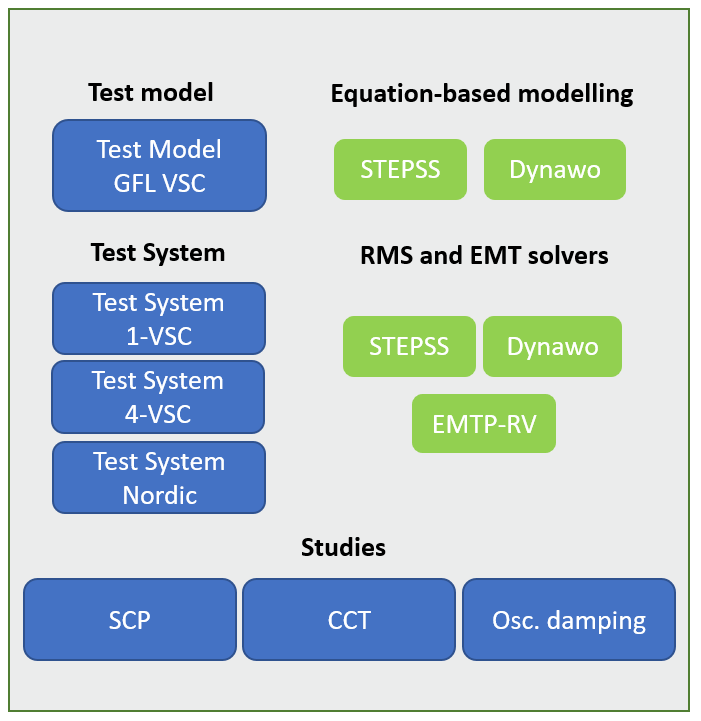
\includegraphics[width=0.8\linewidth]{Overview.PNG}
    \caption{Modelling and simulation overview}
    \label{fig:Overview}
\end{figure}

\chapter{1-VSC test system}
The first stage of benchmarking use cases is the use of a single converter infinite bus case to validate the developed test models, such that an accurate comparison between RMS and EMT simulators can be made. The validation stage proves that the model performs in the way it is designed. It also help to identify any simulator related limitations. This way, the engineer understands the model’s characteristics, its limitations and gains confidence for subsequent studies involving larger networks. The 1-VSC test system has a simple topology, which makes it easy to identify the causes of bugs and gaps. As shown in the single line diagram \ref{fig:1VSC-SLD}, it is composed of a voltage source converter, a transmission line an external network with impedance. The test model is marked with a blue square. 

\begin{figure}[h]
    \centering
    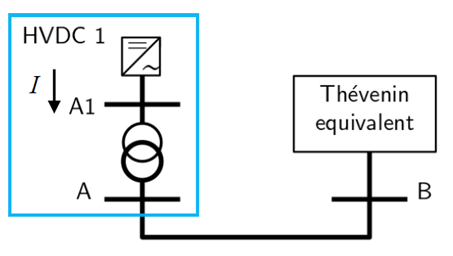
\includegraphics[width=0.5\linewidth]{Figure_1VSC/1VSC.png}
    \caption{1-VSC test system}
    \label{fig:1VSC-SLD}
\end{figure}

In this section, we describe first the selected VSC test model. We present the implementation procedure of the test model and corresponding 1-VSC test system in the different simulators. Finally, we show the results of the model validation.

\section{VSC test model}
The test model selected is a generic grid following inverter model. The motivation behind this selection is the missing of such a generic model in the Dynawo library. The library contains a generic grid forming model and the WECC and IEC standard grid following Wind and PV models. In addition the selection is motivated by the requirement to have the exact same model implemented the different simulators. This will allow for a consistent comparison by excluding discrepancies related to model differences. The selected model is already available in STEPSS.
\\
In the following figure, the VSC model converter connected to the grid through a transformer is presented. The converter operates in grid-following mode, and the DC side is not modelled. Therefore, $v_{dc}$ is assumed constant, and the focus is on the AC grid dynamics.
\begin{figure}[H]
    \centering
    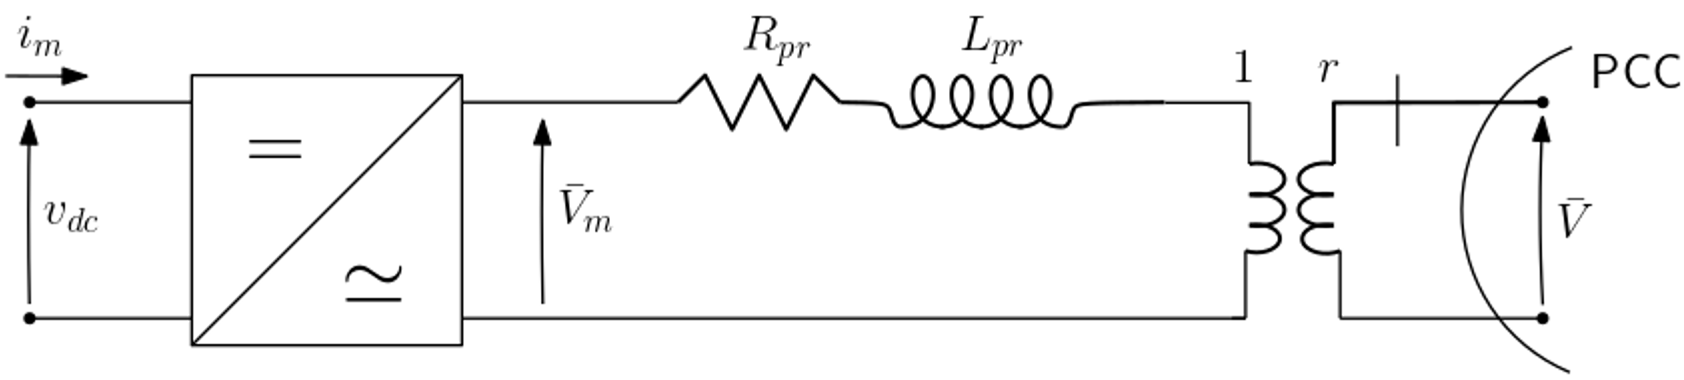
\includegraphics[scale = 0.3]{Figure_converter/converter_model.png}
    \caption{Converter model connected to the grid}
    \label{fig:converter_model}
\end{figure}
Also, no LC filter is used, and the transformer windings R and L are on the primary side.
\\
The DQ0 transformation is used, representing a mathematical technique used in the analysis and control of three-phase electrical systems. It converts three-phase time-domain signals into two stationary (direct and quadrature) components, and one zero-sequence component. The DQ0 transformation consists of the Park and Clarke transformation matrices, where the Clark transform converts vector in the ABC reference frame to the $\alpha\beta\gamma$ (also called XYZ) reference frame. The power-invariant, right-handed, uniformly-scaled Clarke transformation matrix is:
\begin{equation}
    K_C = \sqrt{\frac{2}{3}} 
        \begin{bmatrix}
            1 && -\frac{1}{2} && -\frac{1}{2} \\
            0 && \frac{\sqrt{3}}{2} && -\frac{\sqrt{3}}{2} \\
            \frac{1}{\sqrt{2}} && \frac{1}{\sqrt{2}} && \frac{1}{\sqrt{2}}
        \end{bmatrix}
\end{equation}
The Park transformation converts vectors in the XYZ reference frame to the DQ0 reference frame. Its primary value is to rotate a vector`s reference frame at an arbitrary frequency, and the Park transformation matrix is:
\begin{equation}
    K_P =  
        \begin{bmatrix}
            \cos(\theta) && \sin(\theta) && 0 \\
            -\sin(\theta) && \cos(\theta) && 0 \\
            0 && 0 && 1
        \end{bmatrix}
\end{equation}
Where theta is the instantaneous angle of an arbitrary omega frequency. Together, these two transformation form the DQ0 transformation:
\begin{equation}
\begin{aligned}
    K_{CP} = K_P\cdot K_C &=
    \begin{bmatrix}
            \cos(\theta) && \sin(\theta) && 0 \\
            -\sin(\theta) && \cos(\theta) && 0 \\
            0 && 0 && 1
        \end{bmatrix}
    \cdot
    \sqrt{\frac{2}{3}}
    \begin{bmatrix}
            1 && -\frac{1}{2} && -\frac{1}{2} \\
            0 && \frac{\sqrt{3}}{2} && -\frac{\sqrt{3}}{2} \\
            \frac{1}{\sqrt{2}} && \frac{1}{\sqrt{2}} && \frac{1}{\sqrt{2}}
        \end{bmatrix}
    \\ &=
    \sqrt{\frac{2}{3}}
    \begin{bmatrix}
        \cos(\theta) && \cos(\theta - \frac{2\pi}{3}) && \cos(\theta + \frac{2\pi}{3}) \\
        -\sin(\theta) && -\sin(\theta - \frac{2\pi}{3}) && -\sin(\theta + \frac{2\pi}{3}) \\
        \frac{\sqrt{2}}{2} && \frac{\sqrt{2}}{2} && \frac{\sqrt{2}}{2}
    \end{bmatrix}
\end{aligned}
\label{dq0_equation}
\end{equation}
The reference frames are shown in the next figure, where the network reference frame is represented by (x, y) axes which rotate at angular speed $\omega_{ref}$ (rad/s). The rectangular components of PCC voltage phasor $\bar{V}$ are represented by $v_x$ and $v_y$.
\begin{figure}[H]
    \centering
    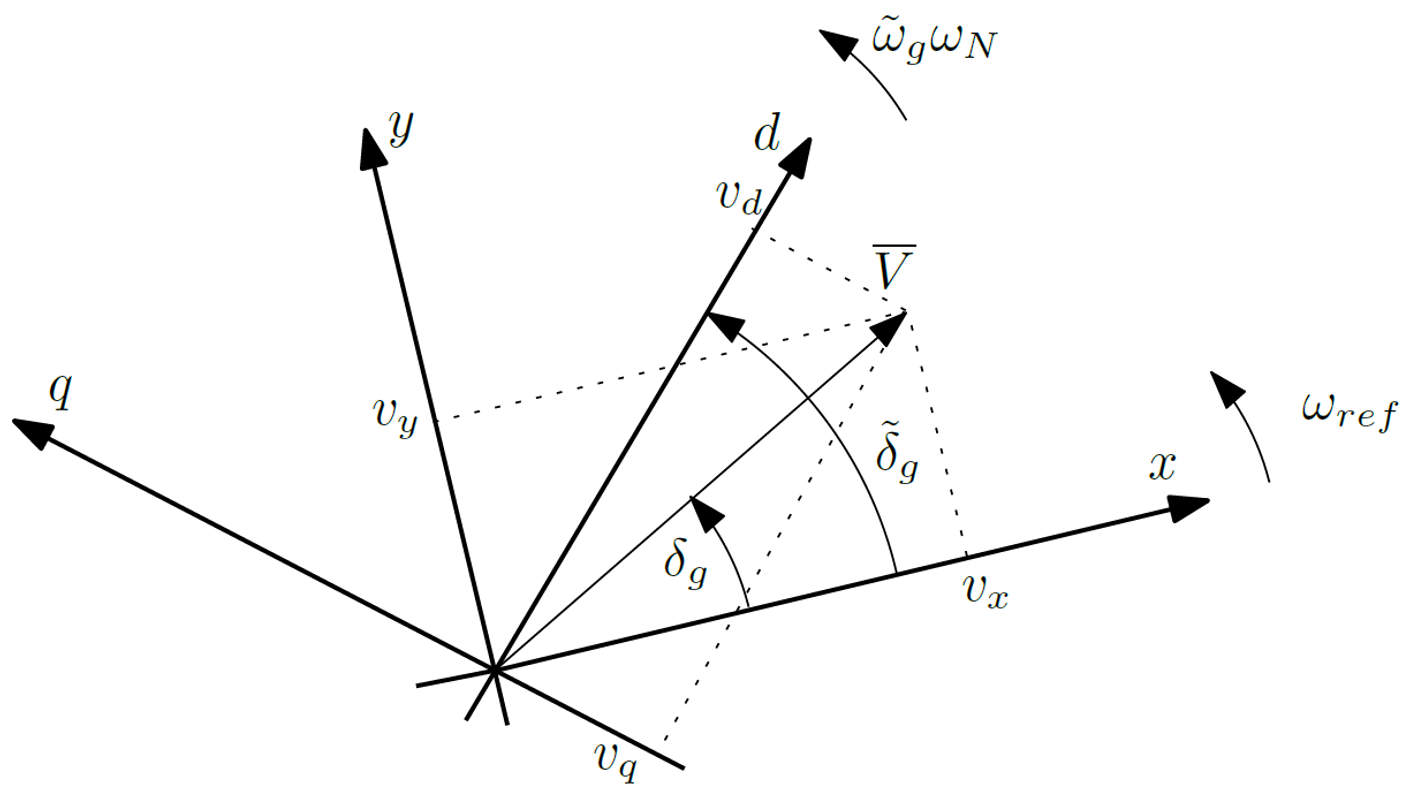
\includegraphics[scale = 0.24]{Figure_converter/reference_frame.png}
    \caption{Reference frames}
    \label{fig:reference_frames}
\end{figure}
where $\omega_N = 2\pi f_n$ is the nominal angular frequency in rad/s. For the VSC control reference frame, the (d, q) axes track the voltage phasor given by the Phase Locked Loop, and $v_d$ and $v_q$ represent the dq components of  $\bar{V}$. The phase angle of $\bar{V}$ is $\delta_g$ in rad, and $\tilde{\omega}_g$ represents the angular speed of (d, q) axes in p.u.. The angle between d and x in rad is denoted as $\tilde{\delta}_g$, where in steady-state $\tilde{\delta}_g = \delta_g$.
\begin{figure}[H]
    \centering
    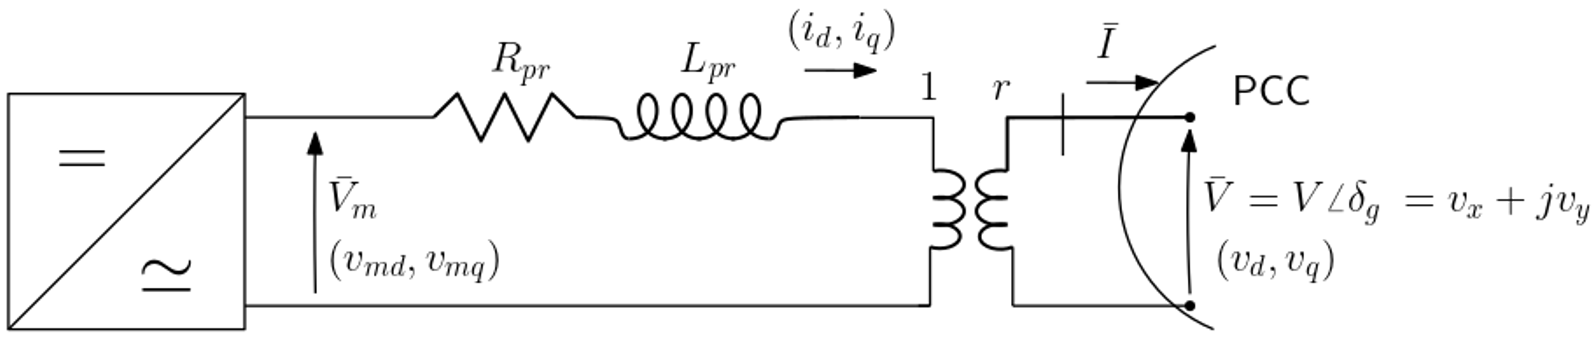
\includegraphics[scale = 0.35]{Figure_converter/converter_model_2.png}
    \caption{Converter model - quantities}
    \label{fig:converter_model_2}
\end{figure}
Passing from (x, y) to (d, q) reference frame, the voltage at PCC is:
\begin{equation}
    v_d = v_x\cos(\tilde{\delta}_g) + v_y\sin(\tilde{\delta}_g),
\end{equation}
\begin{equation}
    v_q = -v_x\sin(\tilde{\delta}_g) + v_y\cos(\tilde{\delta}_g),
\end{equation}
and the current in converter:
\begin{equation}
    i_d = ri_x\cos(\tilde{\delta}_g) + ri_y\sin(\tilde{\delta}_g),
\end{equation}
\begin{equation}
    i_d = -ri_x\sin(\tilde{\delta}_g) + ri_y\cos(\tilde{\delta}_g)
\end{equation}
Dynamics of current in transformer in (d, q) reference frame are given with:
\begin{equation}
    L_{pr}\frac{\text{d}}{\text{d}t}i_d = \omega_N (v_{md} - \frac{v_d}{r} - R_{pr}i_d + \tilde{\omega}_gL_{pr}i_q),
\end{equation}
\begin{equation}
    L_{pr}\frac{\text{d}}{\text{d}t}i_q = \omega_N (v_{mq} - \frac{v_q}{r} - R_{pr}i_q + \tilde{\omega}_gL_{pr}i_d).
\end{equation}
The PLL used in this model has the following diagram:
\begin{figure}[h]
    \centering
    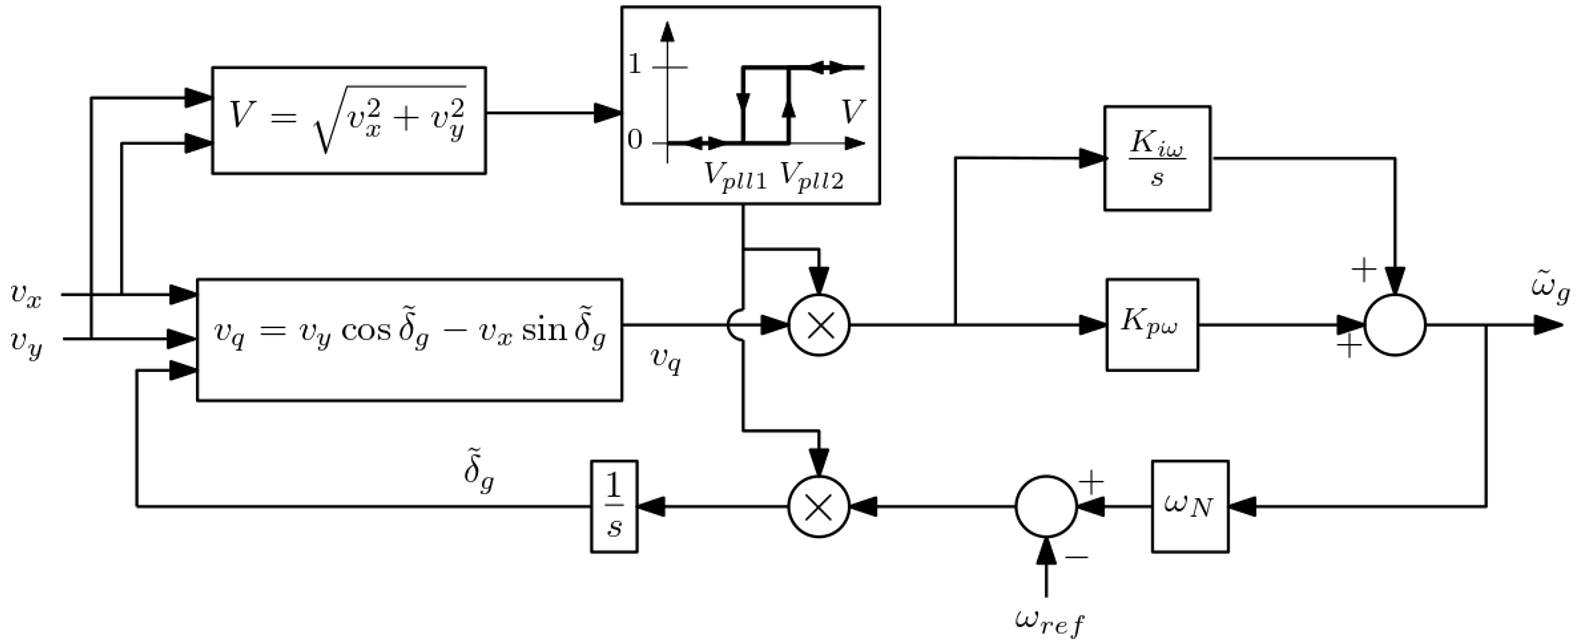
\includegraphics[scale = 0.3]{Figure_converter/PLL.png}
    \caption{PLL block diagram.}
    \label{fig:PLL}
\end{figure}
The gain values are given as:
\begin{equation}
    K_{p\omega} = \frac{10}{T_{pll}\omega_N},
\end{equation}
\begin{equation}
    K_{i\omega} = \frac{25}{T_{pll}^2\omega_N},
\end{equation}
and $T_{pll}$ is the constant of the PLL in s, and has a typical value of 100 ms. It is important to mention, that all other values are in per unit, regarding the $S_{nom}$ base (nominal apparent power of converter). Also, the PLL can be blocked or unblocked for low voltages. That is done by defining $V_{pll1}$ and $V_{pll2}$, which have typical values of 0.4 p.u. and 0.5 p.u., respectively.
\\
The DQ current control is shown in the next figure:
\begin{figure}[H]
    \centering
    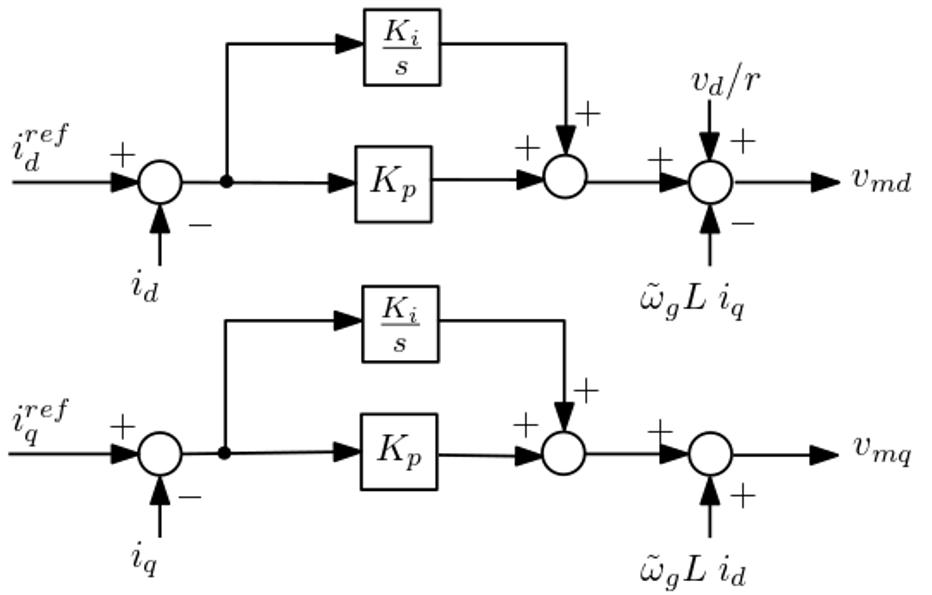
\includegraphics[scale = 0.28]{Figure_converter/DQ_current_control.png}
    \caption{Current control.}
    \label{fig:current_control}
\end{figure}
Where $\omega_c$ equals to 1200 rad/s. The values of the gains are:
\begin{itemize}
    \item $K_i = R_{pr}\omega_c = 6 pu/s$
    \item $K_p = L_{pr} \frac{\omega_c}{\omega_N}$, and it equals to 0.4584 for WP1 and WP2, and 0.5730 for HVDC1 and HVDC2.
\end{itemize}
~\\
The block diagram of the active power control is:
\begin{figure}[H]
    \centering
    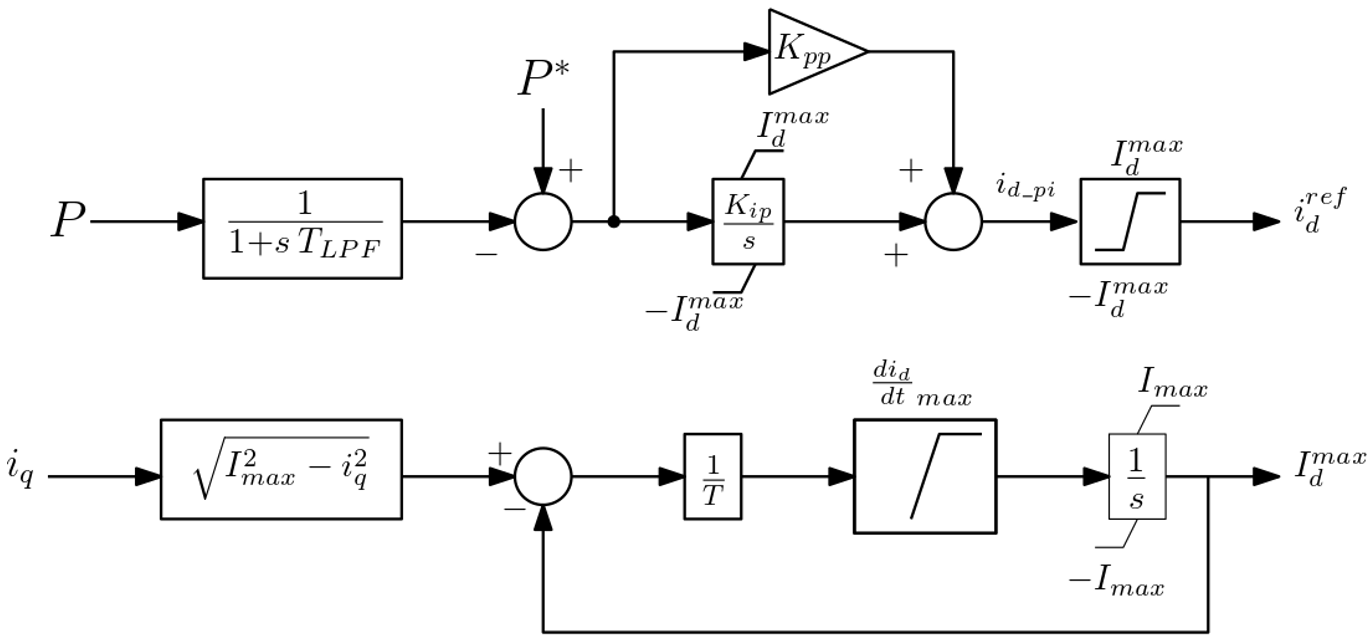
\includegraphics[scale = 0.4]{Figure_converter/active_power_control.png}
    \caption{Active power control.}
    \label{fig:active_power_control}
\end{figure}
The parameters are given as:
\begin{itemize}
    \item $T_{LPF} = \frac{1}{\omega_{LPF}} = \frac{1}{300} = 3.3 ms$
    \item $K_{ip} = 10 pu/s$
    \item $K_{pp} = \frac{K_{ip}}{\omega_{LPF}} = \frac{10}{300} = 0.0333$
\end{itemize}
The second (lower) block in \figurename~\ref{fig:active_power_control} is used to limit the rate of recovery of $I_d^{max}$ after it has been decreased by an increase of $i_q$, since the priority is given to the reactive current. $T$ represents the small time constant in s, and it is equal to 0.002s. The value $(\frac{\text{d}i_d}{\text{d}t})_{max}$ depends on the type of generator. In case for the WP1 and WP2, $(\frac{\text{d}i_d}{\text{d}t})_{max}$ equals to 0.5 pu/s, and for the HVDC1 and HVDC2 $(\frac{\text{d}i_d}{\text{d}t})_{max}$ equals to 10 pu/s.
\\
The block diagram for the reactive power control is shown in the following figure:
\begin{figure}[H]
    \centering
    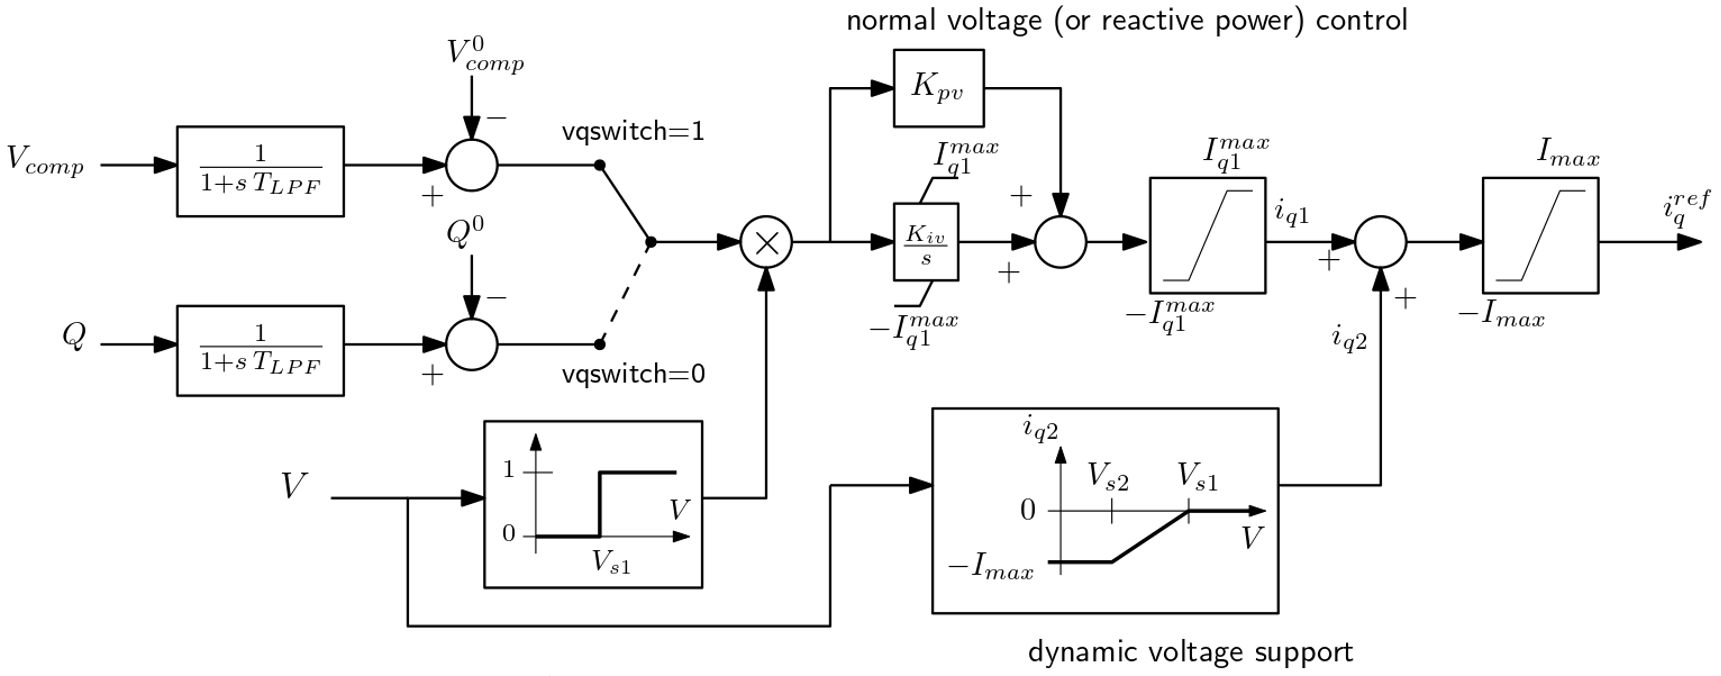
\includegraphics[scale = 0.3]{Figure_converter/reactive_power_control.png}
    \caption{Reactive power control.}
    \label{fig:reactive_power_control}
\end{figure}
The vqswitch must be set to 1 to be in voltage control mode, and we get reactive power control if we set it to 0. The lower block diagram is the voltage support, but in our case it is not considered and that can be achieved by setting $i_{q2}$ = 0.
The parameters and variables are:
\begin{itemize}
    \item Q - reactive power injected into the grid in p.u.
    \item vqswitch - switch used to select voltage or reactive power control
    \item $T_{LPF}$ - time constant of LP filter in s
    \item $V_{comp}$ - compensated voltage $V_{comp} = |\frac{\bar{V}}{r} + (R_c + jX_c)r\bar{I}|$
    \item $R_c = R_{pr}$ and $X_c = L_{pr} \Rightarrow$ the $V_m$ voltage magnitude is controlled
\end{itemize}
The values of $K_{iv}$ and $K_{pv}$ depend on the vqswitch:
\begin{gather*}
    vqswitch = 1:~~~~K_{iv} = 50 pu/s~~~~~K_{pv} = K_{iv}/\omega_{LPF} = 0.1667\\
    vqswitch = 0:~~~~K_{iv} = 10 pu/s~~~~~K_{pv} = K_{iv}/\omega_{LPF} = 0.0333
\end{gather*}
It is also important to limit the current, and that can be explained by the following scheme:
\begin{figure}[H]
    \centering
    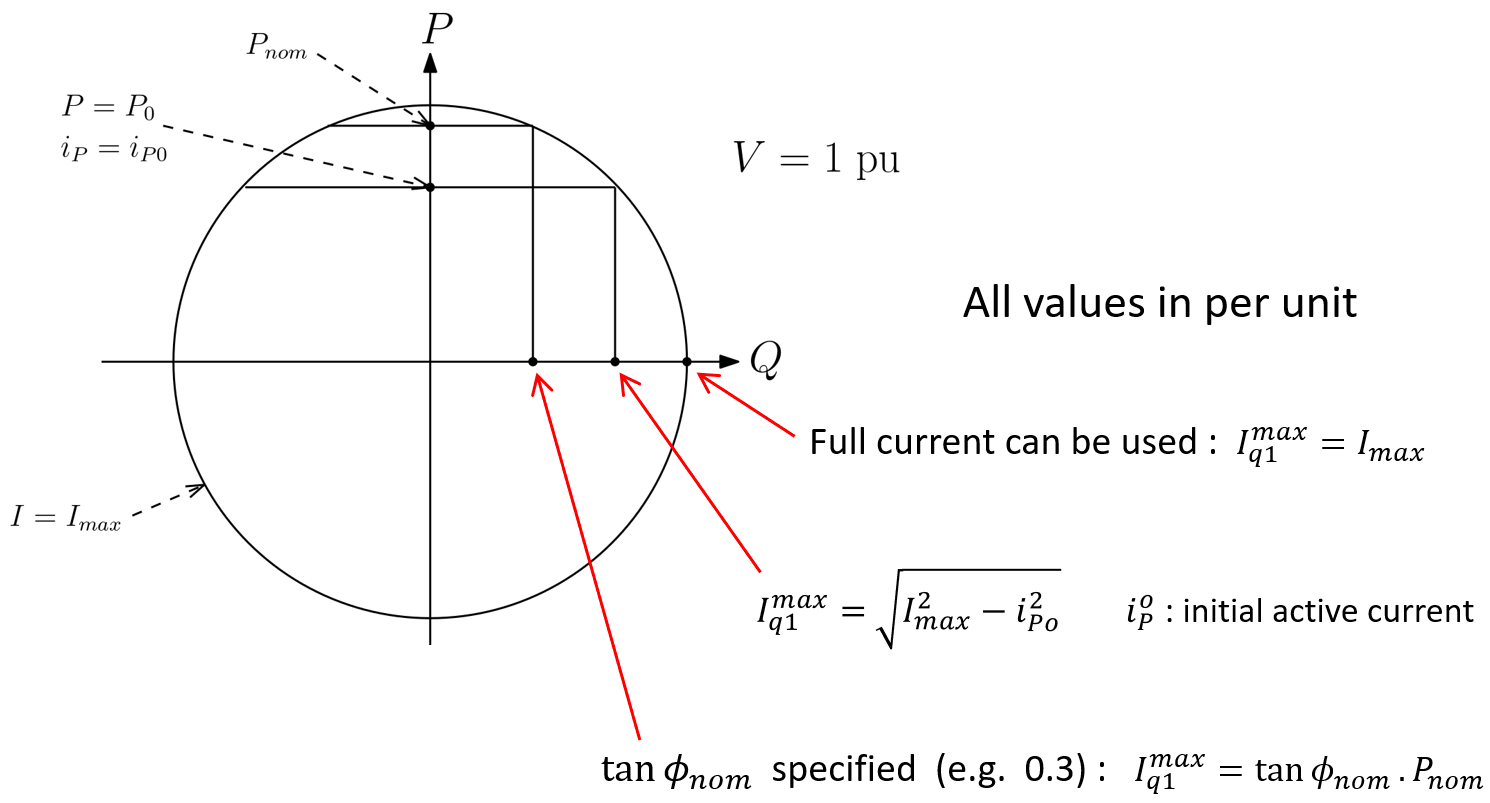
\includegraphics[scale = 0.4]{Figure_converter/current_limit.png}
    \caption{Current limit}
    \label{fig:current_limit}
\end{figure}
There are different modes which can be selected. The first one is when the full reactive current is used $I_{q1}^{max} = I_{max}$. The second one is when the reactive current is limited by the initial current in the converter $I_{q1}^{max} = \sqrt{I_{max}^2 - i_{P0}^2}$, where $i_{P0}^2$ stands for the initial current. The third mode selects the ratio between the reactive current and the nominal power to a specific value: $I_{q1}^{max} = \tan\phi_{nom}\cdot P_{nom}$.

\section{Implementations and validation results}
\subsection{Modelica implementation}
The above described test model is already available in STEPSS along with a suitable 1-VSC system configuration. In the scope of the project, the first task was to develop the same test model and 1-VSC test system in Modelica and integrate them in the open source Dynawo/Modelica library. For this purpose the modeling and simulation environment OpenModelica was used.
Modelica is a high-level modeling language designed for multi-physical systems. It supports object-oriented, declarative programming. It allows the easy formulation of physical laws by mathematical equations (e.g. from literature or other equation-based modelling tools). In addition, with the OpenModelica use interface new components can be modelled as blocks and connected together, which facilitates the implementation of structurally complex systems.

The test model can be divided into two main parts:
\begin{enumerate}
\item The grid following control, which is composed of following elementary blocks:
\begin{itemize}
    \item PLL
    \item Inner current loop
    \item Active power loop (incl. Active current limiter)
    \item Reactive power loop (incl. Reactive current limiter)
\end{itemize}
\item The injector (grid interface), which is composed of the following network components:
\begin{itemize}
    \item Controlled voltage source
    \item Step-up transformer
\end{itemize}
\end{enumerate}

Since no generic grid following VSC model was available in Modelica, all the blocks of the STEPSS model were implemented from scratch. The overall structure of the control is shown in \ref{fig:GFLcontrol_Modelica} and the injector equations in Figure \ref{fig:InjectorGFL_equations_Modelica}.

\begin{figure}[H]
    \centering
    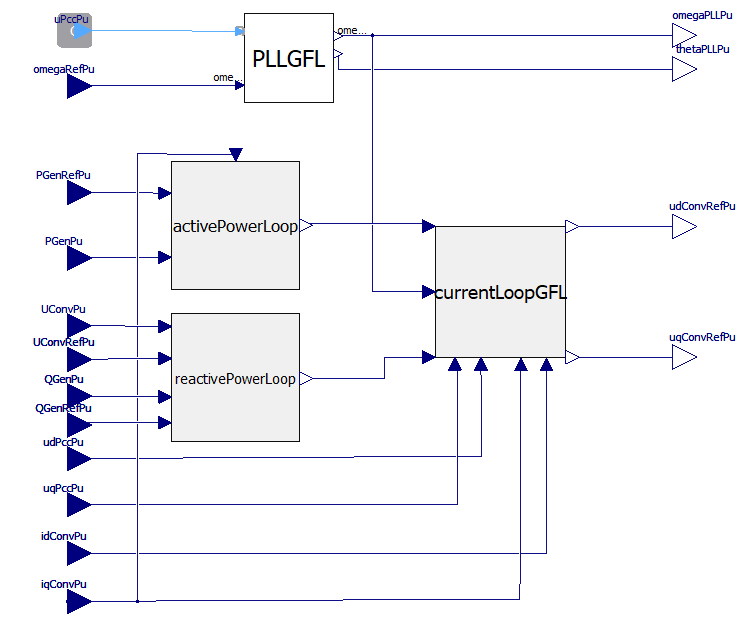
\includegraphics[scale = 0.4]{Figure_1VSC/GFLcontrol_Modelica.PNG}
    \caption{Grid following control structure (OpenModelica)}
    \label{fig:GFLcontrol_Modelica}
\end{figure}

\begin{figure}[H]
    \centering
    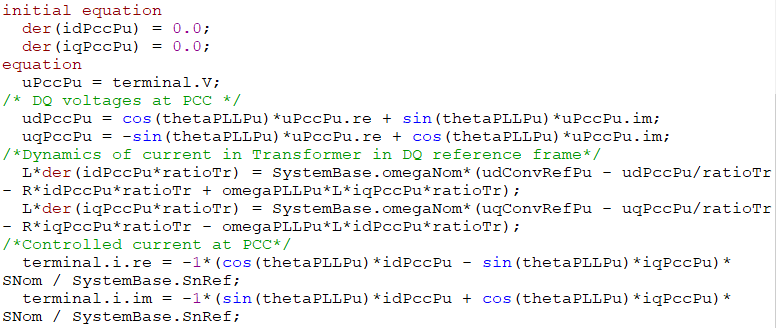
\includegraphics[scale = 0.5]{Figure_1VSC/InjectorGFL_equations_Modelica.PNG}
    \caption{Injector equations (OpenModelica)}
    \label{fig:InjectorGFL_equations_Modelica}
\end{figure}

 Furthermore, the  grid following VSC was test in the 1-VSC test system configuration for validation as shown below:

\begin{figure}[H]
    \centering
    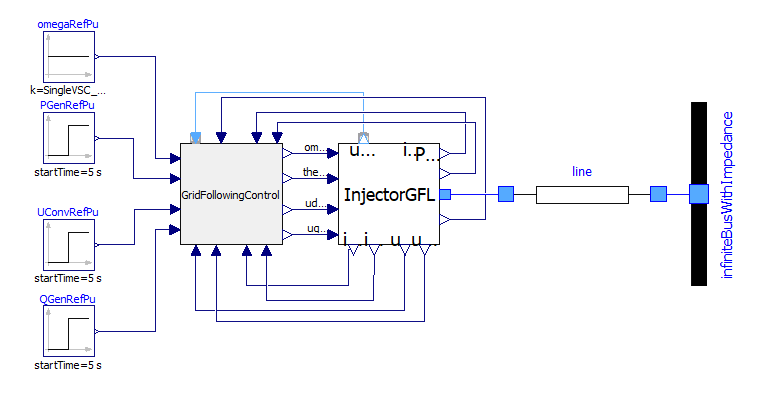
\includegraphics[scale = 0.5]{Figure_1VSC/1VSC_Modelica.PNG}
    \caption{1-VSC test system implementation (OpenModelica)}
    \label{fig:1VSC_Modelica}
\end{figure}


\subsection{Dynawo implementation}
The separation between models and solvers is one of the main characteristics of Dynawo. Dynawo relies for the modelling part on a Dynawo Modelica library. Components can be imported from the library, assembled, and compiled to create a Dynawo model that is then used for a system simulation. For the solution part, Dynawo relies on proprietary and third-party solvers.
In order to assemble the Modelica model in the Dynawo C++ environment and compile it successfully, additional Modelica files are required for specific blocks/ classes:

\begin{enumerate}
    \item Initialisation files: these are Modelica classes files (.mo) with the name ending "INIT" which are required for the upper classes, in this case the grid following control and the injector class. These files contain the parameters, the variables and the equations necessary to initialise the overall model. An example is shown in the following figure:
    \begin{figure}[H]
    \centering
    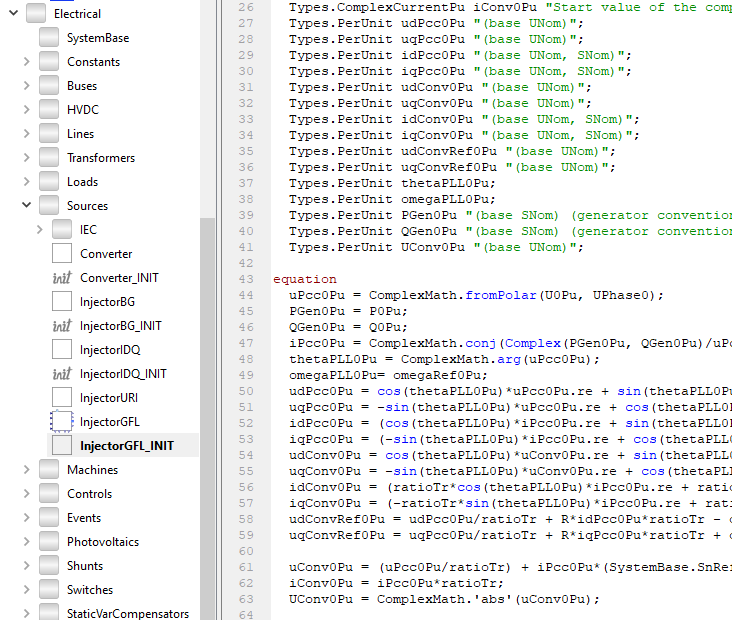
\includegraphics[scale = 0.5]{Figure_1VSC/InjectorGFL_INIT_Modelica.PNG}
    \caption{Example of INIT file (Injector model)}
    \label{fig:InjectorGFL_INIT_Modelica}
    \end{figure}
    
    
    \item External variables files: these are XML files with the file ending ".extvar", which are needed for each elementary block of the model. They define, as the name says, the input and output variable (interfaces) of the respective block. An example is shown in the following figure:
    \begin{figure}[H]
    \centering
    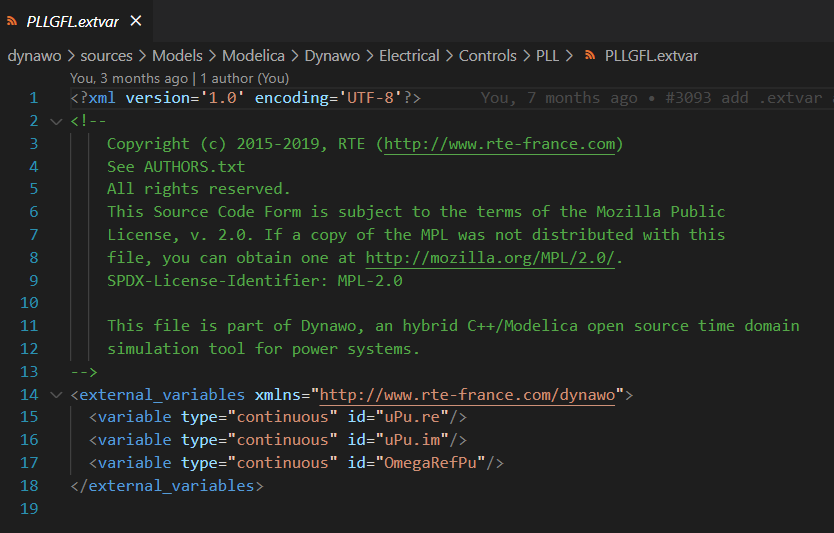
\includegraphics[scale = 0.5]{Figure_1VSC/PLLGFL_extvar_Dynawo.PNG}
    \caption{Example of external variables file (PLL model)}
    \label{fig:PLLGFL_extvar_Dynawo}
    \end{figure}

\end{enumerate}

After the implementation of the model in Dynawo Modelica library and the creation of the necessary "INIT" and "extvar" files, the model can be now used in Dynawo as part of 1-VSC system. For this purpose 4 XML files are needed: ".job", ".iidm", ".dyn", ".par". For more details about the purpose and content of each file we refer to the official Dynawo documentation. Examples of how to use these files to run system simulations can be found in the official Dynawo repository.

\subsection{EMTP implementation}
The previously described test model is not available in EMTP libraries, and therefore it was made from scratch. Currently the commercial version of EMTP is controlled by EDF, Hydro-Québec and RTE. It is designed to model, simulate, and analyze electrical power systems and their components. EMTP allows for detailed and accurate modeling of electrical components, including transmission lines, transformers, generators, loads, and it is capable to simulate various types of transients, including both time-domain and frequency-domain analysis. Offering a graphical user interface makes it very user-friendly, and the components can be modeled as blocks and easily connected together. In the developed model, two parts can be distinguished, the grid following control and the injector (grid interface). \figurename~\ref{fig:1-VSC-model} shows the implemented 1-VSC system, and \figurename~\ref{fig:GFL_model_EMTP} the GFL model.
\begin{figure}[H]
    \centering
    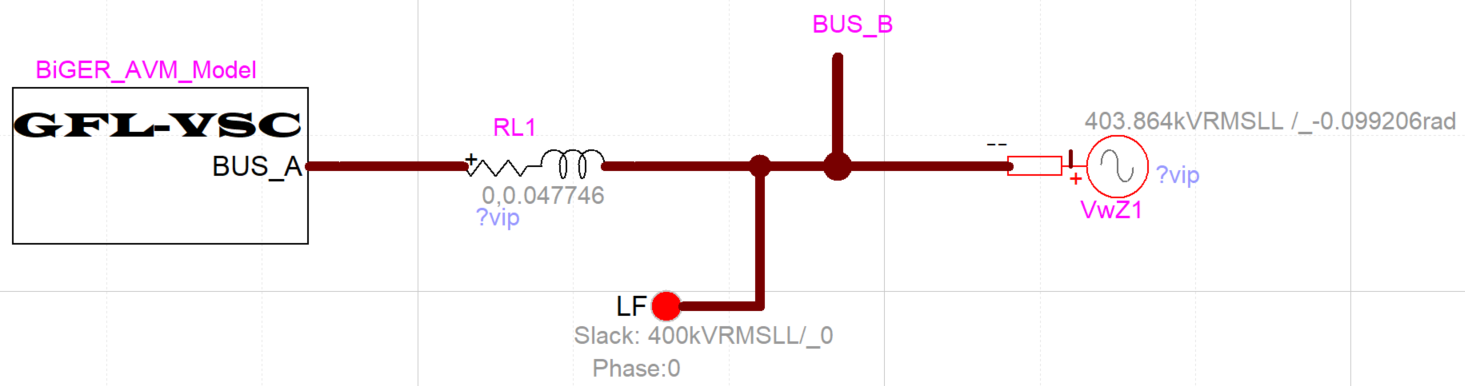
\includegraphics[scale = 0.4]{Figure_1VSC/1VSC_EMTP.png}
    \caption{1-VSC test system in EMTP showing the GFL and the infinite bus.}
    \label{fig:1-VSC-model}
\end{figure}
The obtained values from the 1VSC\_Control are used as input signals into the cV1, cV4 and cV5 blocks, which represent voltage sources. They are used to generate a three-phase voltage signal, which is injected into the grid. The blocks AC8, AC9 and AC10 are used to set the initial conditions of the voltage.
\begin{figure}[H]
    \centering
    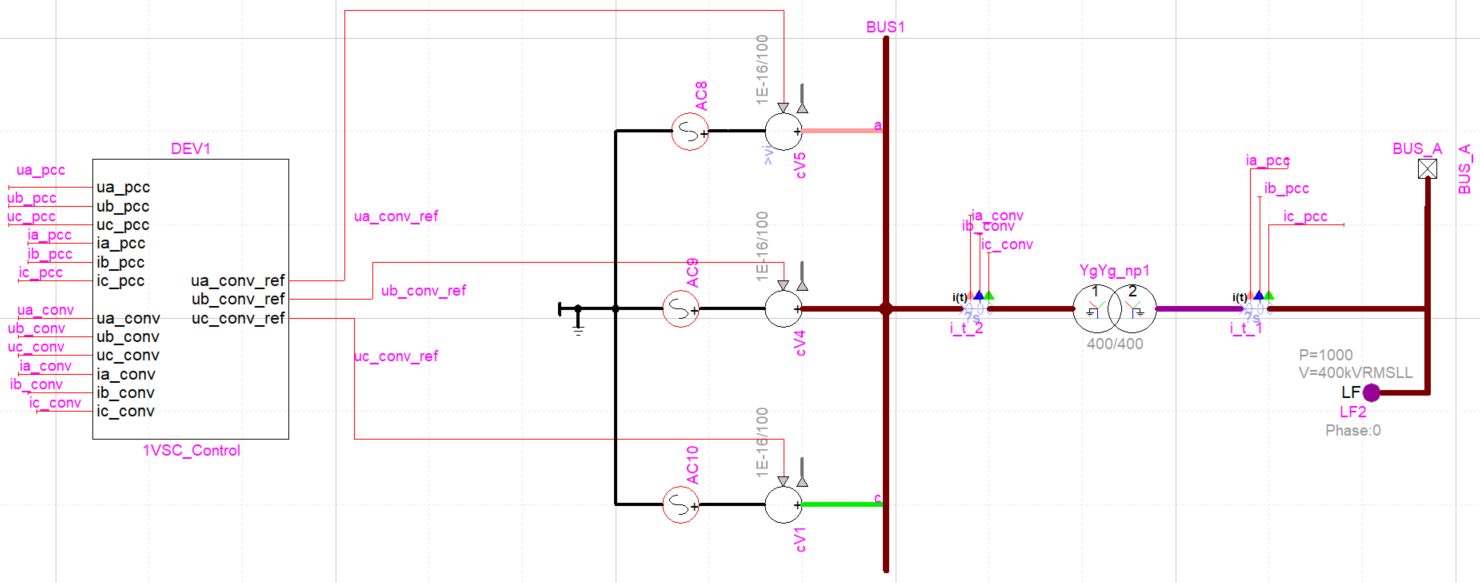
\includegraphics[scale = 0.4]{Figure_1VSC/GFL_EMTP.png}
    \caption{GFL model - EMTP}
    \label{fig:GFL_model_EMTP}
\end{figure}

First, the measurements need to be taken, and transformed into the DQ0 domain, presented in \figurename~\ref{fig:1-VSC-model_measurements}, which are used to calculate the active and reactive power.

Initialization:\\
\textbf{Set of Input Parameters}
\begin{table}[H]
\centering
\begin{tabular}{|l | l |l |}  
\hline
Parameter & Value & Definition \\
 \hline
 \hline
   $F$ &  $50$ & System frequency (in Hz) \\
  \hline
   $S_{nom}$ &  $1200*10^6$ & Nominal apparent power of synchronous machine (SM) (in MVA) \\
  \hline
  $U_{pcc}$ &  $400*10^3$ & Base value of PCC L-L RMS Voltage (in volt) \\
  \hline
$U_{conv}$ &  $400*10^3$ & Base value of SM L-L RMS Voltage (in volt) \\
\hline
 $P_{ref}$ &  $1000*10^6$ & Nominal active power of SM turbine (in MW) \\
  \hline
   $R_t$ &  $0.0005$ & Step-up transformer resistance (in p.u.) \\
  \hline
  $L_t$ &  $0.15$ & Step-up transformer reactance (in p.u.) \\
  \hline
  $Tr_{ratio}$ &  $1.02$ & Step-up transformer ratio  \\
  \hline
  $U_{pcc_{ref}}$ &  $1.00$ & Initial voltage magnitude of bus 4031 (in p.u.)  \\
  \hline
  $U_{conv_{pu}}$ &  $0.99878$ & Initial voltage magnitude of SM bus G12 (in p.u.)  \\
  \hline
  $\omega_{ref_{pu}}$ &  $1$ & reference angular speed (in p.u.)  \\
  \hline
\end{tabular}
\end{table}
\textbf{Load Flow result:}\\ 
1) $V_g$= Initial PCC phase voltage  ( rms) in p.u.\\
2) $P_0$= Initial active power (p.u)\\
3) $Q_0$= Initial reactive power (p.u)\\
4) $\theta_g$= Initial angle of PLL loop in rad.\\

\textbf{Initial value calculation:}\\
$v_{d0} = V_g$\\
$vq0 = 0$//
$v_{gd} = Vg*cos(theta_g)$\\
$v_{gq} = Vg*sin(theta_g)$\\
$ig_{real} = P_0 / (V_g/Tr_{ratio})$\\
$ig_{imag} = -Q_0 / (V_g/Tr_{ratio})$\\
$Vm_{real} = V_g/Tr_{ratio} + ig_{real}*R_t - ig_{imag} * L_t$\\
$Vm_{imag} = + ig_{imag}* R_t  + ig_{real}*L_t$\\
$Vm = \sqrt{Vm_{real}^2 + Vm_{imag}^2}$\\
$Vm_{amp} = Vm * U_{conv}*\sqrt{2/3}$\\
$\theta_m=atan(Vm_{imag}/Vm_{real}) + \theta_g$\\
$\phi_1 = \theta_m*180/PI$\\
$\phi_2 = \phi_1 - 120$\\
$\phi_3 = \phi_1 + 120$\\

\textbf{measured signal}\\ 
$u_{{a,b,c}_{pcc}}$ is the instantaneous PCC voltage for all 3 phases\\
$i_{{a,b,c}_{pcc}}$ is the instantaneous PCC current for all 3 phases\\
All measured signals entering the
control systems are, first, converted to per unit on the respective base. 
$U_{pcc-base}$= $U_{pcc}$\\
$I_{pcc-base}$= $S_{nom}/ U_{pcc}$


\textbf{Calculated signal}\\ 
$u_d, u_q$ - d,q component of $u_{{a,b,c}_{pcc}}$\\
$i_{d_{pcc}}, i_{q_{pcc}}$ - d,q component converter side current $i_{{a,b,c}_{pcc}}$ \\
$i_d,i_q$ - d, q component of current on the converter side obtained by multiplying $i_{d_{pcc}}, i_{q_{pcc}}$ with $Tr_{ratio}$\\
$p_{pcc}$=$u_d*i_{d_{pcc}} + u_q*i_{q_{pcc}}$\\
$q_{pcc}$=$u_q*i_{d_{pcc}} - u_d*i_{q_{pcc}}$\\
$u_{sec}=\sqrt{(\frac{u_d}{Tr_{ratio}})^2 + (\frac{u_q}{Tr_{ratio}})^2}$\\
$U_{conv}^0=\sqrt{(u_{sec} + i_d*R_t - i_q*L_t)^2 + (i_q*R_t +i_d*L_t)^2}$\\

The grid-following converter control for the phase-locked loop (PLL), d-q current control, active power control, and voltage/reactive power control loop is the same as described in the 1VSC control or the HVDC1 control of the 4VSC system. In EMTP, as previously mentioned, average value models (AVMs) are employed, which approximate system dynamics by neglecting switching details. 
This approach simplifies the circuit by not explicitly representing IGBTs and their diodes, thus excluding lower-level control. Consequently, it requires significantly fewer computational resources and allows for larger integration time steps, resulting in much faster computations. Vector Current Control is implemented to regulate the instantaneous active and reactive powers independently through a fast inner current control loop. The VSC behavior is modeled using controlled voltage on the AC side, while the DC side is not modeled, as the focus is entirely on AC grid dynamics. The VSC connects to the grid through a transformer, with its resistance and reactance acting as a filter, eliminating the need for an additional LC filter. Transformer magnetization parameters are neglected. Also, no protection scheme is modeled to disconnect the VSCs from the system at the time of start up, disturbances like DC overcurrent or deep voltage sag detectors to protect the converter. Only an additional initialization scheme is introduced to improve the initial transient during the Start up.  Table \ref{tab:HistoryVSC} details the initialization of the different controller blocks in EMTP.
 \begin{table}[H]
\centering
\caption{History Block}
\begin{tabular}{|c|c|}
    \hline
For Integrator PLL: & ${\Tilde{\omega}}$ (0)= 0 \\
\hline
For APC $\frac{1}{(1+s.T_{LPF})}$ block: & $P_0$\\
\hline
For Integrator APC: &$ig_{real}$ \\
\hline
For V/QPC $\frac{1}{(1+s.T_{LPF})}$ block: & $U_{conv}^0$\\
\hline
For Integrator V/QPC: &$ig_{imag}$ \\
\hline
For Integrator Current Control $\upsilon_{md}$: &$(Vm_{real}- \frac{u_d}{Tr_ratio} + \Tilde{\omega}*L_t*i_q)$ \\
\hline
For Integrator Current Control $\upsilon_{mq}$: &$(Vm_{imag}- \Tilde{\omega}*L_t*i_d)$ \\
    \hline
\end{tabular}
\label{HistoryVSC}
\end{table}

\begin{figure}[H]
    \centering
    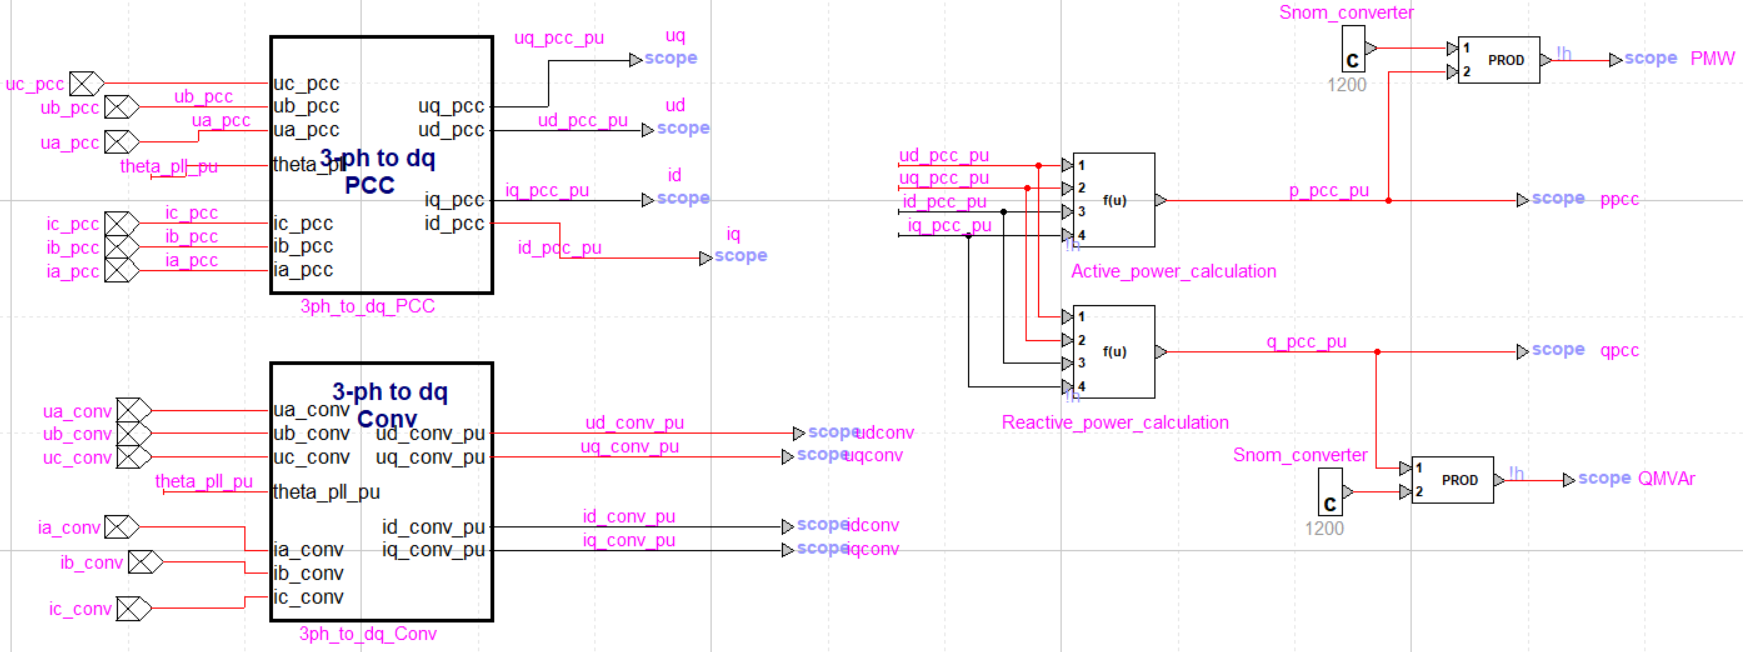
\includegraphics[scale = 0.35]{Figure_1VSC/1VSC_model_measurements.png}
    \caption{GFL model, measurements, EMTP}
    \label{fig:1-VSC-model_measurements}
\end{figure}
The blocks \textit{3-ph to dq} are used to transfer the values into the DQ0 system using the equation \eqref{dq0_equation}. 
The active and reactive power are calculated as:
\begin{equation}
    P = u_{d,pcc}i_{d,pcc} + u_{q,pcc}i_{q,pcc}
\end{equation}
\begin{equation}
    Q = u_{q,pcc}i_{d,pcc} - u_{d,pcc}i_{q,pcc}
\end{equation}
It is important to mention that the all values are translated into the per unit system before the calculations are done. The grid following control shown in \figurename~\ref{fig:1VSC_control_EMTP} consists of:
\begin{itemize}
    \item PLL
    \item Inner current loop
    \item Active power loop
    \item Reactive power loop
\end{itemize}
In \figurename~\ref{fig:1VSC_control_EMTP}, the block $f(u)$ is used to convert the values into the per unit system:
\begin{equation}
f(u) = \frac{u}{V_{base}},    
\end{equation}
and the "c" blocks are constants for the referent value of the active power and the referent value of the converter voltage.

\begin{figure}[H]
    \centering
    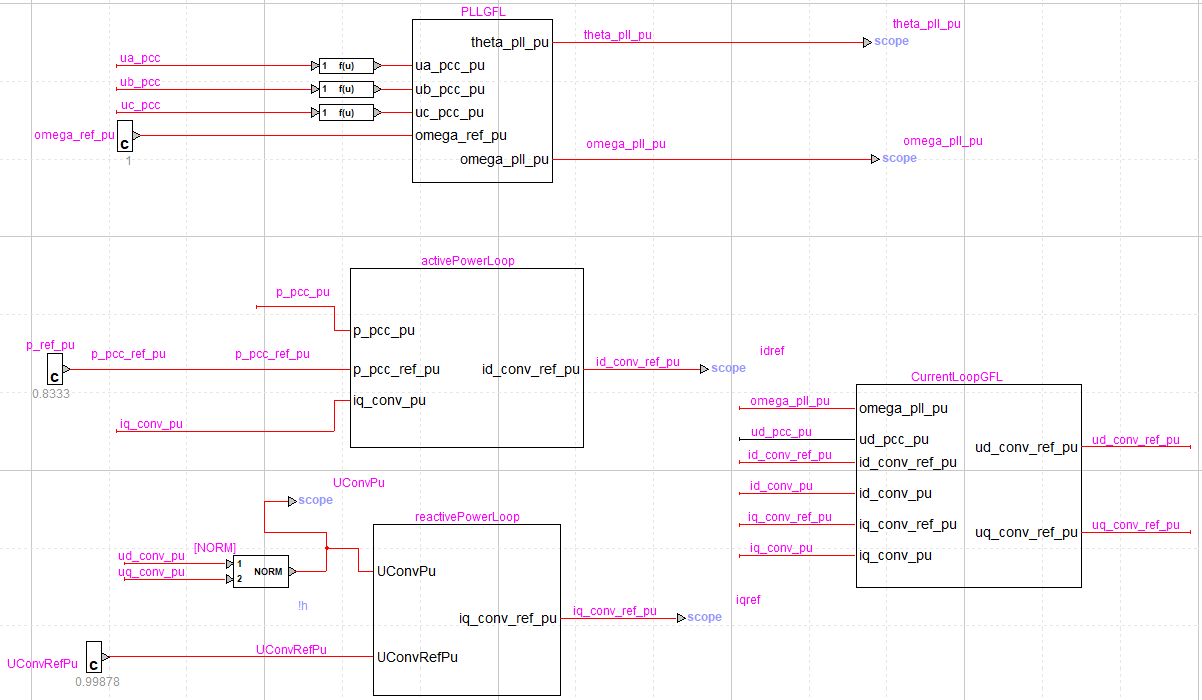
\includegraphics[scale = 0.51]{Figure_1VSC/1VSC_control_EMTP.png}
    \caption{Grid following control structure - EMTP}
    \label{fig:1VSC_control_EMTP}
\end{figure}
The PLL is modeled as in the following figure:
\begin{figure}[H]
    \centering
    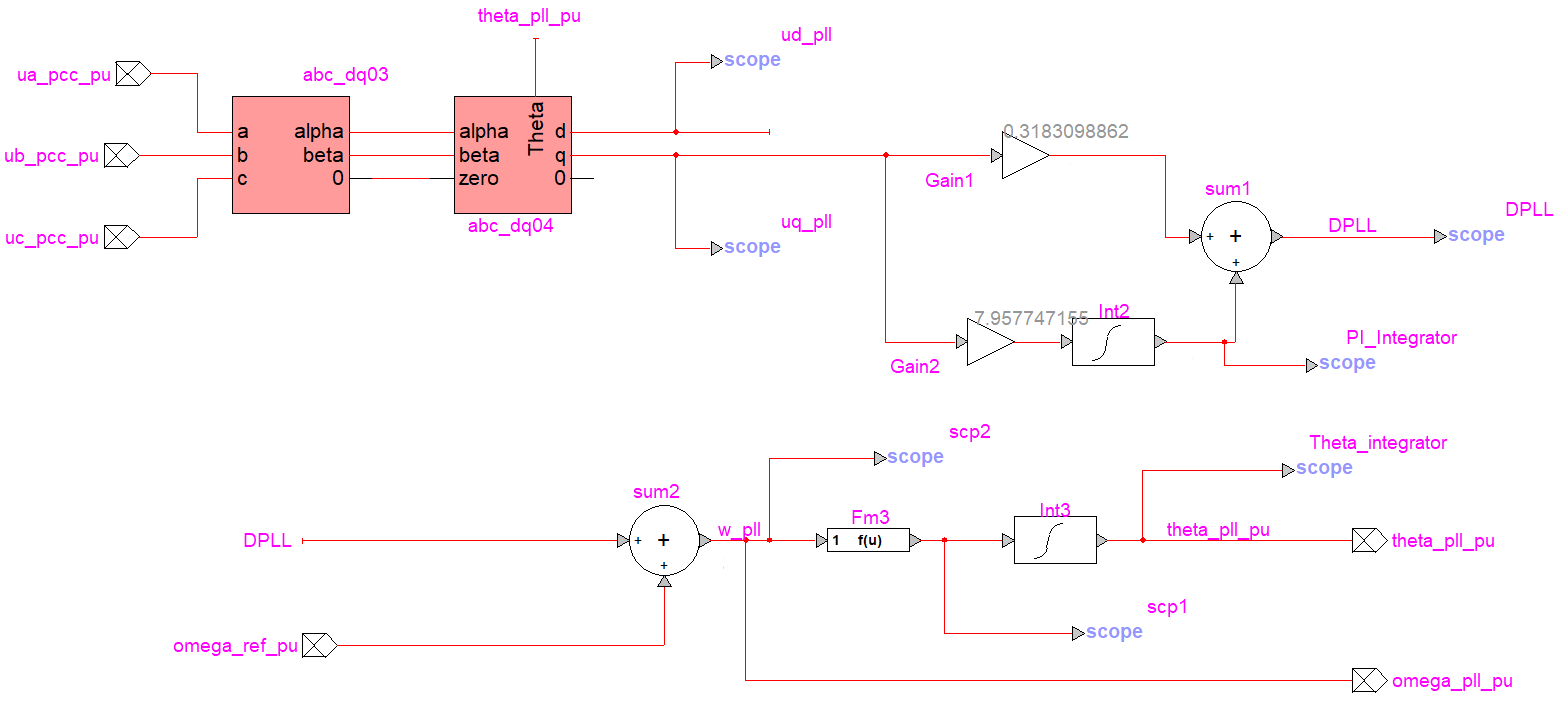
\includegraphics[scale = 0.5]{Figure_1VSC/1VSC_PLL_EMTP.png}
    \caption{PLL structure - EMTP}
    \label{fig:1VSC_PLL_EMTP}
\end{figure}
The Fm8 block is a function block, and the implemented function is:
\begin{equation}
    f(u) = u\cdot 2\pi50
\end{equation}
The current control which is implemented in EMTP using build-in blocks is shown in the next figure.
\begin{figure}[H]
    \centering
    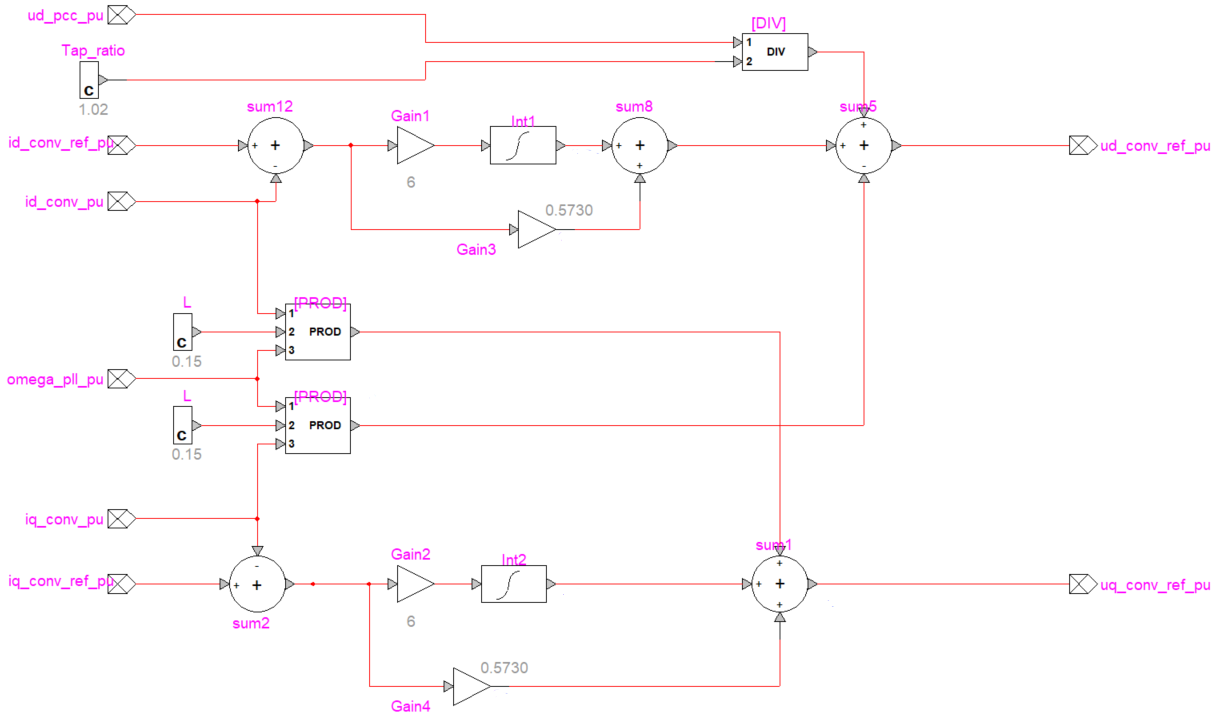
\includegraphics[scale = 0.63]{Figure_1VSC/1VSC_current_control_EMTP.png}
    \caption{Current control structure - EMTP}
    \label{fig:1VSC_current_control_EMTP}
\end{figure}
\figurename~\ref{fig:1VSC_active_power_EMTP} shows the active current loop, and the structure of the active current limiter is presented in \figurename~\ref{fig:1VSC_active_current_limiter_EMTP}.
\begin{figure}[H]
    \centering
    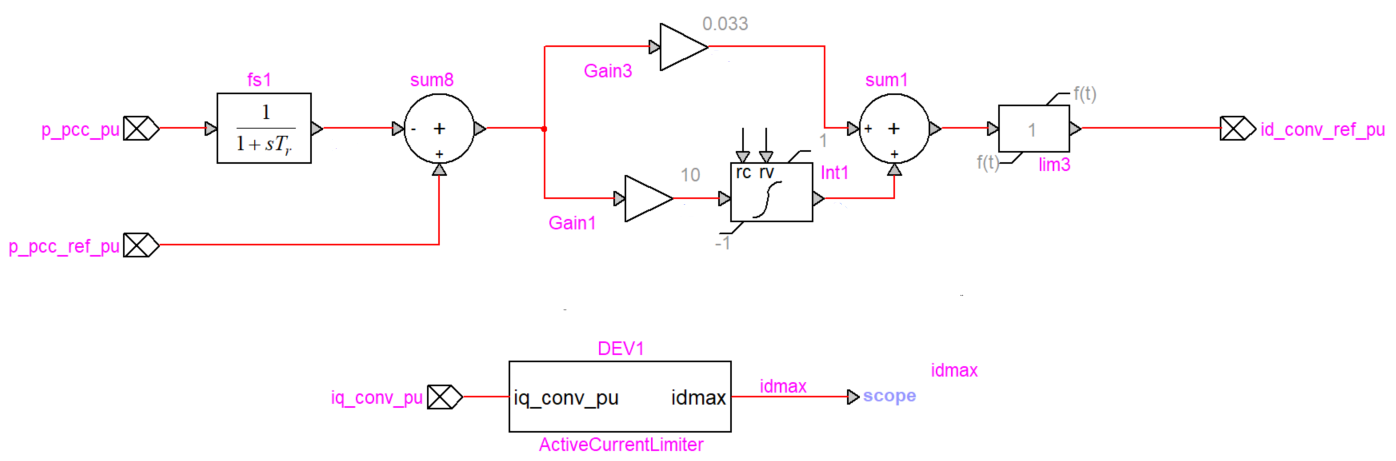
\includegraphics[scale = 0.55]{Figure_1VSC/1VSC_active_power_EMTP.png}
    \caption{Active power loop - EMTP}
    \label{fig:1VSC_active_power_EMTP}
\end{figure}
In \figurename~\ref{fig:1VSC_active_power_EMTP} rc represents reset control, and rv the reset value. Output is reset to reset value (rv) when reset control (rc) is $>$ 0. Also, $f(t)$ represents the limits which are given as functions. The gain in \figurename~\ref{fig:1VSC_active_current_limiter_EMTP} has the value $1/T$ which is equal to 500.

\begin{figure}[H]
    \centering
    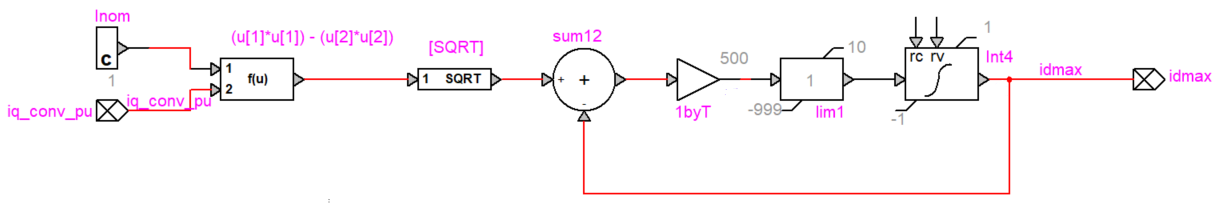
\includegraphics[scale = 0.62]{Figure_1VSC/1VSC_active_current_limiter_EMTP.png}
    \caption{Active current limiter - EMTP}
    \label{fig:1VSC_active_current_limiter_EMTP}
\end{figure}
The reactive power loop is shown in \figurename~\ref{fig:1VSC_reactive_power_EMTP}, and the voltage control is used.
\begin{figure}[H]
    \centering
    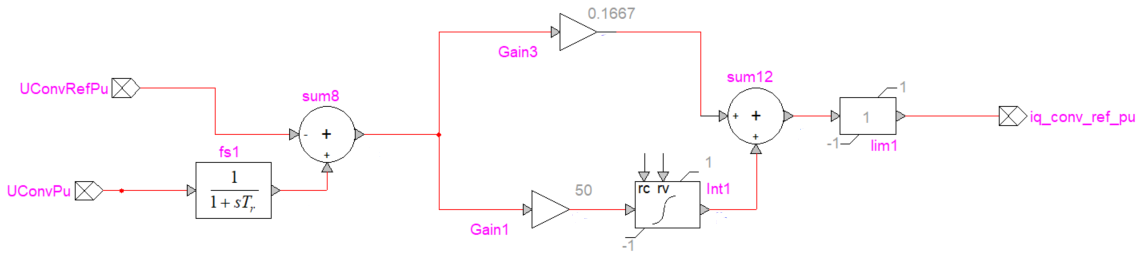
\includegraphics[scale = 0.67]{Figure_1VSC/1VSC_reactive_power_EMTP.png}
    \caption{Reactive power loop - EMTP}
    \label{fig:1VSC_reactive_power_EMTP}
\end{figure}
The second part is the injector, where the inverse DQ0 transformation is performed, and the obtained voltages are injected into the grid, as shown in \figurename~\ref{fig:1VSC_injector_EMTP}.
\begin{figure}[H]
    \centering
    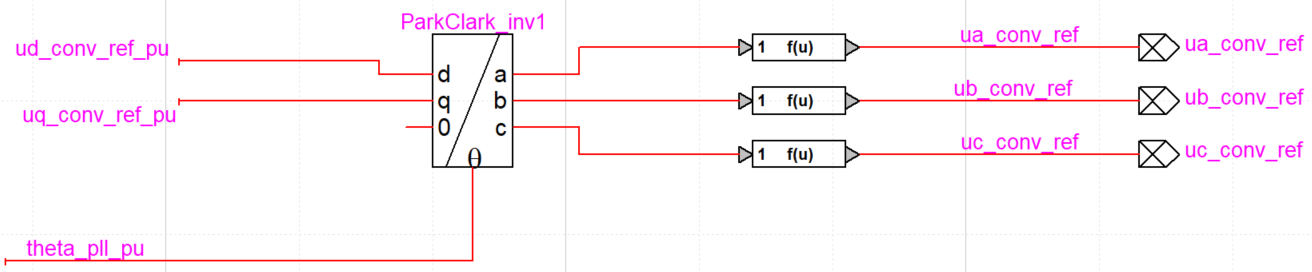
\includegraphics[scale = 0.47]{Figure_1VSC/1VSC_injector_EMTP.png}
    \caption{Injector - EMTP}
    \label{fig:1VSC_injector_EMTP}
\end{figure}
The blocks $f(u)$ are function blocks, which are used to convert back from the per unit system:
\begin{equation}
    f(u) = u\sqrt{\frac{2}{3}}V_{base}
\end{equation}

\subsection{Simulation results}
After the implementation of the test model and test system in the different simulators, multiple dynamic simulations are run, and the results are compared to each other. The simulations settings of the different simulators are summarized in the following table:

\begin{table}[H]
\centering
\caption{1-VSC simulation settings}
\begin{tabular}{lcccc}
\hline
                   & \textbf{STEPSS}                  & \textbf{OpenModelica} & \textbf{Dynawo} & \textbf{EMTP} \\ \hline
Domain             & RMS                              & RMS                   & RMS             & EMT           \\ \hline
Duration           & 8s                               & 8s                    & 8s              & 8s            \\ \hline
Step size          & 1ms (fix)                        & 1ms (fix)             & 1ms (fix)       & 50us (fix)    \\ \hline
Solver             & DAE                              & DAE                   & DAE             & Nodal         \\ \hline
Integration method & BDF & Dassl                 & BE  & Trapezoidal   \\ \hline
\end{tabular}
\label{1VSC_simulation_params}
\end{table}


To following events and scenarios are used to compare the results obtained from STEPSS, OpenModelica, Dynawo and EMTP:
\begin{itemize}
    \item[1.] Event - Setpoint change
    \begin{itemize}
        \item[1.] Scenario - Reduce active power setpoint  by -0.05 p.u. (converter base power)
        \item[2.] Scenario - Increase active power setpoint by 0.5 p.u. (converter base power)
        \item[3.] Scenario - Increase voltage setpoint by 0.02 p.u. (network base voltage)
        \item[4.] Scenario - Increase voltage setpoint by 0.2 p.u. (network base voltage) 
    \end{itemize}
    \item[2.] Event - Fault
    \begin{itemize}
        \item[5.] Scenario - Fault at converter PCC
        \item[6.] Scenario - Fault at infinite bus 
    \end{itemize}
\end{itemize}

The converter model parameters which are used in the 1-VSC test system are summarized in Table \ref{table_1VSC_model_parameters}.
\begin{table}[H]
\centering
\caption{1-VSC converter dynamic parameters}
\begin{tabular}{ll|l}
\multicolumn{2}{l|}{}                                                  & 1-VSC    \\ \hline
\multicolumn{2}{l|}{Snom (MVA)}                                              & 1200     \\ \hline
\multicolumn{2}{l|}{P (MW)}                                            & 1000     \\ \hline
\multicolumn{2}{l|}{Q (MVAr)}                                          & 47       \\ \hline
\multicolumn{2}{l|}{Vpcc (p.u.)}                                              & 1        \\ \hline
\multicolumn{2}{l|}{Angle - pcc (rad)}                                 & 0.093887 \\ \hline
\multicolumn{2}{l|}{Vconv (p.u.)}                                      & 0.99878  \\ \hline
\multicolumn{2}{l|}{R (p.u.)}                                                 & 0.005    \\ \hline
\multicolumn{2}{l|}{L (p.u.)}                                                 & 0.15     \\ \hline
\multicolumn{1}{l|}{\multirow{2}{*}{Current loop}}        & Kp (p.u.)        & 0.5730   \\ \cline{2-3} 
\multicolumn{1}{l|}{}                                     & Ki (pu/s)         & 6        \\ \hline
\multicolumn{1}{l|}{\multirow{6}{*}{Active power loop}}   & Tlpf (s)       & 0.0033   \\ \cline{2-3} 
\multicolumn{1}{l|}{}                                     & Kpp (pu)       & 0.0333   \\ \cline{2-3} 
\multicolumn{1}{l|}{}                                     & Kip (pu/s)       & 10       \\ \cline{2-3} 
\multicolumn{1}{l|}{}                                     & Trlim (s)     & 0.002    \\ \cline{2-3} 
\multicolumn{1}{l|}{}                                     & dP/dt\_min (pu/s) & -999     \\ \cline{2-3} 
\multicolumn{1}{l|}{}                                     & dP/dt\_max (pu/s)& 10       \\ \hline
\multicolumn{1}{l|}{\multirow{3}{*}{Reactive power loop}} & Kpv (pu)       & 0.1670   \\ \cline{2-3} 
\multicolumn{1}{l|}{}                                     & Kiv (pu/s)       & 50       \\\cline{2-3} 
\multicolumn{1}{l|}{}                                     & tau        & 0.1      \\ \hline
\multicolumn{1}{l|}{\multirow{2}{*}{PLL}}                 & Vpllb  (p.u.)    & 0.4      \\ \cline{2-3} 
\multicolumn{1}{l|}{}                                     & Vpllu  (p.u.)    & 0.5      \\ \hline
\multicolumn{2}{l|}{Imax (p.u.)}                                              & 1        \\ \hline
\multicolumn{2}{l|}{Vs1 (p.u.)}                                               & 0.95     \\ \hline
\multicolumn{2}{l|}{Vs2 (p.u.)}                                               & 0.5      \\ \hline
\multicolumn{2}{l|}{iqmax (p.u.)}                                             & 99      
\end{tabular}
\label{table_1VSC_model_parameters}
\end{table}

To compare the results, the obtained sine waves from the EMTP simulation are translated into RMS signals. In EMTP we are measuring the peak phase to ground value. To get the amplitude of the three-phase signals we use the following formula:
\begin{equation}
    V_{amp} = \sqrt{\frac{2}{3}}\sqrt{v_a(t)^2 + v_b(t)^2 + v_c(t)^2}
    \label{sine_to_RMS}
\end{equation}
$V_{amp}$ represents the phase to ground amplitude, and to get the RMS line to line value we need to multiply $V_{amp}$ by $\sqrt{\frac{3}{2}}$.
The simulation results are presented in the following figures, where the used software are compared.
\begin{figure}[H]
    \centering
    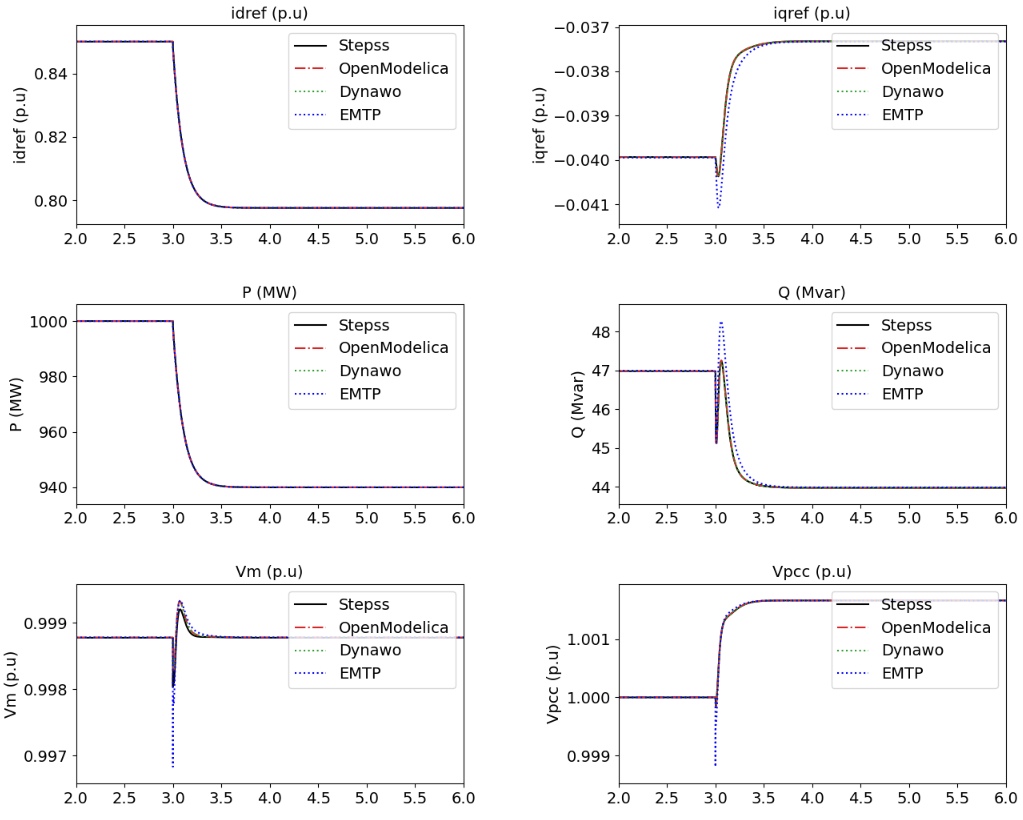
\includegraphics[scale = 0.61]{Simulation_results/Event1Scenario1.png}
    \caption{Event 1, Scenario 1 - Reduce active power setpoint  by -0.05 p.u. (converter base power)}
    \label{fig:Event1Scenario1}
\end{figure}
\begin{figure}[H]
    \centering
    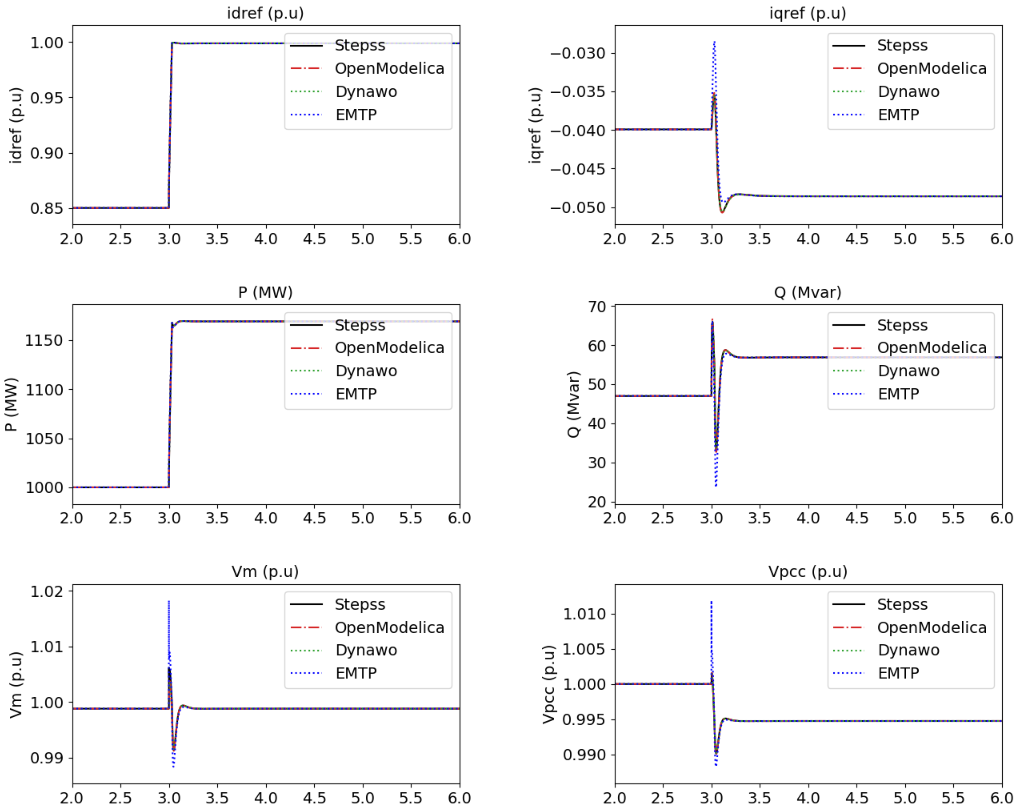
\includegraphics[scale = 0.61]{Simulation_results/Event1Scenario2.png}
    \caption{Event 1, Scenario 2 - Increase active power setpoint by 0.5 p.u. (converter base power)}
    \label{fig:Event1Scenario2}
\end{figure}
\begin{figure}[H]
    \centering
    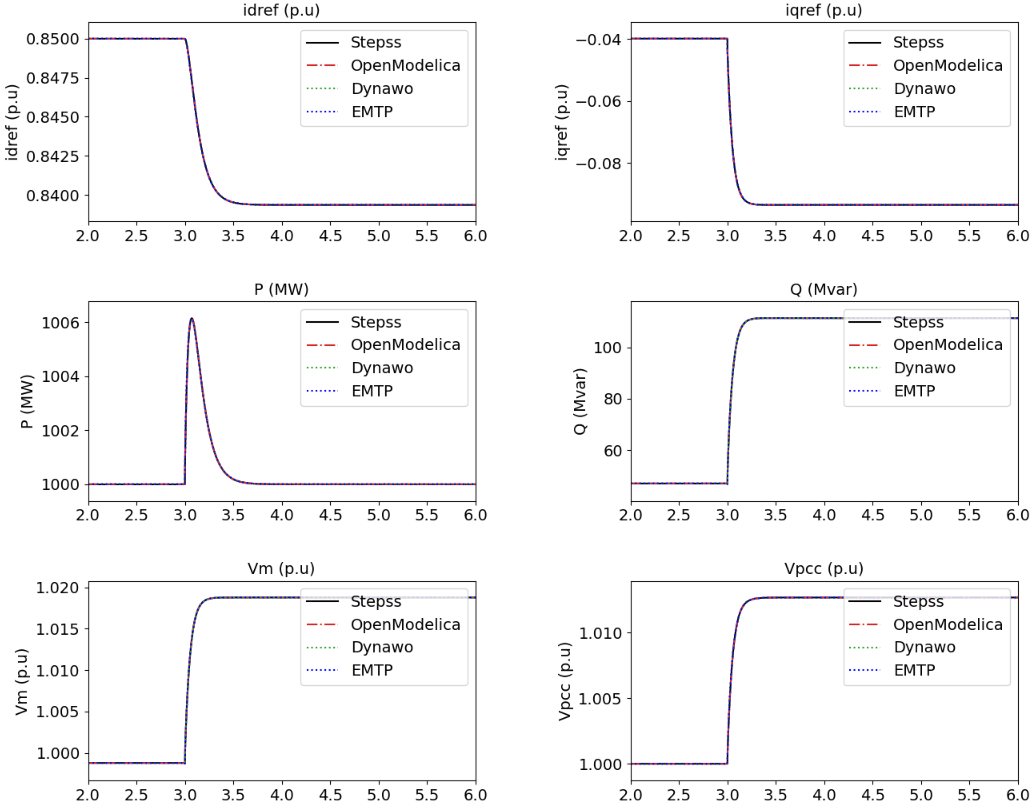
\includegraphics[scale = 0.61]{Simulation_results/Event1Scenario3.png}
    \caption{Event 1, Scenario 3 - Increase voltage setpoint by 0.02 p.u. (network base voltage)}
    \label{fig:Event1Scenario3}
\end{figure}
\begin{figure}[H]
    \centering
    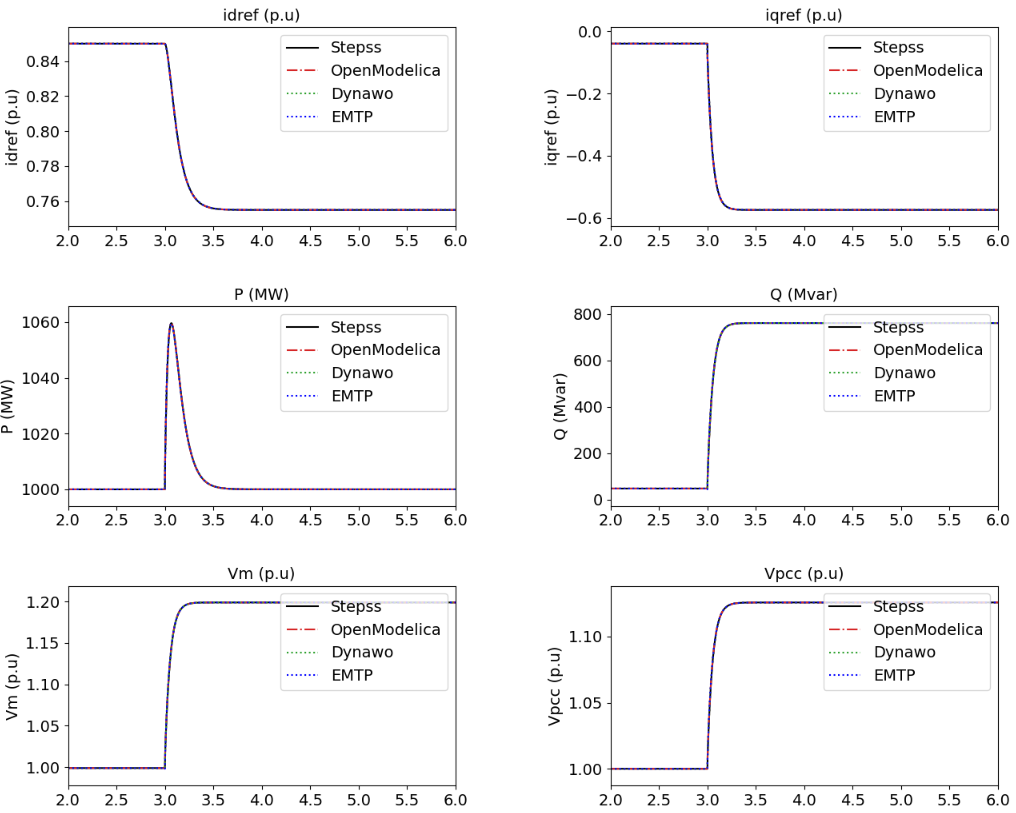
\includegraphics[scale = 0.61]{Simulation_results/Event1Scenario4.png}
    \caption{Event 1, Scenario 4 - Increase voltage setpoint by 0.2 p.u. (network base voltage)}
    \label{fig:Event1Scenario4}
\end{figure}
\begin{figure}[H]
    \centering
    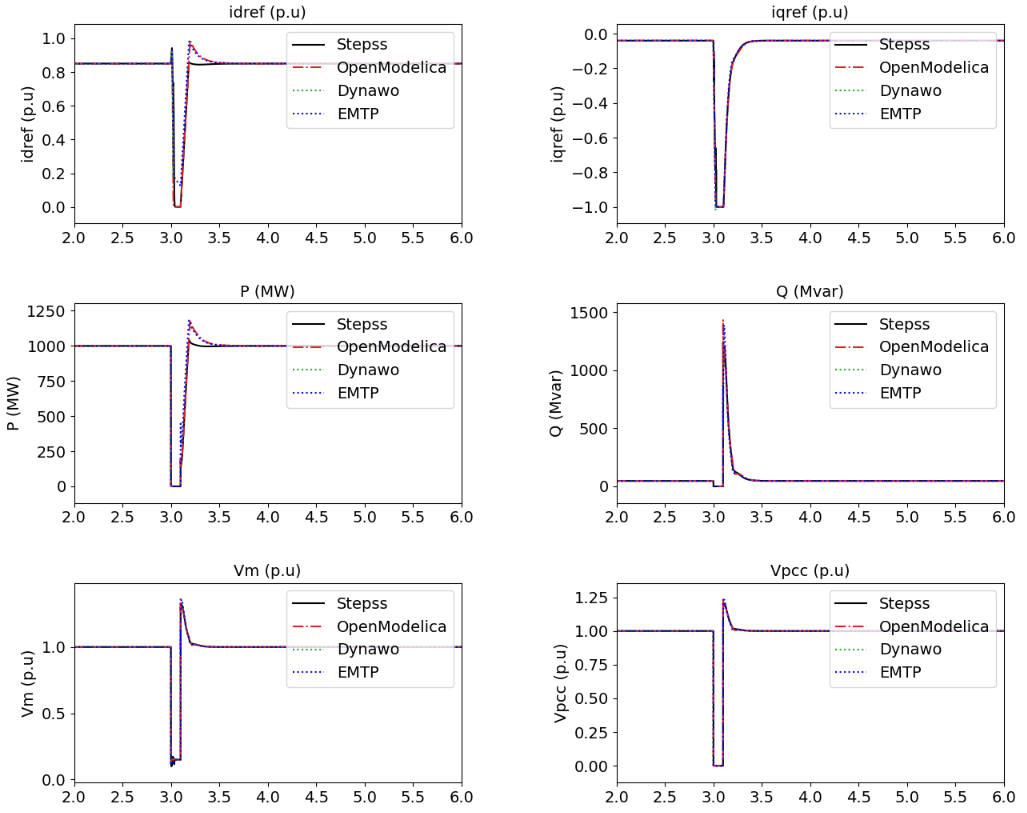
\includegraphics[scale = 0.61]{Simulation_results/Event2Scenario5.png}
    \caption{Event 2, Scenario 5 - Fault at converter PCC}
    \label{fig:Event2Scenario5}
\end{figure}
\begin{figure}[H]
    \centering
    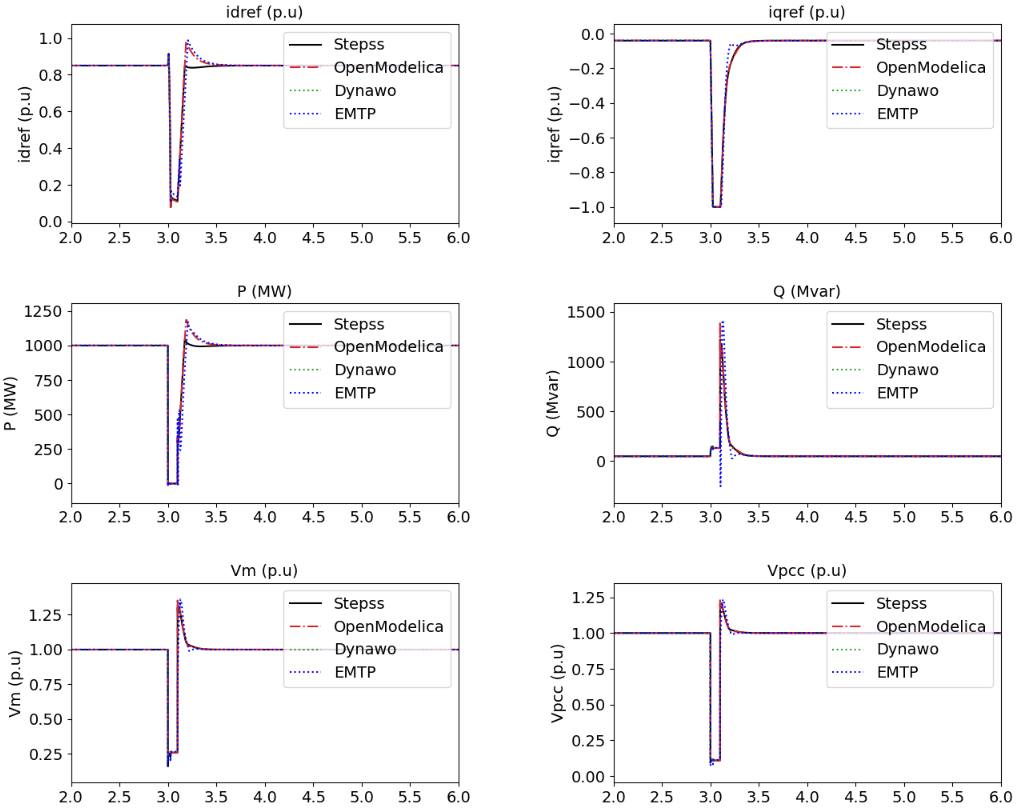
\includegraphics[scale = 0.61]{Simulation_results/Event2Scenario6.png}
    \caption{Event 2, Scenario 6 - Fault at infinite bus }
    \label{fig:Event2Scenario6}
\end{figure}
The steady-state values of the observed signals after the transient are displayed in Table \ref{1VSC_results_table}.
\begin{table}[H]
\centering
\caption{Steady-state values after the transient}
\begin{tabular}{ll|l|l|l|l|l|l}
                                                   &              & \multicolumn{1}{c|}{\begin{tabular}[c]{@{}c@{}}Event 1\\ Scenario 1\end{tabular}} & \multicolumn{1}{c|}{\begin{tabular}[c]{@{}c@{}}Event 1\\ Scenario 2\end{tabular}} & \multicolumn{1}{c|}{\begin{tabular}[c]{@{}c@{}}Event 1\\ Scenario 3\end{tabular}} & \multicolumn{1}{c|}{\begin{tabular}[c]{@{}c@{}}Event 1\\ Scenario 4\end{tabular}} & \multicolumn{1}{c|}{\begin{tabular}[c]{@{}c@{}}Event 2\\ Scenario 5\end{tabular}} & \multicolumn{1}{c}{\begin{tabular}[c]{@{}c@{}}Event 2\\ Scenario 6\end{tabular}} \\ \hline
                                                   
\multicolumn{1}{l|}{\parbox[t]{2mm}{\multirow{4}{*}{\rotatebox[origin=c]{90}{idref (p.u.)}}}} & STEPSS       & 0.7976691                                                                         & 0.9988185                                                                         & 0.8393613                                                                         & 0.754999                                                                          & 0.8499943                                                                         & 0.8499942                                                                        \\
\multicolumn{1}{l|}{}                              & OpenModelica & 0.7976723                                                                         & 0.9988185                                                                         & 0.8393641                                                                         & 0.755002                                                                          & 0.8499977                                                                         & 0.849997                                                                         \\
\multicolumn{1}{l|}{}                              & Dynawo       & 0.797673                                                                          & 0.998819                                                                          & 0.839650                                                                          & 0.755003                                                                          &                                                                                   &                                                                                  \\
\multicolumn{1}{l|}{}                              & EMTP         & 0.797674                                                                          & 0.998817                                                                          & 0.839366                                                                          & 0.755003                                                                          & 0.8499998                                                                         & 0.849650                                                                         \\ \hline
\multicolumn{1}{l|}{\parbox[t]{2mm}{\multirow{4}{*}{\rotatebox[origin=c]{90}{iqref (p.u.)}}}} & STEPSS       & -0.037318                                                                         & -0.048595                                                                         & -0.093446                                                                         & -0.57442                                                                          & -0.039929                                                                         & -0.039928                                                                        \\
\multicolumn{1}{l|}{}                              & OpenModelica & -0.037318                                                                         & -0.048596                                                                         & -0.093446                                                                         & -0.57442                                                                          & -0.039933                                                                         & -0.039933                                                                        \\
\multicolumn{1}{l|}{}                              & Dynawo       & -0.037318                                                                         & -0.048594                                                                         & -0.093445                                                                         & -0.57442                                                                          &                                                                                   &                                                                                  \\
\multicolumn{1}{l|}{}                              & EMTP         & -0.037329                                                                         & -0.048607                                                                         & -0.093455                                                                         & -0.57442                                                                          & -0.039943                                                                         & -0.039925                                                                        \\ \hline
\multicolumn{1}{l|}{\parbox[t]{2mm}{\multirow{4}{*}{\rotatebox[origin=c]{90}{P (MW)}}}}       & STEPSS       & 939.9936                                                                          & 1168.893                                                                          & 999.9936                                                                          & 999.9936                                                                          & 999.9936                                                                          & 999.9936                                                                         \\
\multicolumn{1}{l|}{}                              & OpenModelica & 939.9996                                                                          & 1168.896                                                                          & 999.9999                                                                          & 999.9996                                                                          & 999.9996                                                                          & 999.9996                                                                         \\
\multicolumn{1}{l|}{}                              & Dynawo       & 940.0008                                                                          & 1168.896                                                                          & 1000.0008                                                                         & 1000.0008                                                                         &                                                                                   &                                                                                  \\
\multicolumn{1}{l|}{}                              & EMTP         & 939.99972                                                                         & 1168.8927                                                                         & 999.99983                                                                         & 999.9998                                                                          & 999.9998                                                                          & 999.9995                                                                         \\ \hline
\multicolumn{1}{l|}{\parbox[t]{2mm}{\multirow{4}{*}{\rotatebox[origin=c]{90}{Q (MVAr)}}}}     & STEPSS       & 43.9765                                                                           & 56.87024                                                                          & 111.3297                                                                          & 760.8226                                                                          & 46.9756                                                                           & 46.97502                                                                         \\
\multicolumn{1}{l|}{}                              & OpenModelica & 43.9775                                                                           & 56.87088                                                                          & 111.3295                                                                          & 760.8245                                                                          & 46.9802                                                                           & 46.98031                                                                         \\
\multicolumn{1}{l|}{}                              & Dynawo       & 43.9764                                                                           & 56.8692                                                                           & 111.3288                                                                          & 760.8228                                                                          &                                                                                   &                                                                                  \\
\multicolumn{1}{l|}{}                              & EMTP         & 43.9900                                                                           & 56.8837                                                                           & 111.3409                                                                          & 760.8226                                                                          & 46.9928                                                                           & 46.97203                                                                         \\ \hline
\multicolumn{1}{l|}{\parbox[t]{2mm}{\multirow{4}{*}{\rotatebox[origin=c]{90}{Vm (p.u.)}}}}    & STEPSS       & 0.998777                                                                          & 0.998777                                                                          & 1.018778                                                                          & 1.19877                                                                           & 0.99877                                                                           & 0.99877                                                                          \\
\multicolumn{1}{l|}{}                              & OpenModelica & 0.998780                                                                          & 0.998780                                                                          & 1.018780                                                                          & 1.19878                                                                           & 0.99878                                                                           & 0.99878                                                                          \\
\multicolumn{1}{l|}{}                              & Dynawo       & 0.998780                                                                          & 0.998780                                                                          & 1.018780                                                                          & 1.19878                                                                           &                                                                                   &                                                                                  \\
\multicolumn{1}{l|}{}                              & EMTP         & 0.99878                                                                           & 0.99878                                                                           & 1.018780                                                                          & 1.19878                                                                           & 0.99878                                                                           & 0.99878                                                                          \\ \hline
\multicolumn{1}{l|}{\parbox[t]{2mm}{\multirow{4}{*}{\rotatebox[origin=c]{90}{Vpcc (p.u.)}}}}  & STEPSS       & 1.001662                                                                          & 0.994734                                                                          & 1.012668                                                                          & 1.12582                                                                           & 1.0000                                                                            & 1.0000                                                                           \\
\multicolumn{1}{l|}{}                              & OpenModelica & 1.001664                                                                          & 0.994737                                                                          & 1.012671                                                                          & 1.12582                                                                           & 1.0000                                                                            & 1.0000                                                                           \\
\multicolumn{1}{l|}{}                              & Dynawo       & 1.001664                                                                          & 0.994737                                                                          & 1.012671                                                                          & 1.12582                                                                           &                                                                                   &                                                                                  \\
\multicolumn{1}{l|}{}                              & EMTP         & 1.001661                                                                          & 0.994734                                                                          & 1.012668                                                                          & 1.12582                                                                           & 0.99999                                                                           & 1.0000                                                                          
\end{tabular}
\label{1VSC_results_table}
\end{table}
It can be seen in the Figures \ref{fig:Event1Scenario1}-\ref{fig:Event2Scenario6} and Table \ref{1VSC_results_table} that the RMS results are consistent with each other, and any differences that might be present are so minor that they can be considered negligible. Furthermore, the EMT results are globally similar to the RMS results with the exception of the peaks observed at event times. This is due to the dynamics of the network that are modeled by differential equations and the small time step used in EMT. This effect is not present in RMS because the nework dynamics are modeled through algebraic equations and a relatively large time step is used compared to EMT.

An additional test on the 1 VSC model has been conducted with slight modifications to the models:


\begin{itemize}
    \item The 1 VSC test system as previously modeled.
    \item The 1 VSC test system incorporates a low-pass filter for the measured signal of PCC voltage and current d-q components, along with a delay of $10^{-4}$ seconds when voltages are injected into the grid.
    \item The 1 VSC test system, similar to (2), includes anti-windup PI control for both the active power control loop and the reactive power control/voltage control loop.
\end{itemize}

\begin{figure}[htbp]
  \centering
  \subfloat{
   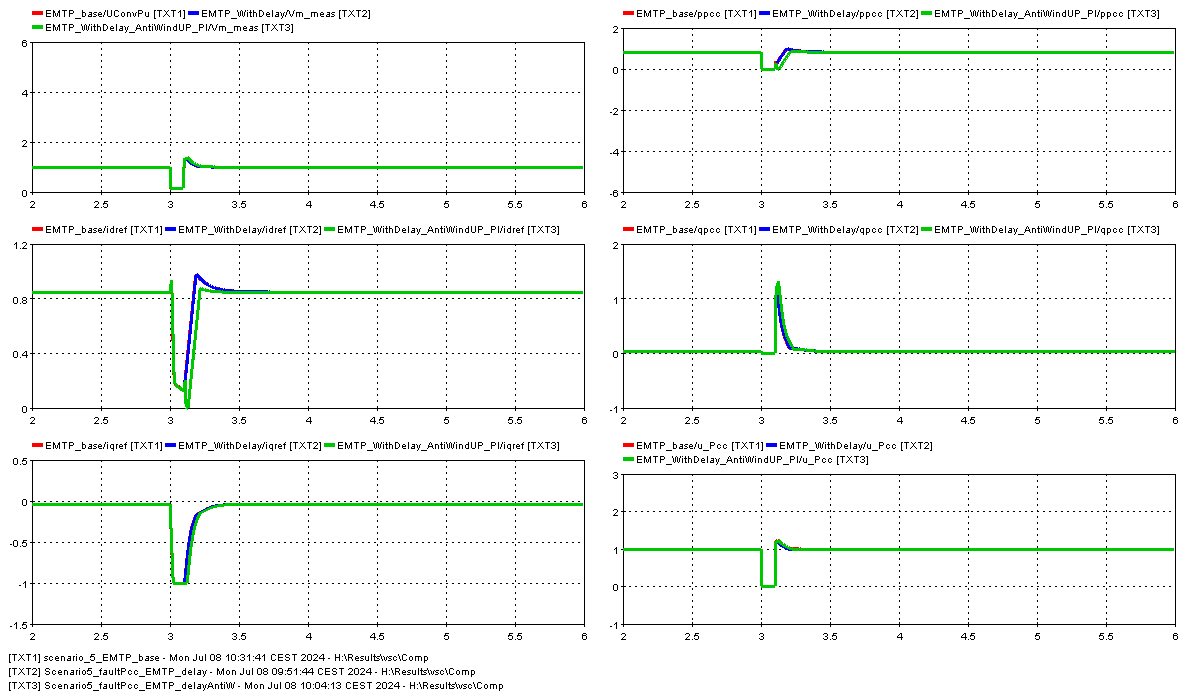
\includegraphics[scale = 0.4]{Figure_1VSC/CompEMTP.png}
  }
  \\
  \subfloat{
    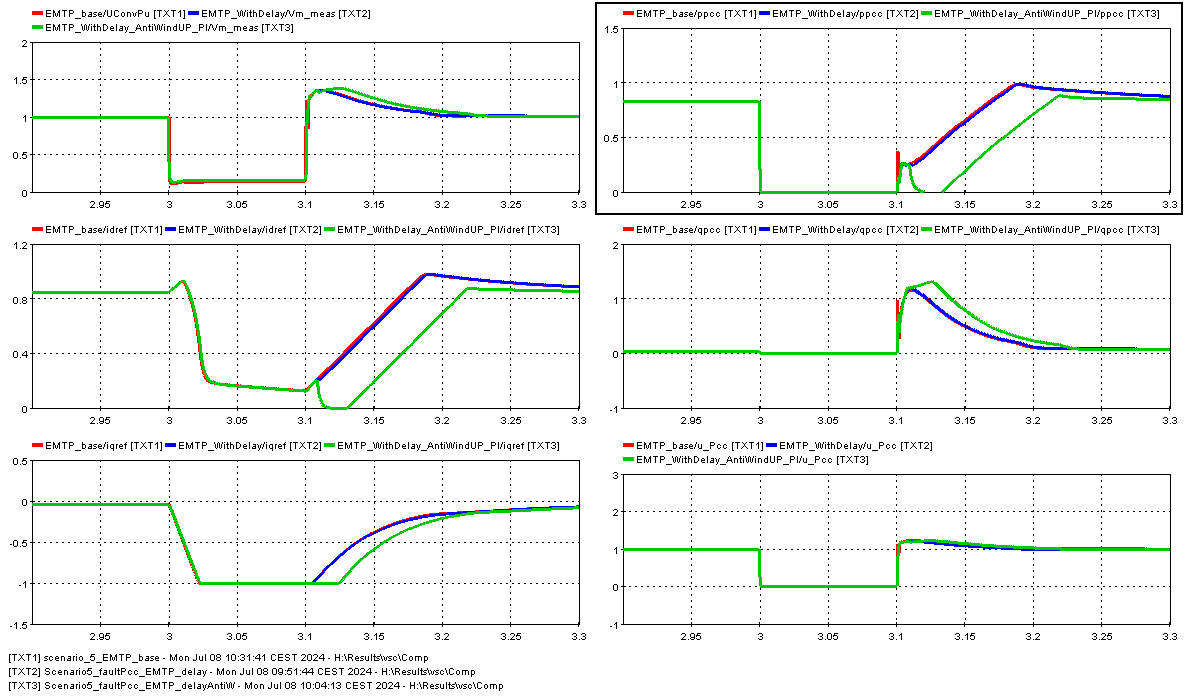
\includegraphics[scale = 0.4]{Figure_1VSC/CompEMTP_zoomed.png}
  }
  \caption{(a) Comparison of the reaction of $V_m$, $i_{{d,q}_{ref}}$, active (ppcc) and reactive power (qpcc) at PCC in (p.u.) and voltage at PCC of the modified 1 VSC models on fault at PCC (b) zoomed view. The solid red line denotes the responses of 1 VSC test system as previously modeled, solid blue line denotes the response of 1 VSC test system incorporates a low-pass filter for the measured signal of PCC voltage and current d-q components, along with a delay of $10^{-4}$ seconds when voltages are injected into the grid, and solid green line denotes The 1 VSC test system, similar to (2), includes anti-windup PI control for both the active power control loop and the reactive power control/voltage control loop.}
\label{fig:1VSC_Comp}
\end{figure}

\chapter{4-VSC test system - Converter-driven stability}
Power-electronics converters push the RMS simulation to its limit. Therefore, there is a need for benchmark systems with large penetration of converters. In this chapter, we present a 100\% converter-based test system: 4-VSC test system. This benchmark system is useful for evaluating, assessing, detecting, and mitigating converter-driven instability, particularly focusing on oscillation damping of specific system configurations and events. This benchmark was originally proposed by Prof. Thierry Van Cutsem (formerly with University of Liège, Belgium, acting as consultant for CRESYM). The VSC dynamic model was developed and validated by the team of Prof. Xavier Guillaud (Ecole Centrale de Lille, France). As part of the BiGER project (CRESYM), this test system has been implemented in Dynawo and EMTP.

\section{Test system description}
\subsection{Network description}
This 100\% power electronics small test system relies on Voltage Source Converters (VSC) operating in grid following mode. It aims at showing the limitations of RMS. The system was designed to offer the following features:\begin{itemize}
    \item Small enough to be easily tractable and for its stability margins to be easily assessed
    \item Complex enough to reflect real-life systems
    \item Involving several VSCs electrically rather close to each other (to contemplate possible interactions)
    \item  Being connected to an external grid of adjustable strength in terms of short-circuit power
    \item  Relying on generic models
    \item  Freely available \cite{colib}
\end{itemize}

The system hosts two wind parks (WP1 and WP2) and the terminal converters of two HVDC links (HVDC1 and HVDC2). The remote converter of each HVDC link is not modelled, the DC voltage being assumed constant. WP1 and WP2 are aggregated equivalents of a large number of generators. The connection transformers of all four VSCs are represented explicitly.

The connection to an external system is considered through the Thevenin equivalent attached to bus C. Since the Thevenin voltage source forces the system frequency to return to its nominal value in steady state, this 100\% power-electronics based system is clearly not meant to address frequency issues.
The 400-kV part of the transmission grid is meshed, allowing to simulate the outage of one or two circuits without disconnection from the external system. The line lengths are given in Table \ref{4-VSC_line_params}. Each wind park is radially connected to the grid through six 225-kV cables and six transformers in parallel to cope with the maximum production of each park. The cables are 50 km long and correspond to the AC connection of an offshore wind farm. The shunt reactors at buses E and F aim at absorbing the excess reactive power produced by the cables. The line, cable, transformer and VSC parameters are given in Table \ref{4-VSC_line_params}, \ref{4-VSC_trafo_params} and \ref{4-VSC_conv_params} , respectively.

\begin{table}[H]
\centering
\caption{4-VSC test system, line parameters}
\label{4-VSC_line_params}
\begin{tabular}{ccccccc}
\multicolumn{1}{c|}{\begin{tabular}[c]{@{}c@{}}line /\\ cable\end{tabular}} & \multicolumn{1}{c|}{\begin{tabular}[c]{@{}c@{}}nominal\\ voltage\end{tabular}} & \multicolumn{1}{c|}{\begin{tabular}[c]{@{}c@{}}R\\ ($\Omega$)\end{tabular}} & \multicolumn{1}{c|}{\begin{tabular}[c]{@{}c@{}}X\\ ($\Omega$)\end{tabular}} & \multicolumn{1}{c|}{\begin{tabular}[c]{@{}c@{}}$\omega$C/2\\ $\mu S$)\end{tabular}} & \multicolumn{1}{c|}{\begin{tabular}[c]{@{}c@{}}length\\ (km)\end{tabular}} & \begin{tabular}[c]{@{}c@{}}Snom\\ (MVA)\end{tabular} \\ \hline
\multicolumn{1}{c|}{A-C *}                                                  & \multicolumn{1}{c|}{400}                                                       & \multicolumn{1}{c|}{1.04}                                                   & \multicolumn{1}{c|}{20.80}                                                  & \multicolumn{1}{c|}{98}                                                             & \multicolumn{1}{c|}{65}                                                    & 3000                                                 \\
\multicolumn{1}{c|}{A-B *}                                                  & \multicolumn{1}{c|}{400}                                                       & \multicolumn{1}{c|}{0.51}                                                   & \multicolumn{1}{c|}{10.24}                                                  & \multicolumn{1}{c|}{48}                                                             & \multicolumn{1}{c|}{32}                                                    & 3000                                                 \\
\multicolumn{1}{c|}{B-C *}                                                  & \multicolumn{1}{c|}{400}                                                       & \multicolumn{1}{c|}{1.12}                                                   & \multicolumn{1}{c|}{22.40}                                                  & \multicolumn{1}{c|}{105}                                                            & \multicolumn{1}{c|}{70}                                                    & 3000                                                 \\
\multicolumn{1}{c|}{A2-E **}                                                & \multicolumn{1}{c|}{225}                                                       & \multicolumn{1}{c|}{0.42}                                                   & \multicolumn{1}{c|}{0.83}                                                   & \multicolumn{1}{c|}{9000}                                                           & \multicolumn{1}{c|}{50}                                                    & 2400                                                 \\
\multicolumn{1}{c|}{B2-F **}                                                & \multicolumn{1}{c|}{225}                                                       & \multicolumn{1}{c|}{0.42}                                                   & \multicolumn{1}{c|}{0.83}                                                   & \multicolumn{1}{c|}{9000}                                                           & \multicolumn{1}{c|}{50}                                                    & 2400                                                 \\
\multicolumn{7}{l}{* data of a single circuit}                                                                                                                 \\
\multicolumn{7}{l}{** data of 6 cables in parallel (400 MVA each)}                                                                                         
\end{tabular}
\end{table}

\begin{table}[H]
\centering
\caption{4-VSC test system, transformer parameters}
\label{4-VSC_trafo_params}
\begin{tabular}{cccccc}
\multicolumn{1}{c|}{transfomer} & \multicolumn{1}{c|}{\begin{tabular}[c]{@{}c@{}}nominal\\ voltages\end{tabular}} & \multicolumn{1}{c|}{\begin{tabular}[c]{@{}c@{}}R\\ (\%)\end{tabular}} & \multicolumn{1}{c|}{\begin{tabular}[c]{@{}c@{}}X\\ (\%)\end{tabular}} & \multicolumn{1}{c|}{\begin{tabular}[c]{@{}c@{}}transfo\\ ratio (\%)\end{tabular}} & \begin{tabular}[c]{@{}c@{}}Snom\\ (MVA)\end{tabular} \\ \hline
\multicolumn{1}{c|}{A1-A}       & \multicolumn{1}{c|}{320/400}                                                    & \multicolumn{1}{c|}{0.5}                                              & \multicolumn{1}{c|}{15.0}                                             & \multicolumn{1}{c|}{102.}                                                         & 1200                                                 \\
\multicolumn{1}{c|}{B1-B}       & \multicolumn{1}{c|}{320/400}                                                    & \multicolumn{1}{c|}{0.5}                                              & \multicolumn{1}{c|}{15.0}                                             & \multicolumn{1}{c|}{104.}                                                         & 1700                                                 \\
\multicolumn{1}{c|}{A2-A}       & \multicolumn{1}{c|}{225/400}                                                    & \multicolumn{1}{c|}{0.5}                                              & \multicolumn{1}{c|}{15.0}                                             & \multicolumn{1}{c|}{102.}                                                         & 2400                                                 \\
\multicolumn{1}{c|}{B2-B}       & \multicolumn{1}{c|}{225/400}                                                    & \multicolumn{1}{c|}{0.5}                                              & \multicolumn{1}{c|}{15.0}                                             & \multicolumn{1}{c|}{105.}                                                         & 2400                                                 \\
\multicolumn{1}{c|}{WP1-E *}    & \multicolumn{1}{c|}{66/225}                                                     & \multicolumn{1}{c|}{0.5}                                              & \multicolumn{1}{c|}{12.0}                                             & \multicolumn{1}{c|}{105.}                                                         & 2400                                                 \\
\multicolumn{1}{c|}{WP2-F *}    & \multicolumn{1}{c|}{66/225}                                                     & \multicolumn{1}{c|}{0.5}                                              & \multicolumn{1}{c|}{12.0}                                             & \multicolumn{1}{c|}{104.}                                                         & 2400                                                 \\
\multicolumn{6}{l}{* 6 transformers in parallel, 400 MVA each}                                                                                                                                                                                                                                                                                                                                              
\end{tabular}
\end{table}

\begin{table}[H]
\centering
\caption{4-VSC test system, converter parameters}
\label{4-VSC_conv_params}
\begin{tabular}{l|c|c}
\multicolumn{1}{c|}{Converter} & Snom (MVA) & Pnom (MW) \\ \hline
WP1                            & 2400       & 2300      \\
WP2                            & 2400       & 2300      \\
HVDC1                          & 1200       & 1150      \\
HVDC2                          & 1700       & 1630     
\end{tabular}
\end{table}

\subsection{Operating points}
Two operating points were considered in the simulations, as described in Table:

\begin{table}[H]
\centering
\begin{tabular}{l|cccc|c|c|c}
\begin{tabular}[c]{@{}l@{}}Operating \\ point \#\end{tabular} & \multicolumn{4}{c|}{\begin{tabular}[c]{@{}c@{}}Power (MW) \\ injected by\end{tabular}}     & \begin{tabular}[c]{@{}c@{}}power (MW) \\ into equiv.\end{tabular} & \begin{tabular}[c]{@{}c@{}}load (MW) \\ at bus C\end{tabular} & \begin{tabular}[c]{@{}c@{}}power (Mvar) \\ of shunt reactors\end{tabular} \\ \hline
                                                              & \multicolumn{1}{c|}{WP1}  & \multicolumn{1}{c|}{WP2}  & \multicolumn{1}{c|}{HVDC1} & HVDC2 & \multicolumn{1}{l|}{}                                             & \multicolumn{1}{l|}{}                                         & \multicolumn{1}{l}{}                                                      \\ \cline{2-5}
\multicolumn{1}{c|}{1}                                        & \multicolumn{1}{c|}{2000} & \multicolumn{1}{c|}{2000} & \multicolumn{1}{c|}{1150}  & 1400  & 6374                                                              & 0                                                             & 160                                                                       \\
\multicolumn{1}{c|}{2}                                        & \multicolumn{1}{c|}{2000} & \multicolumn{1}{c|}{2000} & \multicolumn{1}{c|}{-1120} & -1600 & 0                                                                 & 1169                                                          & 500                                                                      
\end{tabular}
\end{table}

Operating point 1:
The first operating conditions result in a heavily loaded network, both wind parks and both HVDC links injecting active power into the grid. Nevertheless, the system is N-1 secure with respect to the outage of any 400-kV circuit. No load is present. Hence, the whole production (minus the network losses) is exported to the external system represented by the Thévenin equivalent at bus C, whose short-circuit power has been set to 10 GVA. The operating point is shown in detail in Figure \ref{fig:4VSC_OP1}

% - Power injected by WPs and HVDC links
% - exported to external system
% - network heavily loaded
% - no load at external equivalent

\begin{figure}[H]
    \centering
    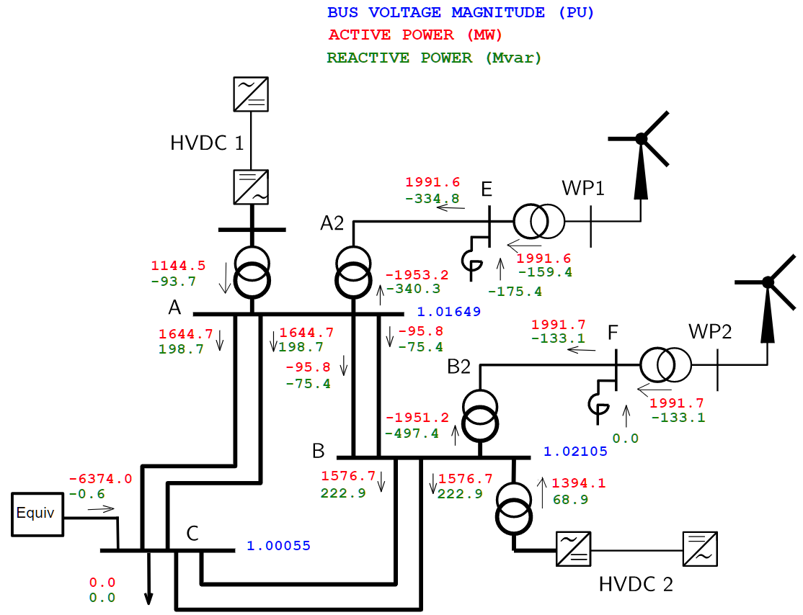
\includegraphics[scale = 0.6]{Figure_4VSC/4VSC_OP1.PNG}
    \caption{Operating point 1 of 4-VSC system}
    \label{fig:4VSC_OP1}
\end{figure}

Operating point 2:
In the second operating point, the wind parks inject the same power, a large fraction of which is evacuated by the HDVC links. This results in a lightly loaded network with larger shunt reactors connected. At this operating point, stability is assessed in terms of minimal short-circuit power of the external system. The corresponding Thévenin reactance is varied. The net power injection of the VSCs (minus the network losses) is taken by the load at bus C, which results in no power flowing into the Th´evenin equivalent. Hence, the initial state remains unchanged while the reactance is varied and there is no risk of reaching the (static) loadability limit of the equivalent (for large values of its reactance). The operating point is shown in detail in Figure \ref{fig:4VSC_OP2}.

\begin{figure}[H]
    \centering
    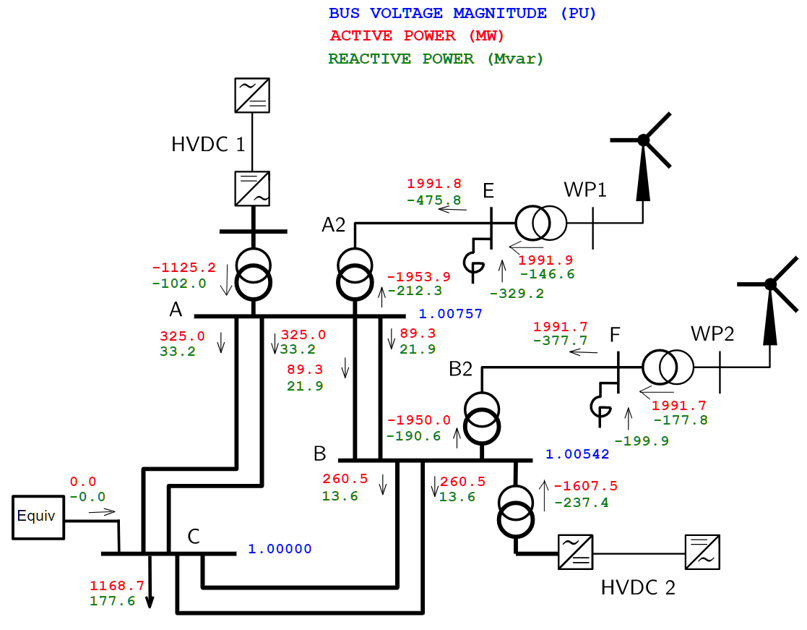
\includegraphics[scale = 0.6]{Figure_4VSC/4VSC_OP2.PNG}
    \caption{Operating point 2 of 4-VSC system}
    \label{fig:4VSC_OP2}
\end{figure}

The converter model parameters which are used in the 4-VSC test system are summarized in Table \ref{table_4VSC_model_parameters_OP2} and Table \ref{table_4VSC_model_parameters_OP1}.
\begin{table}[H]
\centering
\caption{4-VSC converters dynamic parameters, OP 1}
\begin{tabular}{ll|c|c|c|c}
\multicolumn{2}{l|}{}                                                  & HVDC 1    & HVDC 2    & WP 1      & WP 2      \\ \hline
\multicolumn{2}{l|}{Snom}                                              & 1200      & 1700      & 2400      & 2400      \\ \hline
\multicolumn{2}{l|}{P (MW)}                                            & 1144.5 & 1394.1   & 1991.6  & 1991.700  \\ \hline
\multicolumn{2}{l|}{Q (MVAr)}                                          & -53.7 & 504  & -159-4 & -736.8 \\ \hline
\multicolumn{2}{l|}{Vpcc (p.u.)}                                              & 1.016485  & 1.018446  & 1.068698  & 1.037386 \\ \hline
\multicolumn{2}{l|}{Angle - pcc (rad)}                                 &   0.210722        & 0.2166776           &    0.3523361       &   0.3664971         \\ \hline
\multicolumn{2}{l|}{Vconv (p.u.)}                                      & 1.024319  & 1.072794  & 1.069218  & 1.010584  \\ \hline
\multicolumn{2}{l|}{R (\%)}                                                 & 0.005     & 0.005     & 0.005     & 0.005     \\ \hline
\multicolumn{2}{l|}{L (\%)}                                                 & 0.15      & 0.15      & 0.12      & 0.12      \\ \hline
\multicolumn{1}{l|}{\multirow{2}{*}{Current loop}}        & Kp (p.u.)        & 0.5730    & 0.5730    & 0.4584    & 0.4584    \\ \cline{2-6} 
\multicolumn{1}{l|}{}                                     & Ki (pu/s)        & 6         & 6         & 6         & 6         \\ \hline
\multicolumn{1}{l|}{\multirow{6}{*}{Active power loop}}   & Tlpf (s)      & 0.0033    & 0.0033    & 0.0033    & 0.0033    \\ \cline{2-6} 
\multicolumn{1}{l|}{}                                     & Kpp (p.u.)       & 0.0333    & 0.0333    & 0.0333    & 0.0333    \\ \cline{2-6} 
\multicolumn{1}{l|}{}                                     & Kip (pu/s)       & 10        & 10        & 10        & 10        \\ \cline{2-6} 
\multicolumn{1}{l|}{}                                     & Trlim (s)     & 0.002     & 0.002     & 0.002     & 0.002     \\ \cline{2-6} 
\multicolumn{1}{l|}{}                                     & dP/dt\_min (pu/s) & -999      & -999      & -999      & -999      \\ \cline{2-6} 
\multicolumn{1}{l|}{}                                     & dP/dt\_max (pu/s) & 10        & 10        & 0.5       & 0.5       \\ \hline
\multicolumn{1}{l|}{\multirow{3}{*}{Reactive power loop}} & Kpv (p.u.)       & 0.1670    & 0.1670    & 0.0333    & 0.1670    \\ \cline{2-6} 
\multicolumn{1}{l|}{}                                     & Kiv (pu/s)       & 50        & 50        & 50        & 50        \\ \cline{2-6} 
\multicolumn{1}{l|}{}                                     & tau        & 0.1       & 0.1       & 0.1       & 0.1       \\ \hline
\multicolumn{1}{l|}{\multirow{2}{*}{PLL}}                 & Vpllb (p.u.)     & 0.4       & 0.4       & 0.4       & 0.4       \\ \cline{2-6} 
\multicolumn{1}{l|}{}                                     & Vpllu (p.u.)     & 0.5       & 0.5       & 0.5       & 0.5       \\ \hline
\multicolumn{2}{l|}{Imax (p.u.)}                                              & 1         & 1         & 1         & 1         \\ \hline
\multicolumn{2}{l|}{Vs1 (p.u.)}                                               & 0.95      & 0.95      & 0.95      & 0.95      \\ \hline
\multicolumn{2}{l|}{Vs2 (p.u.)}                                               & 0.5       & 0.5       & 0.5       & 0.5       \\ \hline
\multicolumn{2}{l|}{iqmax (p.u.)}                                             & 99        & 99        & 99        & 99       
\end{tabular}
\label{table_4VSC_model_parameters_OP1}
\end{table}

\begin{table}[H]
\centering
\caption{4-VSC converters dynamic parameters, OP 2}
\begin{tabular}{ll|c|c|c|c}
\multicolumn{2}{l|}{}                                                  & HVDC 1    & HVDC 2    & WP 1      & WP 2      \\ \hline
\multicolumn{2}{l|}{Snom}                                              & 1200      & 1700      & 2400      & 2400      \\ \hline
\multicolumn{2}{l|}{P (MW)}                                            & -1125.201 & -1607.5   & 1991.904  & 1991.700  \\ \hline
\multicolumn{2}{l|}{Q (MVAr)}                                          & -101.8893 & 346.1861  & -146.6046 & -783.3271 \\ \hline
\multicolumn{2}{l|}{Vpcc (p.u.)}                                              & 1.007573  & 1.005417  & 1.047555  & 0.9997311 \\ \hline
\multicolumn{2}{l|}{Angle - pcc (rad)}                                 &   0.0415856        & 0.0360115           &    0.18892       &   0.19649         \\ \hline
\multicolumn{2}{l|}{Vconv (p.u.)}                                      & 1.000011  & 1.040840  & 1.048864  & 0.970003  \\ \hline
\multicolumn{2}{l|}{R (\%)}                                                 & 0.005     & 0.005     & 0.005     & 0.005     \\ \hline
\multicolumn{2}{l|}{L (\%)}                                                 & 0.15      & 0.15      & 0.12      & 0.12      \\ \hline
\multicolumn{1}{l|}{\multirow{2}{*}{Current loop}}        & Kp (p.u.)        & 0.5730    & 0.5730    & 0.4584    & 0.4584    \\ \cline{2-6} 
\multicolumn{1}{l|}{}                                     & Ki (pu/s)        & 6         & 6         & 6         & 6         \\ \hline
\multicolumn{1}{l|}{\multirow{6}{*}{Active power loop}}   & Tlpf (s)      & 0.0033    & 0.0033    & 0.0033    & 0.0033    \\ \cline{2-6} 
\multicolumn{1}{l|}{}                                     & Kpp (p.u.)       & 0.0333    & 0.0333    & 0.0333    & 0.0333    \\ \cline{2-6} 
\multicolumn{1}{l|}{}                                     & Kip (pu/s)       & 10        & 10        & 10        & 10        \\ \cline{2-6} 
\multicolumn{1}{l|}{}                                     & Trlim (s)     & 0.002     & 0.002     & 0.002     & 0.002     \\ \cline{2-6} 
\multicolumn{1}{l|}{}                                     & dP/dt\_min (pu/s) & -999      & -999      & -999      & -999      \\ \cline{2-6} 
\multicolumn{1}{l|}{}                                     & dP/dt\_max (pu/s) & 10        & 10        & 0.5       & 0.5       \\ \hline
\multicolumn{1}{l|}{\multirow{3}{*}{Reactive power loop}} & Kpv (p.u.)       & 0.1670    & 0.1670    & 0.0333    & 0.1670    \\ \cline{2-6} 
\multicolumn{1}{l|}{}                                     & Kiv (pu/s)       & 50        & 50        & 50        & 50        \\ \cline{2-6} 
\multicolumn{1}{l|}{}                                     & tau        & 0.1       & 0.1       & 0.1       & 0.1       \\ \hline
\multicolumn{1}{l|}{\multirow{2}{*}{PLL}}                 & Vpllb (p.u.)     & 0.4       & 0.4       & 0.4       & 0.4       \\ \cline{2-6} 
\multicolumn{1}{l|}{}                                     & Vpllu (p.u.)     & 0.5       & 0.5       & 0.5       & 0.5       \\ \hline
\multicolumn{2}{l|}{Imax (p.u.)}                                              & 1         & 1         & 1         & 1         \\ \hline
\multicolumn{2}{l|}{Vs1 (p.u.)}                                               & 0.95      & 0.95      & 0.95      & 0.95      \\ \hline
\multicolumn{2}{l|}{Vs2 (p.u.)}                                               & 0.5       & 0.5       & 0.5       & 0.5       \\ \hline
\multicolumn{2}{l|}{iqmax (p.u.)}                                             & 99        & 99        & 99        & 99       
\end{tabular}
\label{table_4VSC_model_parameters_OP2}
\end{table}

\section{Implementations and validation results}
\subsection{Static simulation}
Static simulation often referred to as power flow or load flow analysis, is a fundamental technique used to determine the steady-state operating conditions of an electrical power system. It is a crucial step that serves as the initialization for dynamic simulations, particularly as the size of the network increases. This process allows for the investigation of different operating points within the power system. The challenge in implementation lies in converting network parameters such as transformers, transmission lines, and shunts between simulators, as each simulator follows its own conventions. Therefore, a crucial step after model exchange and comparison between simulators is validation. This validation is accomplished by comparing the results of load flow simulations. The tables \ref{static_OP1},  \ref{static_OP2} show the results of the static simulation in STEPSS (power flow module), Dynawo (dynaflow module), EMTP (power flow module)) for the two operating points 1 and 2. Table \ref{static_diff_OP1} and \ref{static_diff_OP2} show the error in Dynawo and EMTP with respect to STEPSS.

\begin{table}[H]
\centering
\caption{Comparaison of static simulation results between STEPSS, Dynawo and EMTP for Operating point 1}

\begin{tabular}{c|c c|c c|c c|c|} 
& STEPSS && Dynawo  && EMTP && \\ 
Bus & Vmag  & Vangle  & Vmag & Vangle &  Vmag & Vangle & \\ 
&   (p.u.) & (deg) &  (p.u.) & (deg) &  (p.u.) & (deg) &\\
\hline
A & 1.0164853 & 12.0734801 & 1.0164853 & 12.07352488 & 1.0164853 & 12.07248368 \\ 
A2 & 1.0509079 & 18.59682175 & 1.0509079 & 18.5968666 & 1.0477824 & 18.61866523 \\
B & 1.0184461 & 12.41471142 & 1.018445 & 12.41476747 & 1.0184461 & 12.41454252 \\
B2 & 1.0258986 & 19.13032682 & 1.0258984 & 19.13042386 & 1.0228409 & 19.15761283 \\
C & 1.00055 & 0 & 1.00055 & 0 & 1.00055 & 0 \\
E & 1.0686982 & 20.18737035 & 1.068698 & 20.18741514 & 1.0686982 & 20.12857984 \\
F & 1.0373857 & 20.99873933 & 1.0373857 & 20.99884582 & 1.0373857 & 20.9462333 \\ 
\end{tabular}
\label{static_OP1}
\end{table}
The difference in \% is shown in the following table:
\begin{table}[H]
\centering
\caption{Difference in \%, OP1}
\begin{tabular}{ll|ll}
\multicolumn{2}{c|}{Dynawo - STEPSS (\%)}                      & \multicolumn{2}{c}{EMTP - STEPSS (\%)}                        \\ \hline
\multicolumn{1}{c|}{Vmag}         & \multicolumn{1}{c|}{Angle} & \multicolumn{1}{c|}{Vmag}         & \multicolumn{1}{c}{Angle} \\ \hline
\multicolumn{1}{l|}{3.04912E-11}  & -0.000370854               & \multicolumn{1}{l|}{0.000000000}  & -0.008253003              \\
\multicolumn{1}{l|}{3.26988E-07}  & -0.000241464               & \multicolumn{1}{l|}{-0.297404384} & 0.117458118               \\
\multicolumn{1}{l|}{-1.53539E-05} & -0.000451486               & \multicolumn{1}{l|}{0.000000000}  & -0.001360499              \\
\multicolumn{1}{l|}{-1.24651E-05} & -0.000507273               & \multicolumn{1}{l|}{-0.298043353} & 0.142632218               \\
\multicolumn{1}{l|}{1.86795E-06}  & 0                          & \multicolumn{1}{l|}{0.000000000}  & \#DIV/0!                  \\
\multicolumn{1}{l|}{-4.76814E-06} & -0.00022186                & \multicolumn{1}{l|}{0.000000000}  & -0.291224232              \\
\multicolumn{1}{l|}{1.72665E-10}  & -0.000507156               & \multicolumn{1}{l|}{0.000000000}  & -0.250043704             
\end{tabular}
\label{static_diff_OP1}
\end{table}

\begin{table}[H]
\centering
\caption{Comparaison of static simulation results between STEPSS, Dynawo and EMTP for Operating point 2}

\begin{tabular}{c|c c|c c|c c|} 
& STEPSS && Dynawo  && EMTP &\\ 
Bus & Vmag  & Vangle  & Vmag & Vangle &  Vmag & Vangle \\ 
&   (p.u.) & (deg) &  (p.u.) & (deg) &  (p.u.) & (deg) \\
\hline
A & 1.0075727 & 2.382680113 & 1.0075727 & 2.38267631 & 1.0075727 & 2.383839362 \\ 
A2 & 1.0318668 & 9.103813496 & 1.03186678 & 9.103809461 & 1.0299952 & 9.129842945 \\
B & 1.0054174 & 2.063309084 & 1.0054174 & 2.063303753 & 1.0054174 & 2.065603698 \\
B2 & 0.9925507 & 9.119518843 & 0.9925506 & 9.119504417 & 0.9895866 & 9.153261338 \\
C & 1 & 0 & 1 & 0 & 1 & 0 \\
E & 1.0475551 & 10.82446191 & 1.047555 & 10.82445804 & 1.0475551 & 10.77026275 \\
F & 0.9997311 & 11.2583617 & 0.9997311 & 11.25834358 & 0.9997311 & 11.21313787 \\ 
\end{tabular}
\label{static_OP2}
\end{table}

The difference in \% for OP2 is shown in the following table:
\begin{table}[H]
\centering
\caption{Difference in \%, OP2}
\begin{tabular}{ll|ll}
\multicolumn{2}{c|}{Dynawo - STEPSS (\%)}                    & \multicolumn{2}{c}{EMTP - STEPSS (\%)}                        \\ \hline
\multicolumn{1}{c|}{Vmag}       & \multicolumn{1}{c|}{Angle} & \multicolumn{1}{c|}{Vmag}         & \multicolumn{1}{c}{Angle} \\ \hline
\multicolumn{1}{l|}{0.0000000}  & 0.000159643                & \multicolumn{1}{l|}{0.000000000}  & 0.048653138               \\
\multicolumn{1}{l|}{-0.0000019} & 4.43304E-05                & \multicolumn{1}{l|}{-0.297671409} & 0.285918078               \\
\multicolumn{1}{l|}{0.0000000}  & 0.000258345                & \multicolumn{1}{l|}{0.000000000}  & 0.111210392               \\
\multicolumn{1}{l|}{-0.0000020} & 0.000158188                & \multicolumn{1}{l|}{-0.298624787} & 0.370003024               \\
\multicolumn{1}{l|}{0.0000000}  & 0                          & \multicolumn{1}{l|}{0.000000000}  & 0                         \\
\multicolumn{1}{l|}{0.0000028}  & 3.57354E-05                & \multicolumn{1}{l|}{0.000000000}  & -0.500709925              \\
\multicolumn{1}{l|}{0.0000000}  & 0.000160898                & \multicolumn{1}{l|}{0.000000000}  & -0.401691015             
\end{tabular}
\label{static_diff_OP2}
\end{table}



\subsection{Dynamic simulation}
To trigger the dynamic simulation from the steady state operating point a mild and a severe disturbance are implemented. The mild disturbance is the opening of one circuit of the line between buses A and B. This 400-kV circuit carrying only 90 MW, the disturbance can be considered small; the purpose of the simulation is to test the small-disturbance stability of the resulting operating point.
The severe disturbance is a solid three-phase fault on one of the two circuits of line A-C, next to bus A. The fault is cleared after 100 ms by opening the line, which remains open. The purpose of the simulation is to test the response to a large disturbance leading to current limitation in the VSCs. Both events are tested for OP1 and OP2 and compared to each other for the three simulators STEPSS, dynawo and EMTP. The simulation results are presented in the next section.

\subsection{Simulation results}
The simulations settings of the different simulators are summarized in the following table:

\begin{table}[H]
\centering
\caption{4-VSC simulation settings}
\begin{tabular}{lccc}
\hline
                   & \textbf{STEPSS}                  & \textbf{Dynawo} & \textbf{EMTP} \\ \hline
Domain             & RMS                              & RMS             & EMT           \\ \hline
Duration           & 10s                              & 10s             & 10s           \\ \hline
Step size          & 1ms (fix)                        & 1ms (fix)       & 50us (fix)    \\ \hline
Solver             & DAE                              & DAE             & Nodal         \\ \hline
Integration method & BDF & BE  & Trapezoidal   \\ \hline
\end{tabular}
\label{4VSC_simulation_params}
\end{table}

The same GFL model is used for the 4-VSC system implementation in EMTP, as shown in \figurename~\ref{4VSC_system_EMTP}. It consists of four GLF converters, HVDC1 is connected to bus A and HVDC2 to bus B. There are also two wind power plants, where WP1 is connected to bus E, and WP2 to bus F.
\begin{figure}[H]
    \centering
    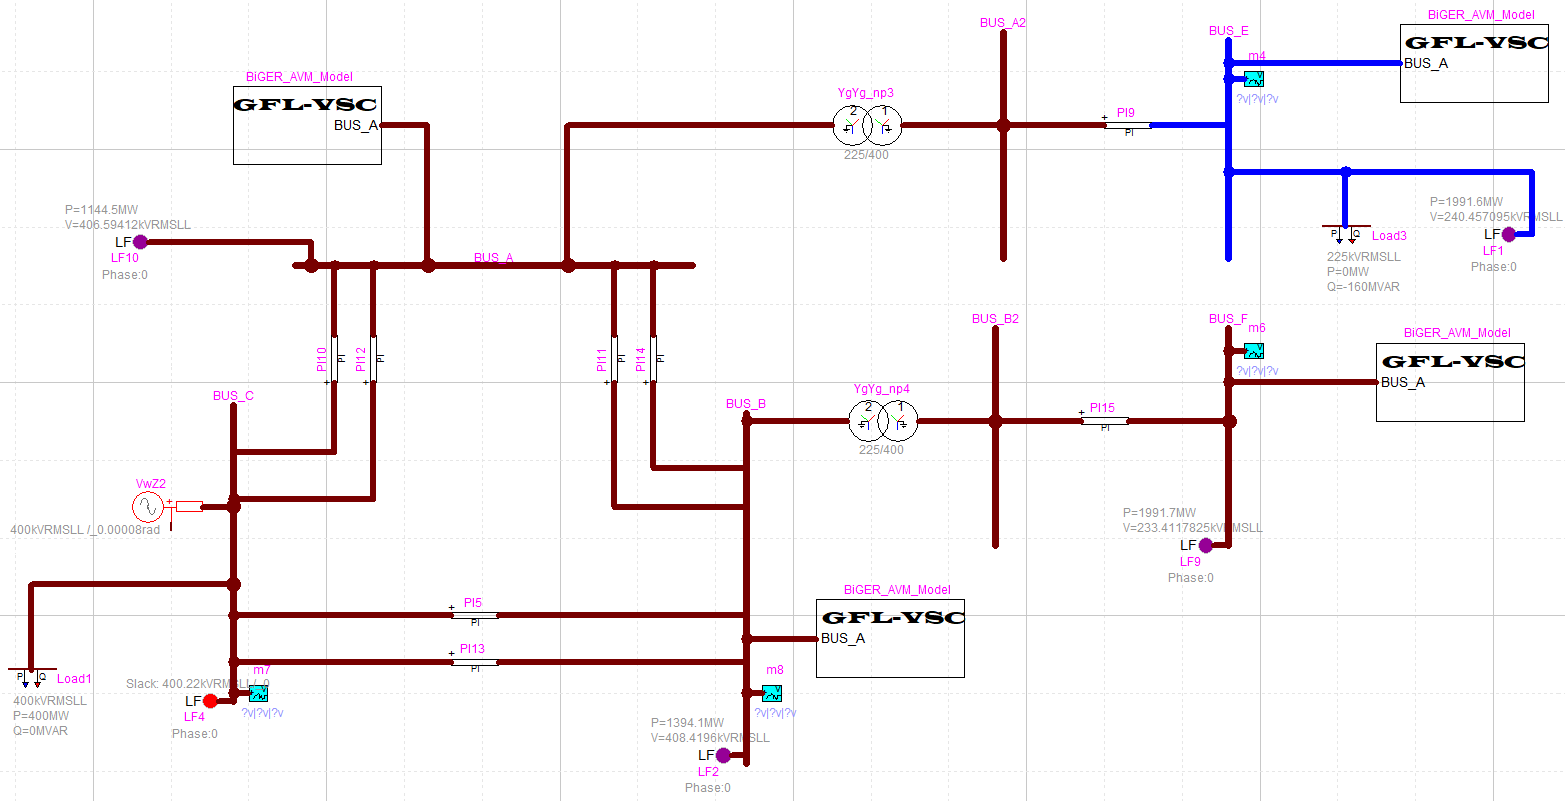
\includegraphics[scale = 0.4]{Figure_4VSC/4VSC_system_EMTP.png}
    \caption{4-VSC system - EMTP}
    \label{4VSC_system_EMTP}
\end{figure}

As described above, to compare the dynamic simulation results obtained by different software, a fault and line disconnection are performed for both operating points, and again \eqref{sine_to_RMS} is used to translate the values from the EMT simulation to RMS values. As previously described, two operating points are considered and simulated. 
The Figures show the evolution of the voltages at different locations.

\begin{figure}[H]
    \centering
    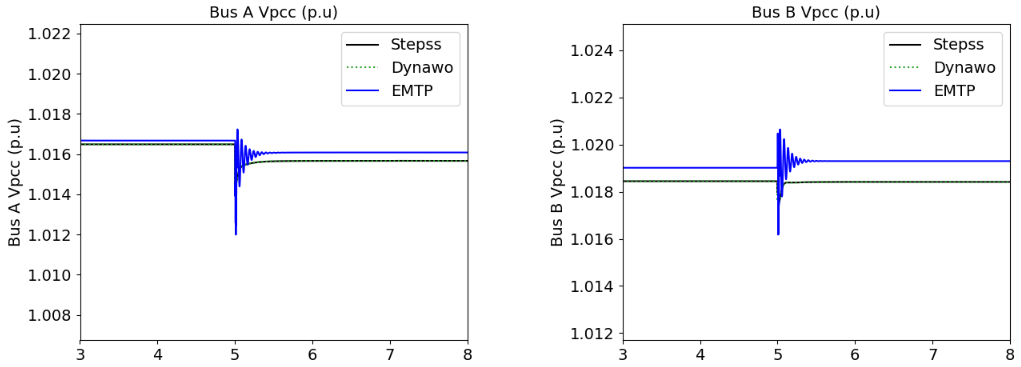
\includegraphics[width = \columnwidth]{Figure_4VSC/4VSC_OP1_line_disconnect.png}
    \caption{4-VSC system, line disconnect A-B, OP1}
    \label{fig:4VSC_line_disconnect_OP1}
\end{figure}
\begin{figure}[H]
    \centering
    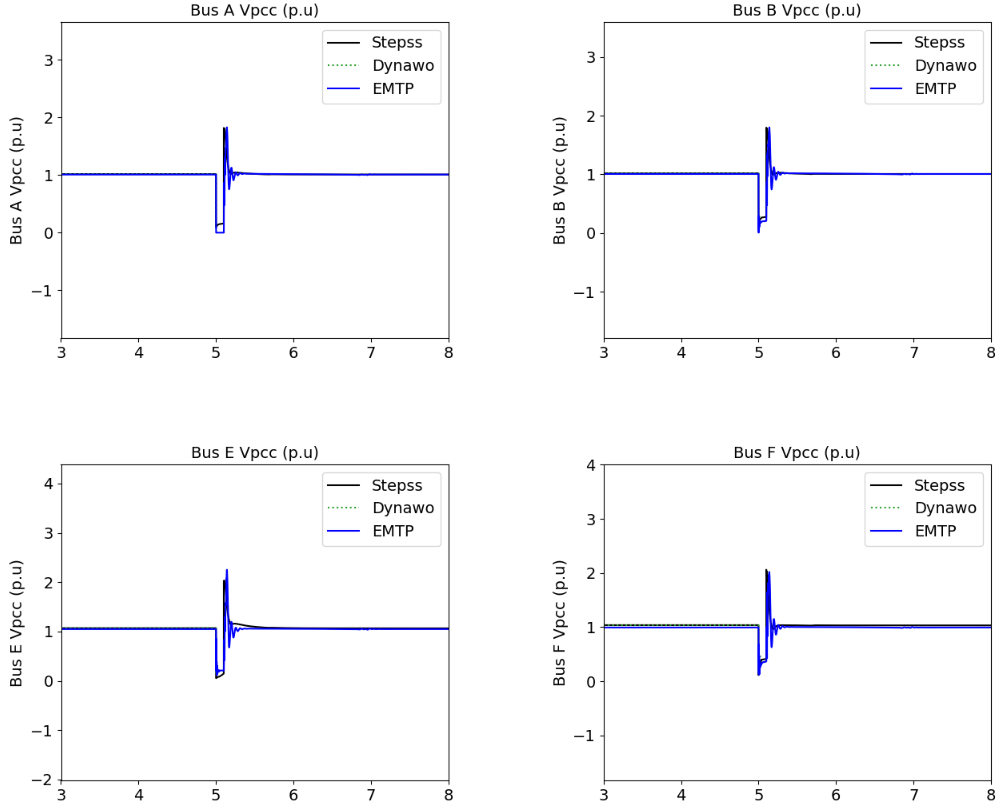
\includegraphics[width = \columnwidth]{Figure_4VSC/4VSC_OP1_fault.png}
    \caption{4-VSC system, fault A, OP1}
    \label{fig:4VSC_fault_OP1}
\end{figure}
\begin{figure}[H]
    \centering
    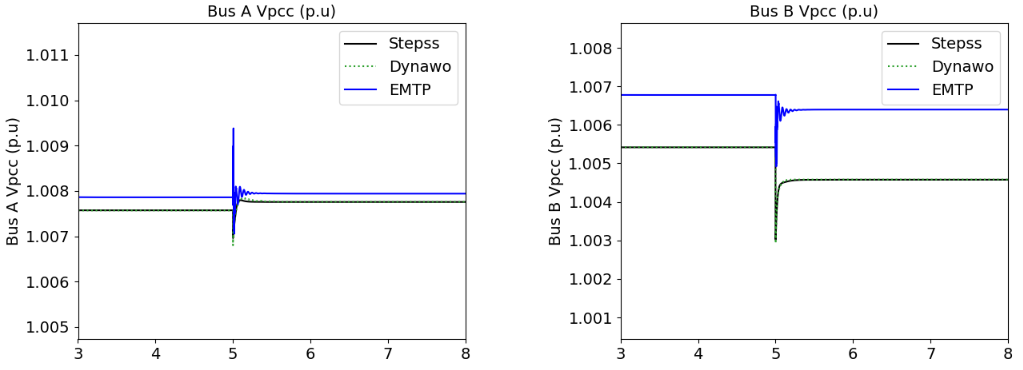
\includegraphics[width = \columnwidth]{Figure_4VSC/4VSC_OP2_line_disconnect.png}
    \caption{4-VSC system, line disconnect A-B, OP2}
    \label{fig:4VSC_line_disconnect_OP2}
\end{figure}
\begin{figure}[H]
    \centering
    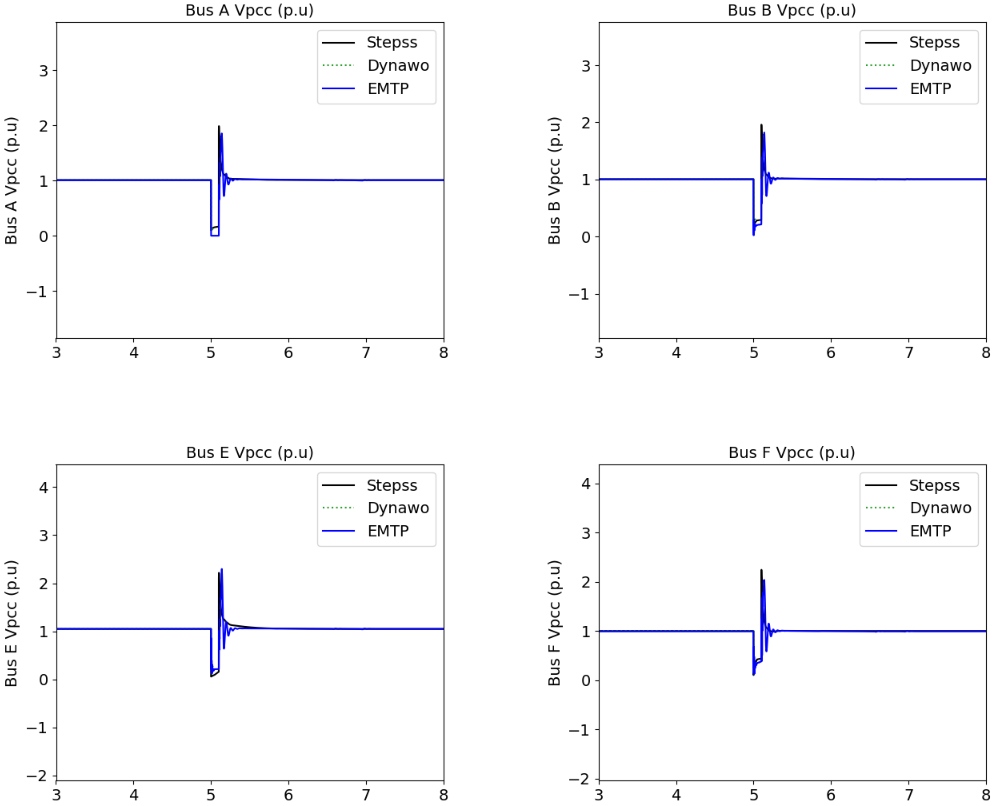
\includegraphics[width = \columnwidth]{Figure_4VSC/4VSC_OP2_fault.png}
    \caption{4-VSC system, fault A, OP2}
    \label{fig:4VSC_fault_OP2}
\end{figure}

The steady-state values after the fault and line disconnect are presented in Table \ref{table_4VSC_results_fault_line_disconnect}
\begin{table}[H]
\centering
\caption{Steady-state values after the transient}
\begin{tabular}{ll|c|c|c|c|}
                                                        &        & \multicolumn{1}{c|}{\begin{tabular}[c]{@{}c@{}}OP1\\ Line disconnet\end{tabular}} & \multicolumn{1}{c|}{\begin{tabular}[c]{@{}c@{}}OP1\\ Fault\end{tabular}} & \multicolumn{1}{c|}{\begin{tabular}[c]{@{}c@{}}OP 2\\ Line disconnect\end{tabular}} & \multicolumn{1}{c|}{\begin{tabular}[c]{@{}c@{}}OP 2\\ Fault\end{tabular}} \\ \hline
\multicolumn{1}{l|}{\multirow{3}{*}{Bus A Vpcc (p.u.)}} & STEPSS & 1.01566                                                                           & 1.00899                                                                  & 1.00776                                                                             & 1.00769                                                                   \\
\multicolumn{1}{l|}{}                                   & Dynawo & 1.01566                                                                           & 1.00865                                                                      & 1.00776                                                                             & 1.00766                                                                       \\
\multicolumn{1}{l|}{}                                   & EMTP   & 1.01608                                                                           & 1.00786                                                                  & 1.00794                                                                             & 1.00531                                                                   \\ \hline
\multicolumn{1}{l|}{\multirow{3}{*}{Bus B Vpcc (p.u.)}} & STEPSS & 1.01842                                                                           & 1.00714                                                                  & 1.00458                                                                             & 1.00486                                                                   \\
\multicolumn{1}{l|}{}                                   & Dynawo & 1.01842                                                                           & 1.00714                                                                      & 1.00458                                                                             & 1.00488                                                                       \\
\multicolumn{1}{l|}{}                                   & EMTP   & 1.01929                                                                           & 1.00678                                                                  & 1.00639                                                                             & 1.00205                                                                   \\ \hline
\multicolumn{1}{l|}{\multirow{3}{*}{Bus E Vpcc (p.u.)}} & STEPSS & -                                                                                 & 1.06571                                                                  & 1.04763                                                                             & 1.04761                                                                   \\
\multicolumn{1}{l|}{}                                   & Dynawo & -                                                                                 & 1.06572                                                                      & 1.04763                                                                             & 1.04763                                                                       \\
\multicolumn{1}{l|}{}                                   & EMTP   & -                                                                                  & 1.04952                                                                  & 1.04954                                                                             & 1.04850                                                                   \\ \hline
\multicolumn{1}{l|}{\multirow{3}{*}{Bus F Vpcc (p.u.)}} & STEPSS & -                                                                                 & 1.03284                                                                  & 0.99939                                                                             & 0.99951                                                                   \\
\multicolumn{1}{l|}{}                                   & Dynawo & -                                                                                 & 1.03284                                                                      & 0.99939                                                                             & 0.99952                                                                       \\
\multicolumn{1}{l|}{}                                   & EMTP   & -                                                                                 & 0.99381                                                                  & 0.99365                                                                             & 0.99193                                                                  
\end{tabular}
\label{table_4VSC_results_fault_line_disconnect}
\end{table}
The results align closely, with any potential differences being so small that they are effectively insignificant (maximum around 1kV). This minor variation does not impact the overall conclusions, ensuring that the findings remain reliable.

\section{Example Study: stability limit as function of External Network Strength}
In this section, we present an initial example of a stability analysis conducted with the implemented 4-VSC system that shows significant differences between RMS and EMT simulations. The simulations consist of a mild disturbance (line disconnection) for OP1 and OP2 in the three simulators STEPSS, Dynawo and EMTP.
In order to find the stability limit of the system, starting from a 20000MVA the short-circuit power of the external system (connected to bus C) is progressively decreased in 500MVA steps, until the response to the disturbance becomes unacceptable, owing to undamped oscillations. The stability limit is identified as the last value where all bus voltage oscillations are damped and the system regains it's steady state value after the disturbance is removed. The limit value of the short-circuit power obtained with respectively EMT and RMS simulations have been compared between STEPSS, Dynawo and EMTP. The results of this analysis are reported in Table \ref{table_4VSC_SCR}. In addition, the evolution of the voltage at Bus C is shown in Figure \ref{fig:SCR_OP1} and \ref{fig:SCR_OP2} for OP1 and OP2 respectively for the stable, marginally stable and unstable cases.

\begin{table}[H]
\caption{Stability short circuit power limits}
\centering
\begin{tabular}{|c|cc|}
\hline
\multicolumn{1}{|c|}{}          & \multicolumn{2}{c|}{\textbf{Short circuit power (MVA)}}                       \\ \hline
\multicolumn{1}{|c|}{\textbf{}} & \multicolumn{1}{c|}{\textbf{OP1}} & \multicolumn{1}{c|}{\textbf{OP2}} \\ \hline
\textbf{STEPSS}                 & \multicolumn{1}{c|}{3900}        & \multicolumn{1}{c|}{2400}            \\ \hline
\textbf{Dynawo}                 & \multicolumn{1}{c|}{4000}        & \multicolumn{1}{c|}{3850}                                   \\ \hline
\textbf{EMTP}                   & \multicolumn{1}{c|}{13500}       & \multicolumn{1}{c|}{12500}                                  \\ \hline
\end{tabular}
\label{table_4VSC_SCR}
\end{table}

\begin{figure}[H]
    \centering

  \subfloat[]{
    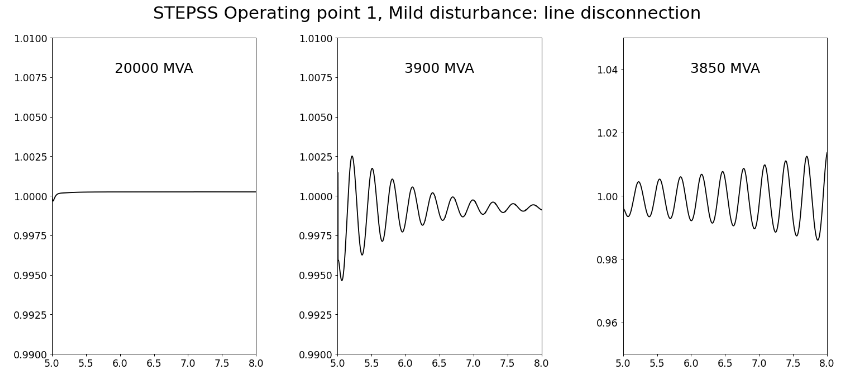
\includegraphics[scale = 0.6]{Figure_4VSC/SCR_STEPSS_OP1.PNG}
  }

 \subfloat[]{
    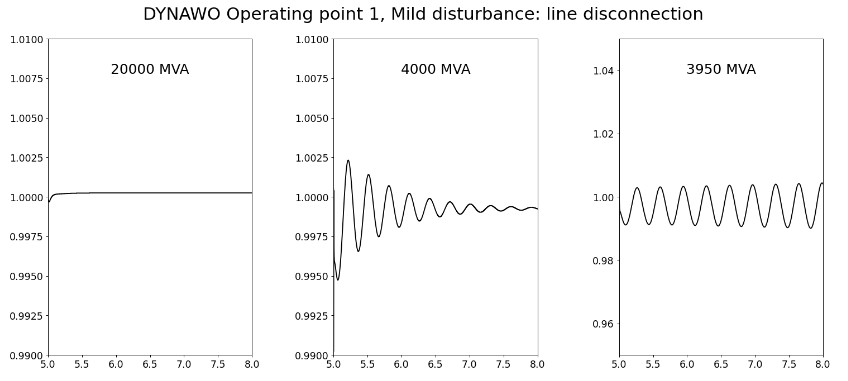
\includegraphics[scale = 0.6]{Figure_4VSC/SCR_DYNAWO_OP1.PNG}
  }

\subfloat[]{
    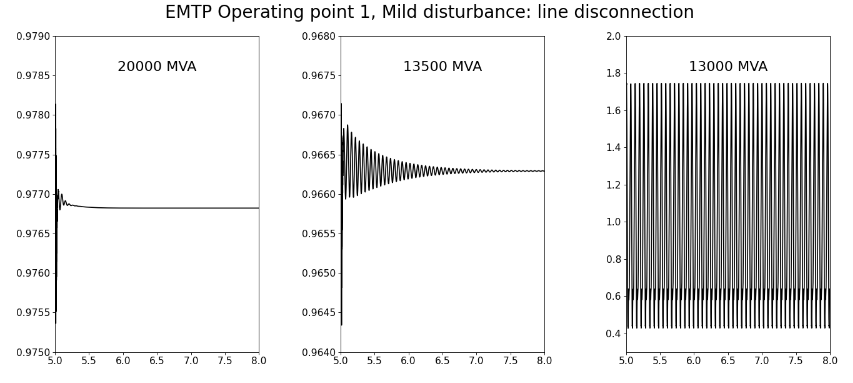
\includegraphics[scale = 0.6]{Figure_4VSC/SCR_EMTP_OP1.PNG}
  }

\caption{}
\label{fig:SCR_OP1}
\end{figure}


\begin{figure}[H]
    \centering

  \subfloat[]{
    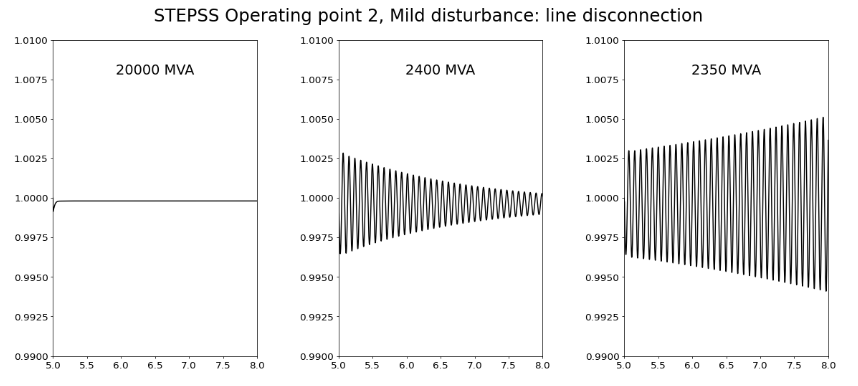
\includegraphics[scale = 0.6]{Figure_4VSC/SCR_STEPSS_OP2.PNG}
  }

 \subfloat[]{
    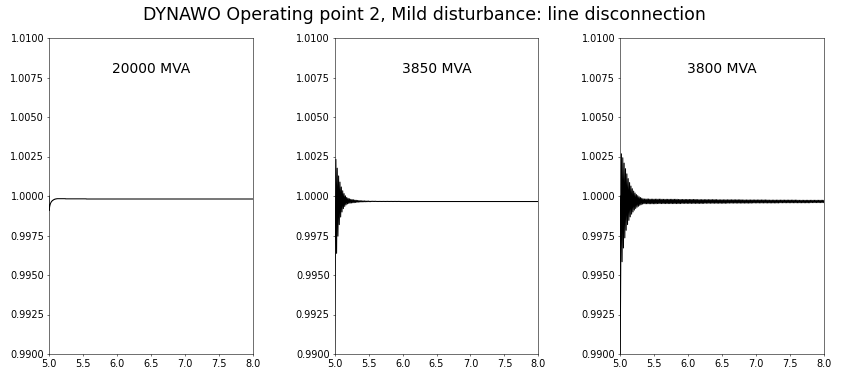
\includegraphics[scale = 0.6]{Figure_4VSC/SCR_DYNAWO_OP2.PNG}
  }

\subfloat[]{
    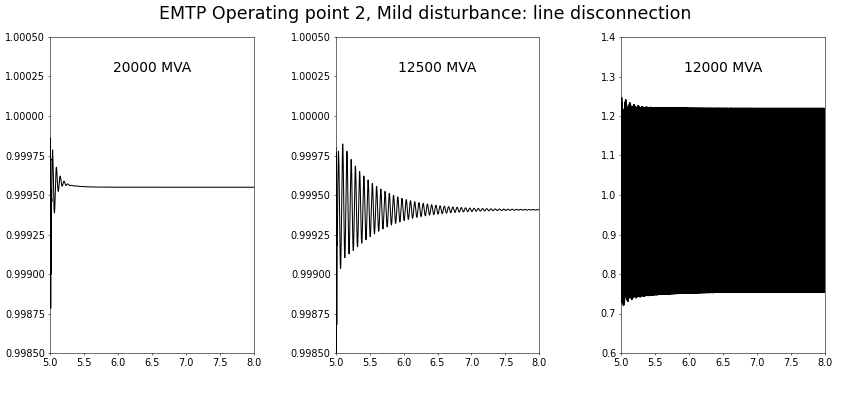
\includegraphics[scale = 0.6]{Figure_4VSC/SCR_EMTP_OP2.PNG}
  }

\caption{}
\label{fig:SCR_OP2}
\end{figure}

\newpage
 

As presented in Table \ref{table_4VSC_SCR}, there are significant discrepancies between RMS and EMT in terms of stability limits. It can be seen that in EMT simulations the system becomes unstable for a short-circuit power ranging from 12.5GVA to 13.5GVA, while in RMS simulations becomes unacceptable for a short-circuit power ranging from 2.4GVA to 4GVA. There is thus a very significant difference by a factor of 3. Furthermore, the differences between the two RMS simulators depend on the operating point, with a difference of 0.1GVA for OP1 and 1.45GVA for OP2. Thus, these discrepancies become more pronounced for OP2 with the lightly loaded network. Additionally, for all simulators, higher frequency voltage waveforms are observed for OP2 compared to OP1. The high-frequency oscillations observed in Dynawo for OP2 when approaching the stability limit are related to the solver configuration. These oscillations can be altered by adjusting the solver parameters. This aspect requires further investigation.

%%%%%%%%%%%%%%%%%%%%%%%%%%%%%%%%%%%%%%%%%%%%%%%%%%%%%%%%%%%%%%%%%%%%%%%%%%%%%%%%%%%%%%%%%%%%%%%%%%%%%%%%%%%%%%%%%%%%%%%%%%%%%%%%%%%%%%%%%%%%%%%%%%%%
\chapter{Nordic test system - Short-term voltage
stability}
This chapter aims to set up a test system in which synchronous generators are still dominating. The Nordic test system adapts the well-documented benchmark system \cite{van2015test} for Electromagnetic Transient (EMT) simulations, enabling comparisons with phasor-mode simulations. This benchmark system offers a model for evaluating new solutions for assessing, detecting, and mitigating voltage instability, particularly focusing on long-term voltage instability that leads to collapse typically a few minutes after the initiating events, approximately 90 seconds. Load tap changers and field current limiters drive those dynamics. To align the Nordic system with the current stability definition, which encompasses more converter-interfaced generations, the report EMT-phasor comparison is not limited to the fast dynamics of VSCs. Therefore, the focus is shifted from long-term to short-term dynamics\cite{hatziargyriou2020definition}. This shift is accomplished by replacing a subset of synchronous generators with Voltage Source Converters (VSCs). The Nordic test system models a real power system scenario where synchronous generators (SGs) and VSCs coexist. The Nordic test system, with Operating Point A, which is not N-1 secure for several contingencies, is considered.

\section{Test system description}
An overall description of the Nordic system is provided in Table \ref{table:1} and \ref{System Descriptions Area Wise}. The main system structure has long transmission lines with 400-kV nominal voltage. Some regional systems operate at 220 and 130 kV. The generator bus voltage level is 15 KV, stepped up and connected to the transmission system. A step-down transformer connects the load bus to 20 KV. Generator G20 is considered a slack bus. The details of the exciter, turbine, and generator are specified in \cite{van2015test} and later in the chapter. The stator resistance of the machines is set to zero in all generators. Hence, the power produced by the machine is equal to the mechanical power received from the prime mover. In other words, the mechanical power is equal to the power specified (or calculated, at the slack bus) in the power flow data.
\begin{table}[h!]
\centering
\caption{Test Model: Nodic System Detail}
\begin{tabular}{|c|c|}
 \hline
 \hline
 Nominal frequency & 50 Hz \\
 \hline
 Number of Buses & 74 \\
 \hline
 Number of lines & 50 \\
 \hline
 Number of transformers & 52 \\ 
  \hline
 Number of Generators & 19 -represented behind their step-up transformers\\
   \hline
 Number of Synchronous Condenser & 1 -represented behind their step-up transformers\\
 \hline
  Number of loads & 22 22 at distribution level \\ 
  \hline
   Number of (switched) shunts & 11 \\ 
     \hline
   Total Generation & 11506 MW \\   \hline
   Total load & 11060 MW \\ 
  \hline
 \hline
\end{tabular}
\label{table:1}
\end{table}
The Nordic system is divided into four areas, a description of which is mentioned in Table \ref{System Descriptions Area Wise}. The system is modeled in in EMTP with simulation options: Numerical Integration Method- Trapezoidal and Backward Euler, and Time domain solution- Main time step ($\Delta t$)= 50 $\mu s$
\begin{table}[h!]
\centering
\caption{System Descriptions Areawise}
\begin{tabular}{|c|c|c|}
 \hline
 \textbf{Area}  & \textbf{Generation } & \textbf{Load}\\
  \textbf{}  & \textbf{(MW)} & \textbf{(MW)}\\
 \hline
 North with hydro generation and some load.
 & 4629 & 1180 \\
  Generators are equipped with governor control & & \\
 \hline
 Central with much higher load and thermal power generation.
& 2850 & 6190\\
 \hline
South with the thermal generation, 
 & 1590 & 1390 \\
  which is rather loosely connected to the rest of the system. & & \\
 \hline
 Equivalent is connected to the “North”, which includes a simple   &
 2437 & 2300\\
 equivalent of external system. Generators are equipped with governor control &  & \\
 \hline
 \hline
\end{tabular}
\label{System Descriptions Area Wise}
\end{table}

\subsection{Implementation choice-Conventional Nordic System}
To accurately model the Nordic System in the EMTP Simulator, the following test systems are implemented step by step.
\begin{itemize}
    \item[I.]  Nordic system with generator as AC Voltage Source for Load Flow Analysis.
    \item[II.]  Single machine infinite bus (SMIB) for testing Nordic system generators response.
    \item[III.]  Small test system with two detailed generators to verify the turbine, governor, and exciter response. 
    \item[IV.]  Full detailed Nordic system.
\end{itemize}


 %\textbf{Comparison of EMTP and STEPSS Simulations: With and Without Machine Saturation}
 %Machine saturation describes the non-linear behavior of magnetic materials in electrical machines under high magnetic flux densities. Incorporating machine saturation impacts simulation results in the following ways:
%\subsubsection{Model assumptions}
%\textit{Linear model assumption without machine saturation:} assume a linear relationship between the magnetic flux and the magnetizing current. This simplification leads to more predictable and less complex simulation results. Linear and proportional response characteristics such as voltage, current, and magnetic flux.
%\textit{Non-linear Model with Machine Saturation:} incorporating machine saturation introduces non-linear characteristics, resulting in a more realistic simulation. Non-linear relationship between magnetic flux and magnetizing current, especially at higher flux densities. 
%\subsubsection{Transient Stability}
%\textit{Transient stability without machine saturation:} provides a faster and more idealized transient response. Less damping and overshoot in the system’s response.
%\textit{Transient stability with machine saturation:} has a slower and more complex transient response. Increased damping and possible overshoot in the system’s response due to non-linear saturation effects. Possible occurrences of magnetic hysteresis and core losses.
%\subsubsection{Accuracy}
%\textit{Accuracy without machine saturation:} Results may be less accurate for real-world systems, especially under high load or fault conditions where magnetic saturation can significantly impact performance.
%\textit{Accuracy with machine saturation:} More accurate and closer to real-world behavior, especially under high load or fault conditions. Improved predictive accuracy for protective device coordination and system stability studies.

For all the cases presented, the following events and scenarios are simulated. 
\begin{itemize}
    \item[1.] Event - Setpoint change 
    \begin{itemize}
        \item[1.] Scenario - Increase reference voltage setpoint by 0.05 p.u. (exciter base power)
    \end{itemize}
    \item[2.] Event - Fault
    \begin{itemize}
        \item[2.] Scenario - A three-phase solid fault on line (Assumed to take place at the bus so applied on the bus itself). Fault Duration: 5 cycles (0.1s) 
        \item[3.] Scenario -Fault cleared by Line Break- An example of a series of events and a more practical scenario that depicts the fault is cleared by opening the line that remains open.
    \end{itemize}
\end{itemize}
The model's response is validated by comparing RMS (STEPSS) and EMT (EMTP) simulations in the implementation choice as mentioned above. The setpoint change is performed to ensure the comparison of the linear behavior of the system for EMTP and STEPSS. This justifies that before modeling SM with saturation the response is in order. The fault event ensures saturation limits are properly incorporated. 

\subsubsection{[I] Nordic test system with AC voltage source}
\begin{figure}
    \centering
    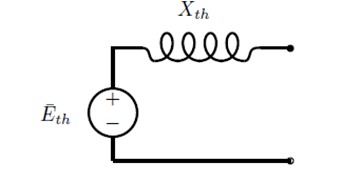
\includegraphics[width=0.5\linewidth]{Figure_Nordic/SMasACvoltageSource.png}
    \caption{Synchronous Machine Representation as AC Voltage source}
    \label{fig:AC}
\end{figure}
This is the first stage of test model benchmarking. The original Nordic System is used with its line and transformer parameters intact but with the synchronous machine (SM) replaced by AC voltage sources as shown in Fig. \ref{fig:AC}. This setup provides initial validation of the operating point for the load flow solution. The EMTP file in the shared folder is named \textbf{NordicACSource.ecf}.

\textbf{Equivalent SM representation}
\begin{itemize}
    \item Simple Representation of SM as a voltage source $E^"$ behind the sub transient reactance $X_d^{"}$- used in short circuit studies with steady-state phasor solutions, and reasonably accurate for transient studies for a few cycles of a transient disturbance. Switching surges also can be studied by this representation. Assumption: neglecting flux linkage changes in the field structure circuits.
    \item Simple Representation of SM as a voltage source $E^{'}$ behind the transient reactance $X_{d}^{'}$ for simplified stability studies. Assumption: neglecting flux linkage changes in the field structure circuits and damper winding currents have died out.
    \item Detailed Model Study- Used for sub-synchronous resonance studies as time span is too long to allow the use of a simplified model, for torsional dynamics of the shaft, for simulation of out-of-step synchronization.
\end{itemize}

\textbf{EMTP Specification for the test system:}
\begin{itemize}
    \item The first option \textit{i.e.} SM's simple representation as a Thevenin voltage source ($E_{th}$) behind the sub-transient reactance $X_{th}$ is considered as shown in fig. \ref{fig:AC}. The magnitude and angle of $E_{th}$ are the same as the buses' operating point in \cite{van2015test} for operating point A to be entered in \textit{kVRMSLL}, line to line RMS voltage and degree/radian respectively. 
    \item The value of $X_{th}$ is entered in real value so the per unit value needs to be multiplied by the base impedance.  
    \item With the generator bus a Load-Flow Bus is used that is available with constraint (bus) types are Slack-bus, PQ-control and PV-control, it considers the voltage and angle from the initial load flow data obtained from \cite{van2015test} and updates the source impedance as internal Thevenin impedance matrix of the source attached to the reference bus.
    \item All transformers must be of the Y-Y type since the phase shift is not considered in phasor-mode simulation. So, the connection of the transformer is set to star grounded type. The magnetizing branch model is excluded. Increasing the tap ratio increases the voltage on the secondary. 
    \item Line is chosen as a PI line 3-phase and the resistance and reactance are directly entered as ohm value that can be obtained from the transmission line data-sheet in \cite{van2015test}. While the susceptance value is given as $Y_c=j\omega C$, so B value is written (instead of B/2). 
    \item For shunt component RLC Load is chosen for 3-phase devices where voltage is entered as nominal voltage and reactive power with sign: Inductor +ve and Capacitor -ve. 
    \item For load: PQ load with load-flow (LF) is selected from the library which is used both as 1-phase and 3-phase. The entry for active and reactive power is to be done for a single phase. It participates in the load flow and all other solution options.
\end{itemize}

\textbf{Load Flow Results:} Using the \textit{Find Load Flow Solution} option in the EMTP Software and using the \textit{View Steady-State} the result is obtained both on SSPhasor in the EMTPWorks and also saved as \_lf.html format in the filename folder. The nominal voltage need to be specified in the properties for the bus as mentioned in Fig. \ref{fig:properties}. This is important as the nominal voltage is used in p.u. calculations for Steady-State (or Load-FLow) phasors. The electrical network equations are solved using complex phasors. The active (source) devices are only the Load-Flow devices (LF-devices). A load device is used to enter PQ load constraint equations. Only a single (fundamental) frequency solution is achievable in this version. The solution frequency is specified by ‘Default Power Frequency’ and used in passive network lumped model calculations. The EMTP Load-Flow solution can work with multiphase and unbalanced networks. The control system devices are disconnected and not solved. The load flow results in a comparison of the EMTP and STEPSS is provided in the table for the Generator, Load, and Shunt components in Table \ref{Generator}, \ref{Load} and \ref{Shunt} respectively.
In STEPSS the power flow iterations are stopped once all P and Q mismatches are less than 0.1 MW and 0.1 Mvar, respectively. 
Load flow matching ensures that the grid component parameters—such as transformer ratios, shunt branches, and line parameters—are correctly configured. Once confidence in network modeling is achieved, the next step is detailed synchronous machine design, which is discussed in the following section. 
\begin{figure}
    \centering
    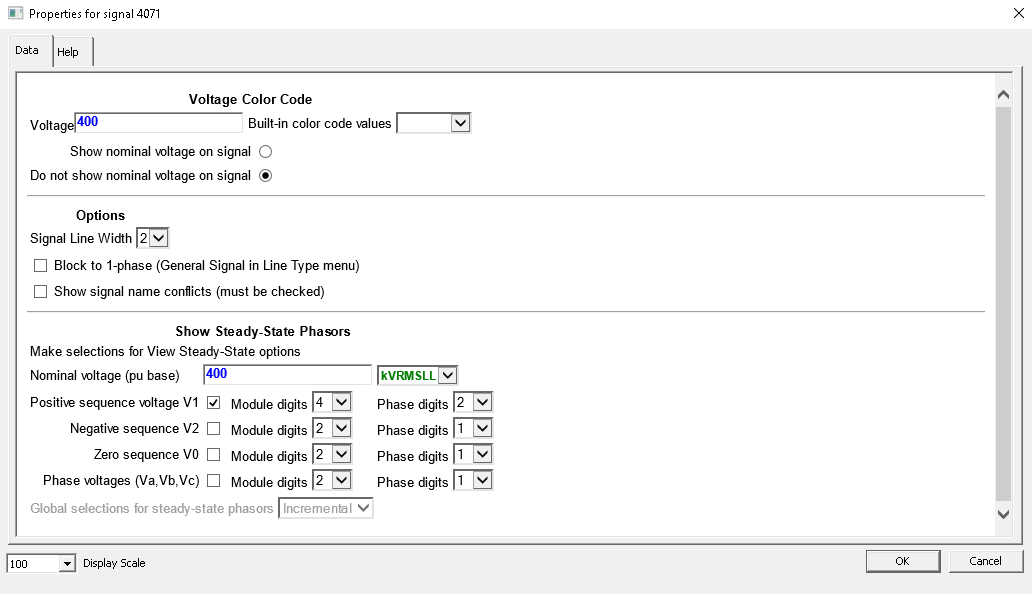
\includegraphics[width=0.8\linewidth]{Figure_Nordic/Properties.png}
    \caption{Properties of the bus, marking the base value}
    \label{fig:properties}
\end{figure}
\begin{table}
\centering
\caption{Comparison of Generator Bus Load Flow between EMTP and STEPSS}
\begin{tabular}{c| l l l c| l l l c| } 
 & &  & EMTP &  & &  & STEPSS &  \\ 
Generator & P  & Q & Vmag  & Vangle  & P & Q & Vmag & Vangle \\ 
& (MW) & (MVar) &  (p.u.) & (deg) & (MW) & (MVar) &  (p.u.) & (deg)\\
\hline
G20 & 2137.41 & 377.39 & 1.0185 & 0 & 2137.3 & 377.4 & 1.0185 & 0 \\ 
G1 & 600 & 58.34 & 1.0684 & 2.58 & 600 & 58.3 & 1.0684 & 2.59 \\ 
G2 & 300 & 17.24 & 1.0565 & 5.12 & 300 & 17.2 & 1.0565 & 5.12 \\ 
G3 & 550 & 20.92 & 1.0595 & 10.27 & 550 & 20.9 & 1.0595 & 10.28 \\ 
G4 & 400 & 30.39 & 1.0339 & 8.03 & 400 & 30.4 & 1.0339 & 8.03 \\ 
G5 & 200 & 60.09 & 1.0294 & -12.36 & 200 & 60.1 & 1.0294 & -12.36 \\ 
G6 & 360 & 138.57 & 1.0084 & -59.42 & 360 & 138.5 & 1.0084 & -59.4 \\ 
G7 & 180 & 60.42 & 1.0141 & -68.95 & 180 & 60.4 & 1.0141 & -68.95 \\ 
G8 & 750 & 232.59 & 1.0498 & -16.8 & 750 & 232.5 & 1.0498 & -16.8 \\ 
G9 & 668,5 & 201.28 & 0.9988 & -1.63 & 668,5 & 201.2 & 0.9988 & -1.63 \\ 
G10 & 600 & 255.71 & 1.0157 & 0.99 & 600 & 255.7 & 1.0157 & 0.99 \\ 
G11 & 250 & 60.73 & 1.0211 & -29.04 & 250 & 60.7 & 1.0211 & -29.04 \\ 
G12 & 310 & 98.34 & 1.02 & -31.88 & 310 & 98.3 & 1.02 & -31.88 \\ 
G13 & 0 & 50.12 & 1.017 & -54.3 & 0 & 50 & 1.017 & -54.29 \\ 
G14 & 630 & 295.86 & 1.0454 & -49.9 & 630 & 295.7 & 1.0454 & -49.89 \\ 
G15 & 1080 & 377.91 & 1.0455 & -52.19 & 1080 & 377.8 & 1.0455 & -52.18 \\ 
G16 & 600 & 222.63 & 1.0531 & -64.1 & 600 & 222.5 & 1.0531 & -64.09 \\ 
G17 & 530 & 48.73 & 1.0092 & -46.86 & 530 & 48.7 & 1.0092 & -46.85 \\ 
G18 & 1060 & 293.43 & 1.0307 & -43.32 & 1060 & 293.4 & 1.0307 & -43.32 \\ 
G19 & 300 & 121.24 & 1.03 & 0.03 & 300 & 121.2 & 1.03 & 0.03 \\ 

\end{tabular}
\label{Generator}
\end{table}

\begin{table}
\centering
\caption{Comparison of Load Bus Load Flow between EMTP and STEPSS}
\begin{tabular}{c| l l l c| l l l c| } 
 & &  & EMTP &  & &  & STEPSS &  \\ 
Load & P  & Q & Vmag  & Vangle  & P & Q & Vmag & Vangle \\ 
& (MW) & (MVar) &  (p.u.) & (deg) & (MW) & (MVar) &  (p.u.) & (deg)\\
\hline
L1 & 600 & 148.2 & 0.9988 & -84.7 & 600 & 148.2 & 0.9988 & -84.7 \\
L2 & 330 & 71 & 1.0012 & -70.48 & 330 & 71 & 1.0012 & -70.48 \\
L3 & 260 & 83.8 & 0.9975 & -79.96 & 260 & 83.8 & 0.9975 & -79.96 \\
L4 & 840 & 252 & 0.9997 & -70.66 & 840 & 252 & 0.9997 & -70.66 \\
L5 & 720 & 190.4 & 0.9961 & -74.58 & 720 & 190.4 & 0.9961 & -74.58 \\
L11 & 200 & 68.8 & 1.0026 & -9.45 & 200 & 68.8 & 1.0026 & -9.45 \\
L12 & 300 & 83.8 & 0.9975 & -5.93 & 300 & 83.8 & 0.9975 & -5.93 \\
L13 & 100 & 34.4 & 0.9957 & -1.58 & 100 & 34.4 & 0.9957 & -1.58 \\
L22 & 280 & 79.9 & 0.9953 & -21.89 & 280 & 79.9 & 0.9953 & -21.89 \\
L31 & 100 & 24.7 & 1.0042 & -39.46 & 100 & 24.7 & 1.0042 & -39.46 \\
L32 & 200 & 39.6 & 0.9978 & -26.77 & 200 & 39.6 & 0.9978 & -26.77 \\
L41 & 540 & 131.4 & 0.9968 & -57.14 & 540 & 131.4 & 0.9968 & -57.14 \\
L42 & 400 & 127.4 & 0.9953 & -60.21 & 400 & 127.4 & 0.9953 & -60.21 \\
L43 & 900 & 254.6 & 1.0013 & -66.32 & 900 & 254.6 & 1.0013 & -66.32 \\
L46 & 700 & 211.8 & 0.9991 & -66.93 & 700 & 211.8 & 0.9991 & -66.93 \\
L47 & 100 & 44 & 0.995 & -62.37 & 100 & 44 & 0.995 & -62.37 \\
L51 & 800 & 258.2 & 0.9978 & -73.83 & 800 & 258.2 & 0.9978 & -73.83 \\
L61 & 500 & 122.5 & 0.9949 & -60.78 & 500 & 122.5 & 0.9949 & -60.78 \\
L62 & 300 & 83.8 & 1.0002 & -57.17 & 300 & 83.8 & 1.0002 & -57.17 \\
L63 & 590 & 264.6 & 0.9992 & -53.48 & 590 & 264.6 & 0.9992 & -53.48 \\
L71 & 300 & 83.8 & 1.0028 & -7.8 & 300 & 83.8 & 1.0028 & -7.8 \\
L72 & 2000 & 396.1 & 0.9974 & -6.83 & 2000 & 396.1 & 0.9974 & -6.83 \\

\end{tabular}
\label{Load}
\end{table}


\begin{table}
\centering
\caption{Comparison of Shunt Bus Load Flow between EMTP and STEPSS}
\begin{tabular}{c|l l l l c|}    
 & \multicolumn{2}{l}{EMTP} & STEPSS \\
Shunt & \multicolumn{2}{l}{Q} & Q \\
Shunt & \multicolumn{2}{l}{(MVar)} & (MVar)) \\
\hline
1022 & \multicolumn{2}{l}{55.29} & 55,3 \\
1041 & \multicolumn{2}{l}{256,24} & 256,3 \\
1043 & \multicolumn{2}{l}{211,13} & 211,1 \\
1044 & \multicolumn{2}{l}{202,64} & 202,7 \\
1045 & \multicolumn{2}{l}{204,45} & 204,5 \\
4012 & \multicolumn{2}{l}{-104,77} & -104,8 \\
4041 & \multicolumn{2}{l}{220,75} & 220,8 \\
4043 & \multicolumn{2}{l}{215,06} & 215,1 \\
4046 & \multicolumn{2}{l}{107,27} & 107,3 \\
4051 & \multicolumn{2}{l}{113,62} & 113,6 \\
4071 & \multicolumn{2}{l}{-439,69} & -439,7 \\
\end{tabular}
\label{Shunt}
\end{table}

 \textbf{Steady-State solution: }
When the Simulation Options for the \textit{Steady State solution} are selected, starting from the Load-flow solution, the simulator generates the node voltage, transmitted power (1-phase), and generated power. It also calculates the power balance and generates an HTML file with the results. Few other details like the total number of network nodes including internal nodes: 582, The size of the main system of equations: 942. 
The other detail of the simulation time is mentioned in Table \ref{SSS1}. Total CPU time taken in EMTP is 15.367188 seconds while STEPSS uses parallel computing and simulation takes 1.1080 seconds as shon in Fig. \ref{fig:STEPSSDS}. 

\begin{table}
\centering
\caption{Steady State Simulation Timers}
\begin{tabular}{l| l} 
 CPU timers &  second\\
 \hline
 Prepare data&  0.00781\\
 Read data&  0\\
 Device initialization&  0\\
 Network Topology initialization&  0\\
 Steady-state solution&  0.12500\\
 Time-domain A matrix formulation&  0\\
 Time-domain B vector updating&  0\\
 Time-domain reformulations&  0\\
 Time-domain Ax=B solution&  2.46875\\
 Solution of control systems&  0.02344\\
 Time-domain history updating&  0\\
 Time-domain solution&  15.17188\\
 \hline
 Total&  15.367188\\

\end{tabular}
\label{SSS1}
\end{table}
\begin{figure}
    \centering
    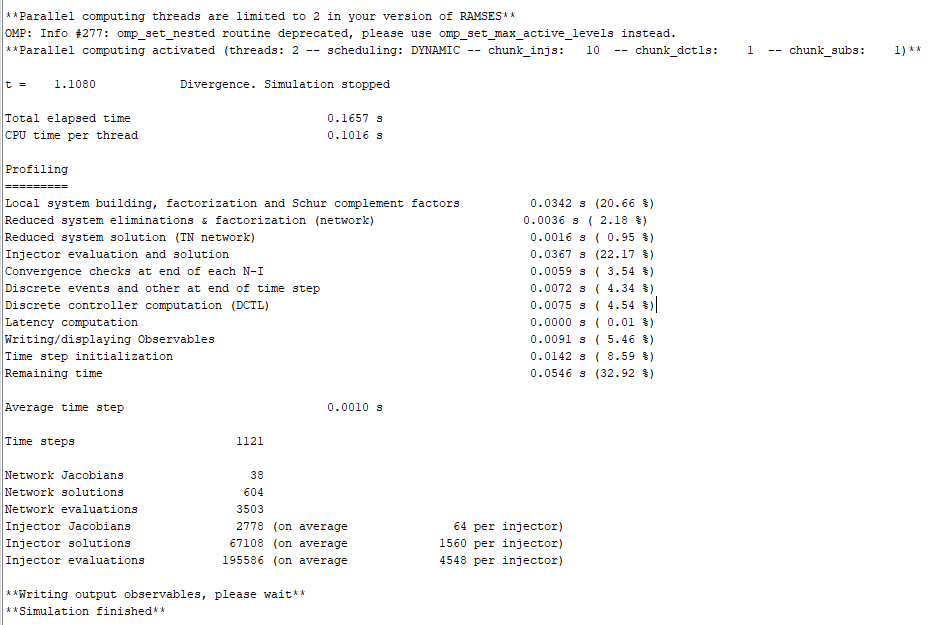
\includegraphics[width=1\linewidth]{Figure_Nordic/STEPSSDynamicSimulationDetail.png}
    \caption{STEPSS dynamic simulation details}
    \label{fig:STEPSSDS}
\end{figure}

\subsubsection{[II] Test system with Single Machine Infinite Bus}
%Synchronous machine EMTP modeling is detailed in this section.\\ 
\textbf{SM Modelling Convention in EMTP} 
\begin{itemize}
    \item Generator convention is used for all windings, each winding 'k' is described by:
    \begin{equation}
        v_k(t)=-R_ki_k(t) - \frac{d\lambda_k(t)}{dt}
    \end{equation}
    \item In steady state, the machine's internal emf (proportional to field current) is aligned along the q axis. quadrature axis lagging $90^o$ behind the direct axis in the machine phasor diagram is adopted in EMTP thus positive sign is used in the second row of transformation matrix. The transformation matrix of abc to dq0 frame is normalized and the power invariant in EMTP software inductance matrix in dq0 is always symmetric. The unnormalized convention uses a factor 2/3 corresponding to the d and q row and 1/3 corresponding to the 0 row.
    \item All reactances and time constants are unsaturated values because saturation is considered separately. Thus short-circuit time constants are preferred over open-circuit time constants where measurements are not influenced by saturation effects.
    \item The machine per unit values are on the machine-rated base value while the exciter and turbine have base values that are different from the machine base. The $I_{fd}^{rated}$ (pu)  values are in per unit on a base such that $i_{fd}$= 1 pu when the generator operates at no load with a 1 pu terminal voltage and without saturation (operation on the air gap line). Here it is to be marked that $i_{fd}$ real value is to be entered but the base value of the exciter is not mentioned in the document. So an industrial preferred value is randomly taken, for example, for a 500 MVA machine to generate 1 pu terminal voltage a value of 1000 A field current is required. 
    \item Saturation is modeled in all machines separately, which represents, relation giving the flux with respect to the currents is no longer linear; it is not represented by a single straight line (air gap line). It is difficult to model saturation very accurately. The data requirements are different while modeling in EMTP. Saturation characteristics are given by: $k=1 + m(V_{nl})^n$. 
    As per \cite{van2015test}, for armature voltage ($V_{nl}$) of 1 p.u., k=1.1, which yields, m=0.1, and excitation current needed is: $i_{1.0}$=(k*1.0*$i_o$). And for $V_{nl}$ =1.2 pu, k=1.3, which yields, n=6.0257 and excitation current needed: $i_{1.2}$ =(k*1.2*$i_o$) as shown in fig. \ref{fig:saturation}.
        \begin{figure}[H]
        \centering
        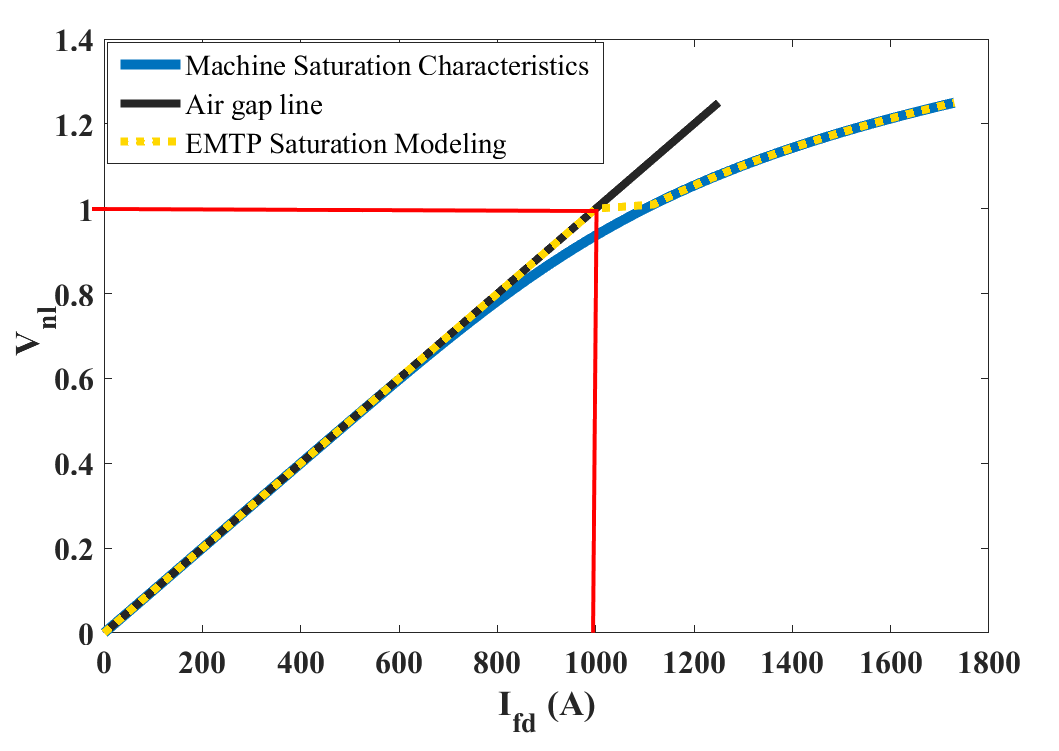
\includegraphics[width=0.7\linewidth]{Figure_Nordic/Saturation.png}
        \caption{Saturation Characteristics}
        \label{fig:saturation}
    \end{figure}
    \begin{figure}
    \centering
    \includegraphics[width=0.5\linewidth]{EMTPSat.png}
    \caption{EMTP tab for saturation data}
    \label{fig:EMTPSat}
    \end{figure}
   
    The incorporation of machine saturation is more detailed in EMTP, offering finer granularity in response characteristics. The saturation in the synchronous machine model follows a piecewise linear characteristic and always starts at $i_{fd}$ for 1 pu armature voltage without saturation (operation on the air gap line). The slope of each segment shall decrease with the increase of voltage. To have a good match with saturation characteristics multiple V,I points are calculated from the formula, and then a piecewise linear approximation between these points as shown in fig.\ref{fig:EMTPSat}. The difference in saturation characteristics in EMTP modeling is clearly illustrated in fig.\ref{fig:saturation}. The curve follows the airgap line up to 1 p.u. voltage and then, using a piecewise approximation, aligns with the machine's saturation characteristics.
As mentioned above, there are discrepancies in modeling saturation between EMTP and STEPSS. Since the project aims to clearly differentiate between EMT and RMS simulations, these discrepancies at the simulator level need to be minimized.

For modeling saturation, it is essential to know the field current value in amperes that produces a 1 pu armature voltage, without considering saturation ("on the air gap line"). However, this information is not available in the phasor model and data (in STEPSS), as the entire phasor model is in per unit. It is assumed that the correct field current base has been used in the field winding to derive the per-unit values of the machine parameters, but this base value is unknown. Therefore, we cannot retrieve the field current values in amperes from the document \cite{van2015test}. Nonetheless, values per unit are sufficient because the machine's behavior should not depend on the base value.

Since providing a field current value is mandatory in EMTP, we use a plausible dummy value, such as 1000 A (1 kA) for the 500-MVA machine g19. A detailed comparison is then presented between cases with and without saturation. The saturation in the synchronous machine in the EMTP model follows a piecewise linear characteristic. The slope of each segment shall decrease with the increase of voltage. To have a good match with STEPSS we calculate V, and I points from the formula and EMTP will apply a piecewise linear approximation between these points as shown in Fig.\ref{fig:EMTPSat}
    
    \item The excitation system and the turbine are modeled in their own per-unit systems. The parameters of the turbine are expressed in per unit on the turbine nominal power, $P_{nom}$ base (in MW). The synchronous machine refers to the machine's nominal apparent power $S_{nom}$ (in MVA). Both $P_{nom}$ and  $S_{nom}$  are specified for each machine. An example of generator 19 data is shown in Table \ref{tab:G19} \cite{van2015test}.
\begin{table}[H]
\centering
\caption{Nominal apparent power of Synchronous machine 19 and nominal active power of its turbine}
\begin{tabular}{|c|c|c|}
    \hline
    Generator & $S_{nom}$ & $P_{nom}$ \\
    \hline
    G19 & 500 & 475 \\
    \hline
\end{tabular}
\label{tab:G19}
\end{table}
However, in EMTP only the machine base ($S_{nom}$) is considered. So change of base is thus necessary to interface those models. In the case of Generator 19, the initial mechanical torque is Tm = 0.63158 p.u., on the turbine base, which is defined on $P_{nom}$ (which is 475 MW for G19) parameter of the machine. To convert from the machine base ($S_{nom}$ which is 500 MVA) to the turbine base, we use:
$p.u._{NEW}=p.u._{OLD}*\frac{Base_{OLD}}{Base_{NEW}}$.  
Multiplying by $S_{nom}/P_{nom}$ (=500/475=1.05263) to change the base to the turbine base. 
\end{itemize}
%Base Current:  $I_{base}=\frac{S_{nom}}{\sqrt{3} V_b}$


\textbf{Initialization:}
In EMTP certain blocks like the transfer function, integral, PI controller, and others, need to define the initial history of the output signal as it highly influences the initial dynamics.
The overall generator control is shown in fig. \ref{fig:GControl}. Output from the generator block, $E_{fss}$ is Steady-state field voltage (on d-axis) in p.u., $\upsilon$ is the magnitude of the generator terminal voltage, in p.u., $\omega$ is the angular velocity, $P_{mss}$ is total mechanical steady state power and $P_e$ is total electric power. $\upsilon_{fd}$ is the field voltage, per unit on a base such that $\upsilon_{fd}$  = 1 p.u. when the generator operates at no load with a 1 p.u. terminal voltage and without saturation (operation on the air gap line). $T_m$ is the total mechanical torque. $\upsilon_{pss}$ is the power system stabilizer signal in p.u.
\begin{figure}[H]
    \centering
    \includegraphics[width=0.5\linewidth]{Figure_Nordic/GeneratorControl.png}
    \caption{Generator Control}
    \label{fig:GControl}
\end{figure}

\textbf{Exciter, automatic voltage regulator and power system stabilizer model:}
A simple model of the first-order system with a time constant of 0.1s and a non-windup limit on field voltage is used to represent the exciter. The Automatic Voltage Regulator (AVR) includes a transient gain reduction. All generators except g13,g19, and g20 are equipped with the Power System Stabilizer (PSS) using rotor speed in p.u. as input. The PSS transfer functions provide damping for oscillation frequencies from 0.2 Hz to more than 1 Hz. The overexcitation limiter model is not considered in the study as the study is concerned with short-term voltage stability. Each generator uses the same model but has different parameterizations as mentioned in \cite{van2015test}. Fig.\ref{fig:exciter} shows the exciter, AVR model.  At the initial operating point, the field voltage is on the exciter base, which is indirectly defined by the base of the excitation system and machine ratio. In EMTP Exciter SEXS from the library is modified to model it near the one mentioned in fig. \ref{fig:exciter}. In EMTP the subcircuit can be masked to fill the data directly in the display property tab. Fig.\ref{fig:ExciterEMTP} shows the Exciter model and the pin description are: VREF-input reference voltage of the stator terminal voltage (p.u.), Efss-input steady-state field voltage at t = 0, for initialization (p.u.) obtained from the synchronous machine observe selections, VC-input terminal voltage of synchronous machine (p.u.) calculated from the observer selection d and q-axis voltage norm ($\sqrt{v_d^2+v_q^2}$), VS- input Power System Stabilizer (PSS) signal (p.u.) obtained from PSS block defined in fig.\ref{fig:PSSEMTP}. EFD is output of the exciter block that provide field voltage signal (p.u.) to the synchronous machine.  
\begin{figure}[H]
    \centering
    \includegraphics[width=0.7\linewidth]{Figure_Nordic/Exciter.png}
    \caption{Modified model of exciter for short-term voltage stability study}
    \label{fig:exciter}
\end{figure}
\begin{figure}
    \centering
    \includegraphics[width=1.0\linewidth]{Figure_Nordic/ExciterEMTP.png}
    \caption{EMTP model representing small test  system with two machines}
    \label{fig:ExciterEMTP}
\end{figure}
\begin{figure}
    \centering
    \includegraphics[width=1.0\linewidth]{Figure_Nordic/PSSEMTP.png}
    \caption{EMTP model representing power system stabilizer}
    \label{fig:PSSEMTP}
\end{figure}

To find the history parameters of the blocks in EMTP, equations are analyzed in Fig. \ref{fig:exciter}. The PSS term is removed in the case study for G13, G19, and G20. For initialization of the blocks, the system is assumed in a steady state: $\frac{d}{dt}$ term is zero.  The history can be derived from the following equations: 

$\upsilon_{fd}=(\upsilon_i-\upsilon_{fd})10.\frac{1}{s} \implies \frac{1}{10}\frac{d\upsilon_{fd}}{dt} = (\upsilon_i-\upsilon_{fd}) \implies \upsilon_i(0)=\upsilon_{fd}(0)  $

$ \upsilon_i = d\upsilon.\frac{G(1+s.T_a)}{(1+s.T_b)} \implies \upsilon_i +T_b\frac{d\upsilon_i}{dt} = Gd\upsilon + GT_a\frac{d\upsilon}{dt} \implies d\upsilon(0)=\upsilon_i(0)/G \implies d\upsilon$(0)=$\frac{v_{fd}(0)}{G}$

$d\upsilon=V^o\ -\upsilon\ +\upsilon_{pss} \implies V^o=\upsilon(0)+d\upsilon(0)$.

 Thus the history of the output signal for the blocks is summarized as:
 \begin{table}[H]
\centering
\caption{History Block}
\begin{tabular}{|c|c|}
    \hline
For Exciter [1/s] block: & $V_{fd}$ (0)= $E_{fss}(0) $ \\
\hline
For AVR $\frac{G(1+s.T_a )}{(1+s.T_b)}$ block: &($V_{fd}$ (0))/G=$E_{fss}(0)/G$\\
\hline
Reference Voltage &$V^o=\upsilon(0)+V_{fd}/G$ \\
    \hline
\end{tabular}
\label{tab:HistoryExciter}
\end{table}

\textbf{Governor-Turbine Model}
As shown in fig \ref{fig:Speed} and \ref{fig:turbine} and described in \cite{van2015test}, North, and Equivalent have hydro generation and are equipped with speed governor control. Central and South have thermal power generation but lack speed control. Table \ref{tab:HistoryGovTurbine} details the history block input in various block in EMTP as shown in Fig. \ref{fig:GovernorEMTP}. The governor turbine- HYGOVR model is considered from the library which is modified to obtain a similar model as given in the report. Pin description of the model: Pref-input power reference from load controller, Pm-ic- input steady-state mechanical power at t =0 (p.u.) obtained from the observe $P_{mss}$ signal of the SM, w- input mechanical speed (p.u.) obtained from the machine model angular velocity (omega-i), Pe- input electrical power (p.u.). Output pins are g-pos- gate position (p.u.), Pm- turbine mechanical power (p.u.). The detail of pin selection in the synchronous machine model is mentioned in Fig. \ref{fig:EMTPSMtab} and \ref{fig:EMTPSMtab2} for the selection of electrical and mechanical signals from the SM model. 

 \begin{table}[H]
\centering
\caption{History Block}
\begin{tabular}{|c|c|}
    \hline
For Governor PI [1/s] block: & $z(0)$ = $P_{mss}(0) $ \\
    \hline
For Governor  [1/1+s2] block: & =$P_e(0)$  \\
\hline
For Sevomotor  [1/s] block: & $z(0)$ = $P_{mss}(0) $ \\
\hline
Reference Power &$P^o$ =$P_e(0)$ \\
\hline
For Turbine  [1/s] block: & $z(0)$ = $P_{mss}(0) $ \\
    \hline
\end{tabular}
\label{tab:HistoryGovTurbine}
\end{table}

\begin{figure}
    \centering
    \includegraphics[width=0.7\linewidth]{Figure_Nordic/SpeedGovernor.png}
    \caption{Model of Speed Governor}
    \label{fig:Speed}
\end{figure}

\begin{figure}
    \centering
    \includegraphics[width=0.7\linewidth]{Figure_Nordic/HydroTurbine.png}
    \caption{Hydro Turbine}
    \label{fig:turbine}
\end{figure}
\begin{figure}
    \centering
    \includegraphics[width=1.0\linewidth]{Figure_Nordic/GovernorTurbineEMTP.png}
    \caption{EMTP model representing governor turbine}
    \label{fig:GovernorEMTP}
\end{figure}

\begin{figure}
    \centering
    \includegraphics[width=0.5\linewidth]{Figure_Nordic/EMTPSM.png}
    \caption{Property tab of synchronous machine model of EMTP, if the Observe option is selected, the corresponding signal becomes automatically available in the observe signal bundle of the machine. If the Scope option is selected, the selected variable will become available under machine scopes.
 }
    \label{fig:EMTPSMtab}
\end{figure}
\begin{figure}
    \centering
    \includegraphics[width=0.5\linewidth]{Figure_Nordic/EMTPMechanicalData.png}
    \caption{Mechanical data tab of the  synchronous machine model of EMTP,}
    \label{fig:EMTPSMtab2}
\end{figure}
Fig. \ref{fig:G9G20} shows the EMTP model of SMIB. The SM G20 block is modeled as infine voltage source as shown in fig. \ref{fig:ACSM}.  While the SM G9 block is a detail synchronous generator model as shown in fig. \ref{fig:SGDetail} considering the exciter, PSS, and governor-turbine model input to the SM model. The SMIB test is done for all types of SM used in the system as discussed below: 
\begin{figure}
    \centering
    \includegraphics[width=0.8\linewidth]{Figure_Nordic/Results/G9G20/EMTPG9G20Model.png}
    \caption{SMIB Model of G9 and G20 with scenario-Fault Line Break}
    \label{fig:G9G20}
\end{figure}
\begin{figure}
    \centering
    \includegraphics[width=0.8\linewidth]{Figure_Nordic/SMasACVoltageSource.JPG}
    \caption{EMTP model representing synchronous machine as AC Voltage source}
    \label{fig:ACSM}
\end{figure}

\begin{figure}
    \centering
    \includegraphics[width=0.8\linewidth]{Figure_Nordic/SynchronousGeneratorEMTP.png}
    \caption{EMTP model representing detail synchronous machine with exciter, AVR, PSS, turbine and governor}
    \label{fig:SGDetail}
\end{figure}

\textbf{II.A. Generator with Governor-Turbine and Exciter without PSS:} Example case of single Machine (G19) Infinite Bus -SMIBG19. G19 is modeled as a detailed synchronous generator.
[Note: G19 does not have a PSS]. G20 is a Thévenin equivalent (SCC = 30,000 MVA) imposing a constant frequency, the speed governor model of g19 cannot be tested either. Fig.\ref{fig:SMIBG19} highlights the response of active power (P (MW)), rotor speed ($\omega_r$(p.u.)), field voltage ($V_f$(p.u.)), and terminal voltage (G19-$V_t$(p.u.)) of generator 19 for all scenarios:  i) Set Point change ii) fault at bus 4072 and iii) fault cleared by line break scenario with machine modelled without and with saturation. From this test case response verification of the exciter model can be claimed. 

\begin{figure}[htbp]
  \centering
  \subfloat[SMIB of SM19 modeled without saturation- Scenario:Increase in Voltage set point change by 0.05p.u.]{
    \includegraphics[width=0.46\textwidth]{Figure_Nordic/Results/SMIBG19/G19UnSatSetPointChange.pdf}
    \label{fig:G19UnSatSPC}
  }
  \hfill
  \subfloat[SMIB of SM19 modeled with saturation- Scenario:Increase in Voltage set point change by 0.05p.u.]{
    \includegraphics[width=0.46\textwidth]{Figure_Nordic/Results/SMIBG19/G19SatSetPointChange.pdf}
    \label{fig:G19SatSPC}
  }
  \\
    \subfloat[SMIB of SM19 modeled without saturation- Scenario:Fault at Bus 4072 cleared at 1.1 second]{
    \includegraphics[width=0.46\textwidth]{Figure_Nordic/Results/SMIBG19/G19UnSatFault.pdf}
  }
  \hfill
  \subfloat[SMIB of SM19 modeled with saturation- Scenario:Fault at Bus 4072 cleared at 1.1 second]{
    \includegraphics[width=0.46\textwidth]{Figure_Nordic/Results/SMIBG19/G19SatFault.pdf}
    \label{fig:G19SatFault}
  }
  \\
      \subfloat[SMIB of SM19 modeled without saturation- Scenario:Fault at Bus 4072 cleared by line break]{
    \includegraphics[width=0.46\textwidth]{Figure_Nordic/Results/SMIBG19/G19UnSatFaultLineBreak.pdf}
    \label{fig:G19UnSatFLB}
  }
  \hfill
  \subfloat[SMIB of SM19 modeled with saturation- Scenario:Fault at Bus 4072 cleared by line break]{
    \includegraphics[width=0.46\textwidth]{Figure_Nordic/Results/SMIBG19/G19SatFaultLineBreak.pdf}
    \label{fig:G19SatFLB}
  }
  \caption{SMIB of SM19 modeled without and with saturation- with different case Scenarios}
  \label{fig:SMIBG19}
\end{figure}

\begin{figure}[htbp]
  \centering
  \subfloat[SMIB of SM9 modeled without saturation- Scenario:Increase in Voltage set point change by 0.05p.u.]{
    \includegraphics[width=0.46\textwidth]{Figure_Nordic/Results/SMIBG9/G9UnSatSetPointChange.pdf}
    \label{fig:G9UnSatSPC}
  }
  \hfill
  \subfloat[SMIB of SM9 modeled with saturation- Scenario:Increase in Voltage set point change by 0.05p.u.]{
    \includegraphics[width=0.46\textwidth]{Figure_Nordic/Results/SMIBG9/G9SatSetPointChange.pdf}
    \label{fig:G9SatSPC}
  }
  \\
    \subfloat[SMIB of SM9 modeled without saturation- Scenario:Fault at Bus 4072 cleared at 1.1 second]{
    \includegraphics[width=0.46\textwidth]{Figure_Nordic/Results/SMIBG9/G9UnSatFault.pdf}
    \label{fig:G9UnSatFault}
  }
  \hfill
  \subfloat[SMIB of SM9 modeled with saturation- Scenario: Fault at Bus 4072 cleared at 1.1 second]{
    \includegraphics[width=0.46\textwidth]{Figure_Nordic/Results/SMIBG9/G9SatFault.pdf}
    \label{fig:G9SatFault}
  }
  \\
      \subfloat[SMIB of SM9 modeled without saturation- Scenario:Fault at Bus 4072 cleared by line break]{
    \includegraphics[width=0.46\textwidth]{Figure_Nordic/Results/SMIBG9/G9UnSatFaultLineBreak.pdf}
    \label{fig:G9UnSatFLB}
  }
  \hfill
  \subfloat[SMIB of SM9 modeled with saturation- Scenario:Fault at Bus 4072 cleared by line break]{
    \includegraphics[width=0.46\textwidth]{Figure_Nordic/Results/SMIBG9/G9SatFaultLineBreak.pdf}
    \label{fig:G9SatFLB}
  }
  \caption{SMIB of SM9 modeled without and with saturation- with different case Scenarios}
  \label{fig:SMIBG9}
\end{figure}

\begin{figure}
    \centering
    \includegraphics[width=1.0\linewidth]{Figure_Nordic/Results/SMIBG9/EMTPG9RUnSatandBSatFault.txt.png}
    \caption{SMIBG9 Fault Line Break Without and With Saturation Comparison of EMTP Model}
    \label{fig:SMIB9Comp}
\end{figure}

\textbf{II.B.Generator with Governor Turbine and Exciter with PSS:}Example case Single Machine (G9) Infinite Bus -SMIBG9. G9 is modeled as a detailed synchronous generator. [Note PSS is present]. G20 is a Thévenin equivalent (SCC = 30,000 MVA) imposing a constant frequency, the speed governor model of g9 cannot be tested either.
Fig.\ref{fig:SMIBG9} highlights the response of active power (P (MW)), rotor speed ($\omega_r$(p.u.)), field voltage ($V_f$(p.u.)), and terminal voltage (G19-$V_t$(p.u.)) of generator 19 for all scenarios as mentioned above. From this test case response verification of the exciter model with PSS can be claimed.  
Fig. \ref{fig:SMIB9Comp} shows EMTP simulation results for the system behavior with (blue solid line) and without (red solid line) saturation under a fault followed by a line break scenario. The active power and rotor speed responses of the G9-SM remain consistent in both cases, while there is a slight difference in the field voltage and terminal voltage with and without saturation, as expected. Given the very similar responses for set-point changes, so the study will now focus on the fault case with a fault followed by a line break. 

\textbf{II.C. Synchronous Condenser}
\begin{figure}
    \centering
    \includegraphics[width=0.9\linewidth]{Figure_Nordic/Results/SMIB13/G13SatFaultLineBreak.pdf}
    \caption{SMIBG13 Fault Line Break Without Saturation}
    \label{fig:SMIB13}
\end{figure}
Fig. \ref{fig:SMIB13} is the test case for the synchronous condenser with a solid black line that shows STEPSS response and dotted red line EMTP response of active power (P), rotor speed ($\omega_r$), field voltage ($V_f$), terminal voltage at bus G13 ($G13-V_t$) and reactive power (Q(MVar)). The reactive power settles at the initial value Q=   54.8 MVar.

\begin{figure}
    \centering
    \includegraphics[width=0.9\linewidth]{Figure_Nordic/Results/EMTPG16G20.png}
    \caption{Comparison between SM20 modeled as AC voltage source and as detailed SM}
    \label{fig:SMIB16Comp}
\end{figure}
\subsubsection{[III] Small test system with two detailed generators}
In the presence of a strong AC voltage source, the response becomes dominated by it. The difference in response can be seen in fig. \ref{fig:SMIB16Comp} with G20 as AC voltage source (solid red line) and G20 as detailed SM (solid blue line) in a small test system has been modeled the same as fig. \ref{fig:G9G20} with G16 as a detailed synchronous machine. Fig. \ref{fig:SMIB16Comp} shows the response with scenario fault followed by line break of rotor speed (Omega),active power (Pe), field voltage (Vf), and terminal voltage (Vt) of the G16 generator. AC voltage source dominates the governor action of the detailed model. So in a small test system the same as fig. \ref{fig:G9G20} with both G9 and G20 as a detailed synchronous machine is modeled and the response can be seen in fig. \ref{fig:G9G20_result}. The response of the observable of the torque controller in fig. \ref{fig:G9G20Torque}. The z and q variables of STEPSS and EMTP are shifted due to different base power they consider. EMTP consider the $S_{nom}$ as the base while STEPSS takes $P_{nom}$ as the base value for the hydro-turbine and governor model. 
\begin{figure}[htbp]
  \centering
  \subfloat[Active power, rotor speed and voltage of generator terminal response of generator 9 and 20 with scenario-Fault Line Break]{
    \includegraphics[width=0.8\textwidth]{Figure_Nordic/Results/G9G20/G9G20.png}
    \label{fig:G9G20_result}
  }
  \hfill
  \subfloat[Active power, rotor speed and voltage of generator terminal zoomed response of generator 9 and 20 with scenario-Fault Line Break]{
    \includegraphics[width=0.8\textwidth]{Figure_Nordic/Results/G9G20/G9G20Zoomed.png}
    \label{fig:G9G20_result_zoomed}
  }
  \end{figure}
\begin{figure}
    \centering
    \includegraphics[width=1.0\linewidth]{Figure_Nordic/L71C150.png}
    \caption{Comparing the governor response for 50\% load decrease at bus 71 on a small system having G9 and G20 detailed models.}
    \label{fig:G9G20Torque}
\end{figure}
\subsubsection{[IV] Standard Nordic Test System}
The final stage of test model benchmarking involves validating the Nordic system with a detailed machine model, following the validation of the network and machine model. The first validation with respect to STEPSS is to check the initial values of the field voltages (vf) and the mechanical torques (Tm) of synchronous machines.

Table \ref{tab:Vf} gives the detail of steady-State solution field voltages (denoted by "vf" in STEPSS) of all machines without and with saturation when compared in STEPSS and EMTP. 

\begin{table}[H]
\centering
\caption{steady-State solution field voltages of all machines without and with saturation when compared in STEPSS and EMTP.}
\begin{tabular}{l|l l| l l}  

Generator & Unsaturated & Vf & Saturated & Vf \\
 & STEPSS & EMTP & STEPSS & EMTP \\
\hline
G1 & 1.3576 &  1.35754 & 1.5161 & 1.51558\\
G2 & 1.1915  & 1.19136 & 1.3365 & 1.33618\\
G3 & 1.3363  &  1.33619 & 1.4777 & 1.47753\\
G4 & 1.2780  &  1.27783 & 1.4018  & 1.40130\\
G5 & 1.5249 & 1.52485 & 1.6707 &  1.67058\\
G6 & 2.6385 & 2.63864 & 2.7607 &  2.76064\\
G7 & 2.5674 & 2.56780 & 2.6861 & 2.68633 \\
G8 & 1.6044 & 1.60430 & 1.7754 & 1.77486\\
G9 & 1.4087 & 1.4085 & 1.5243 & 1.52399\\
G10 & 1.5697 & 1.56965 & 1.7161 & 1.71593\\
G11 & 1.5081 & 1.50819 &1.6398 & 1.63944\\
G12 & 1.6106 &  1.61065 &1.7528 & 1.75286\\
G13 & 1.2712 &  1.27150 &  1.4043 & 1.40412\\
G14 & 2.7063 &  2.70658& 2.8775 &  2.87754\\
G15 & 2.5491 &  2.54924 & 2.6973  & 2.69688\\
G16 & 2.4799 & 2.48004  & 2.6378  & 2.63734\\
G17 & 2.2600 &  2.26006 & 2.3390  & 2.33890\\
G18 & 2.4412 &  2.44119 & 2.5630  & 2.56284\\
G19 & 1.4268 &  1.42684 & 1.5769 & 1.57670\\
G20 & 1.2102 &  1.21023 & 1.3293 &  1.32900\\
\end{tabular}
\label{tab:Vf}
\end{table}

\begin{figure}[htbp]
  \centering
  \subfloat[Active power of Generator {6,7,17 and 20}- Nordic system modeled without saturation]{
    \includegraphics[width=0.46\textwidth]{Figure_Nordic/Results/NordicFull/Without_Saturation/PeUnSatFault.pdf}
  }
  \hfill
  \subfloat[Active power of Generator {6,7,17 and 20}- Nordic system modeled with saturation]{
    \includegraphics[width=0.46\textwidth]{Figure_Nordic/Results/NordicFull/With_Saturation/PeSatFault.pdf}
  }
  \\
    \subfloat[Rotor speed of Generator {6,7,17 and 20}- Nordic system modeled without saturation]{
    \includegraphics[width=0.46\textwidth]{Figure_Nordic/Results/NordicFull/Without_Saturation/wrUnSatFault.pdf}
  }
  \hfill
  \subfloat[Rotor speed of Generator {6,7,17 and 20}- Nordic system modeled with saturation]{
    \includegraphics[width=0.46\textwidth]{Figure_Nordic/Results/NordicFull/With_Saturation/wrSatFault.pdf}
    %\label{fig:G9SatFault}
  }
\\
      \subfloat[Voltage terminal of Generator {6,7,10 and 17} and Bus {1041,1042,4012,4062}- Nordic system modeled without saturation]{
    \includegraphics[width=0.46\textwidth]{Figure_Nordic/Results/NordicFull/Without_Saturation/VtUnSatFault.pdf}
  }
  \hfill
  \subfloat[Voltage terminal of Generator {6,7,10 and 17} and Bus {1041,1042,4012,4062}- Nordic system modeled with saturation]{
    \includegraphics[width=0.46\textwidth]{Figure_Nordic/Results/NordicFull/With_Saturation/VtSatFault.pdf}
  }
 \caption{Active power, rotor speed and terminal voltage response of Nordic system modeled without and with saturation- Scenario: Fault at Bus 4032}
  \label{fig:NordicFullFault}
\end{figure}

\begin{figure}[htbp]
  \centering
  \subfloat[Active power of Generator {6,7,17 and 20}- Nordic system modeled without saturation]{
    \includegraphics[width=0.46\textwidth]{Figure_Nordic/Results/NordicFull/Without_Saturation/PeUnSatFaultLineBreak.pdf}
  }
  \hfill
  \subfloat[Active power of Generator {6,7,17 and 20}- Nordic system modeled with saturation]{
    \includegraphics[width=0.46\textwidth]{Figure_Nordic/Results/NordicFull/With_Saturation/PeSatFaultLineBreak.pdf}
  }
  \\
    \subfloat[Rotor speed of Generator {6,7,17 and 20}- Nordic system modeled without saturation]{
    \includegraphics[width=0.46\textwidth]{Figure_Nordic/Results/NordicFull/Without_Saturation/wrUnSatFaultLineBreak.pdf}
  }
  \hfill
  \subfloat[Rotor speed of Generator {6,7,17 and 20}- Nordic system modeled with saturation]{
    \includegraphics[width=0.46\textwidth]{Figure_Nordic/Results/NordicFull/With_Saturation/wrSatFaultLineBreak.pdf}
    %\label{fig:G9SatFault}
  }
\\
      \subfloat[Voltage terminal of Generator {6,7,10 and 17} and Bus {1041,1042,4012,4062}- Nordic system modeled without saturation]{
    \includegraphics[width=0.46\textwidth]{Figure_Nordic/Results/NordicFull/Without_Saturation/VtUnSatFaultLineBreak.pdf}
  }
  \hfill
  \subfloat[Voltage terminal of Generator {6,7,10 and 17} and Bus {1041,1042,4012,4062}- Nordic system modeled with saturation]{
    \includegraphics[width=0.46\textwidth]{Figure_Nordic/Results/NordicFull/With_Saturation/VtSatFaultLineBreak.pdf}
  }
 \caption{Active power, rotor speed and terminal voltage response of Nordic system modeled without and with saturation- Scenario: Fault at Bus 4032 cleared by opening line}
  \label{fig:NordicFullFaultLB}
\end{figure}

\begin{figure}[htbp]
  \centering
  \subfloat[Field Voltage for Generators in Full Nordic System without saturation: Scenario Fault at Bus 4032]{
    \includegraphics[width=0.46\textwidth]{Figure_Nordic/Results/NordicFull/Without_Saturation/VfUnSatFault.pdf}
  }
  \hfill
    \subfloat[Field Voltage for Generators in Full Nordic System with saturation: Scenario Fault at Bus 4032]{
    \includegraphics[width=0.46\textwidth]{Figure_Nordic/Results/NordicFull/With_Saturation/VfSatFault.pdf}
 }
  \\
    \subfloat[Field Voltage for Generators in Full Nordic System without saturation: Scenario Fault at Bus 4032 cleared by line break]{
    \includegraphics[width=0.46\textwidth]{Figure_Nordic/Results/NordicFull/Without_Saturation/VfUnSatFaultLineBreak.pdf}
  }
  \hfill
    \subfloat[Field Voltage for Generators in Full Nordic System with saturation: Scenario Fault at Bus 4032 cleared by line break]{
    \includegraphics[width=0.46\textwidth]{Figure_Nordic/Results/NordicFull/With_Saturation/VfSatFaultLineBreak.pdf}
 }
 \caption{Field Voltage response of Nordic system modeled without and with saturation- Scenario: Fault at Bus 4032 and Fault at Bus 4032 cleared by line break}
  \label{fig:NordicVf}
\end{figure}

\textbf{Nordic test system: dynamic responses to contingencies}
In the power flow case loads are constant P and Q power. In the dynamic simulation, P with alpha=1 (constant current)  and Q with Beta=2 (constant impedance). The fault case and its scenario of fault at bus 4032 and fault at bus 4032 followed by line break of 4032 and 4044 the response is examined over the first 15 seconds. Active power and rotor speed of G6, G7, G17, and G20, and terminal voltage at bus G6, G10, 1041, and 1012 response of the Nordic system modeled without and with saturation with the scenario of fault at Bus 4032 in fig. \ref{fig:NordicFullFault} and scenario of fault at Bus 4032 cleared by opening line 4032 and 4044 in fig. \ref{fig:NordicFullFaultLB}. The EMTP response curve damps out the oscillation faster in comparison to the STEPSS curves. This leads the system to be more stable in EMTP. Fig. \ref{fig:NordicVf} provides the response of field voltage of generators G6-9, G11-12, G14-16, G18, and G20 for the above scenarios. 

\textbf{Effect of different time-step}\\
\textbf{EMTP}
Additionally, an important consideration when dealing with different solvers and simulators need to be considered: as a rule of thumb, if the oscillations have a period linked to the time step size (for instance divided by 2 if the step size is divided by 2) it might be a numerical artifact due to the integration method. On the other hand, there are some fast dynamics in the model, which can be unveiled when the step size is decreased. Stiffly stable numerical integration methods (such as backward Euler or Backward differentiation formula of order 2 like in STEPSS) tend to "erase" the fast dynamics when the step size is increased. They act as filters. For checking the step size is divided by 2 and repeat the integration. One can trust the numerical scheme if the results are very close to each other (i.e., not significantly different from a practical viewpoint). Fig. \ref{fig:50100microsec} and \ref{fig:2550microsec}, show the EMTP result when simulated at time-step 25, 50, and 100 microseconds. It can be seen that 25 microseconds and 50 microseconds have similar responses thus can trust the numerical scheme for 50 microseconds.  

\textbf{STEPSS}
In STEPSS: PLOT STEP is 0.001, i.e.
you ask STEPSS not to display a point in time that differs from the previous one by less than (or just) 0.001 second. However, if STEPSS is making time steps of - say - 0.005 s, it will not display successive points in time that differ by less than 0.005 s, except when solving discontinuities or when meeting convergence problems, in which case, the minimum time step will be used. In other words, STEPSS does not interpolate in between its time steps. The following difference in setting time -step need to be considered for STEPSS mode:

1. For the NORDIC test system with machines only :

In the disturbance file, the time step is set to 0.005 s (1/4 of a period at 50 Hz) and the minimum time step to 0.001 s.  Thus the syntax is :
  
  0.000 CONTINUE SOLVER BD 0.005 0.001 0.00 ABL

In the settings file, set the min plot step to 0.0005 s. Hence, all points in time will be displayed (since 0.0005 $<$ 0.001) The syntax is :

PLOT STEP  0.0005    ;

2. For the NORDIC test system with some VSCs and the 4-VSC test system: The time step needs to be reduced due to the presence of the VSCs. The following is used :

0.000 CONTINUE SOLVER BD 0.001 0.0005 0.00 ABL

PLOT STEP  0.0001 s  ;

\begin{figure}
    \centering
    \includegraphics[width=0.9\linewidth]{Figure_Nordic/Results/G16Outage/50-100us.png}
    \caption{Simulation with 50 and 100 microsecond microsecond time step}
    \label{fig:50100microsec}
\end{figure}
\begin{figure}
    \centering
    \includegraphics[width=0.9\linewidth]{Figure_Nordic/Results/G16Outage/25_50us.png}
    \caption{Simulation with 25 and 50 microsecond time step}
    \label{fig:2550microsec}
\end{figure}
\subsection{Implementation choice-Nordic system with VSCs}
In the Nordic system, 5 generators are replaced by VSCs with the same nominal power. Those generators had a large reactive power response to the disturbance (field currents limited by overexcitation limiters).  Loads are turned to constant current modified as decreasing the exponent $\beta$  from 2 to 1 and $\alpha$= 1 remains unchanged. The study is done for short-term dynamics thus focus on first 15 s after disturbance. Hence, the overexcitation limiters need not be modeled. Neither the transformer load tap changers. Further there is no overload capacity of VSCs (maximum current = nominal current) while the overexcitation limiters allow for a 5\% overload wrt the generator capability curves. Limitation of VSC current is “immediate” (no intentional delay), so the impact on grid voltage control is expected to be faster

The following case scenario is modeled with different generation mixes to study the effect of the Nordic system in the presence of VSCs.

•Case1: Nordic Test cases: Infinite Bus with VSC as SG:-SG7, SG12, SG11, SG14 ad SG6\\
•Case2: Nordic System with SG \{7,12,11,14,6\} replaced with VSCs\\

The step-up transformer connected to the generator in the Nordic system serves as the connecting transformer. Figure \ref{fig:SMVSC} illustrates the VSC connection to the Nordic system, where the PCC side is connected to the bus for the step-up transformer. Table \ref{tab:SMVSC} provides the initial operating points of the synchronous machines (SM) that the VSCs replace. The controlling parameters for the corresponding PCC are detailed in Table \ref{tab:SMPCC}.
\begin{table}[H]
\centering
\begin{tabular}{|l |l |l|}
\hline
Replaced SM & S\_nom (MVA) & Active Power P (MW) \\
\hline
SG7 (VSCg7) & 200 & 180 \\
SG12 (VSCg12) & 350 & 310 \\
SG11 (VSCg11) & 300 & 250 \\
SG14 (VSCg14) & 700 & 630 \\
SG6 (VSCg6) & 400 & 360 \\
\hline
\end{tabular}
\end{table}

\begin{figure}
    \centering
    \includegraphics[width=0.7\linewidth]{Figure_Nordic/SMIB.png}
    \caption{Test System 1-VSC}
    \label{fig:SMVSC}
\end{figure}

\begin{table}[H]
\centering
\caption{Details of the generator terminal where the synchronous generator is being replaced by VSCs.}
\begin{tabular}{|l |l| l| l| l|}
\hline
\textbf{Generator} & \textbf{Base Voltage} & \textbf{Generated Power} & \textbf{Initial Voltage}& \textbf{Initial Voltage} \\
\textbf{Name} & \textbf{(KV)} & \textbf{(MW+jMVar)} & \textbf{magnitude(p.u.)} & \textbf{Angle (degree)} \\
\hline
SG7 & 15.0 & 180+j60.4 & 1.0141 & -68.95 \\
SG12 & 15.0 & 310+j98.3 & 1.0200 & -31,88 \\
SG11 & 15.0 & 250+j60.7 & 1.0211 & -29,04 \\
SG14 & 15.0 & 630+j295.9 & 1.0454 & -49,90 \\
SG6  & 15.0 & 360+j138.6 & 1.0084 &-59,42 \\
\hline
\end{tabular}
\label{tab:SMVSC}
\end{table}


\begin{table}[H]
\centering
\caption{Details of the PCC where the synchronous generator is being replaced by VSCs.}
\begin{tabular}{|l |l| l| l| l|}
\hline
\textbf{PCC for} & \textbf{Base Voltage} & \textbf{Generated Power} & \textbf{Initial Voltage}& \textbf{Initial Voltage} \\
\textbf{SM} & \textbf{(KV)} & \textbf{(MW+jMVar)} & \textbf{magnitude(p.u.)} & \textbf{angle(degree)} \\
\hline
1043 (VSCg7) & 130 & 180+j34.133 & 1.0274 & -76.77 \\
4031 (VSCg12) & 400 & 310+j54.777 & 1.0367 & -39.46 \\
4021 (VSCg11) & 400 & 250+j28.992 & 1.0488 & -36.08 \\
4042 (VSCg14) & 400 & 630+j200.88 & 1,0428 & -57.37 \\
1042 (VSCg6) & 130 & 360+j83.6985 & 1.0145 & -67.38 \\
\hline
\end{tabular}
\label{tab:SMPCC}
\end{table}

Fig. \ref{fig:VSCsPQ}, details the active and reactive power generated by the VSCs when connected to the Nordic System at bus -1042, 1043, 4021, 4031, and 4042. Initially, there is a small mismatch, which has been minimized by incorporating a script for load flow calculation. The modeling of the VSCs and the initialization process are described in Chapter 1. It is important to note that a significant mismatch due to initialization can cause instability in synchronous generators. Therefore, minimizing the initial power mismatch is crucial, especially in a network dominated by synchronous machines.

\begin{figure}
    \centering
    \includegraphics[width=1\linewidth]{Figure_Nordic/NordicVSC.png}
    \caption{Active and reactive power  at bus 1042, 1043, 4021, 4031, and 4042 when SM {G6, G7, G11, G12, G14} replaced by VSCs}
    \label{fig:VSCsPQ}
\end{figure}
\section{Example Study}
\subsection{Comparison of loss of active power in the Nordic System}
In the Nordic system with all SM, when there is fault and fault followed by a line break, the STEPSS and EMTP show a very similar characteristics as can be seen in Fig. \ref{fig:NordicFullFault} and \ref{fig:NordicFullFaultLB}. But when there is a large active power loss, then the response of the STEPSS and EMTP varies significantly. A test case scenario with G16, with active power 600 MW and reactive power of 222.6 MVar, outage has been performed. Fig. \ref{fig:PeG16out} shows the difference in response of EMTP (solid red) and STEPSS (solid blue line) of active power of SM {20, 11, 6, 7, 15, and 18} when subjected to G16 outage. The rotor speed curves of SM {20, 11, 6, 7, 15, and 18}, as shown in fig \ref{fig:wr100us}, reflect that in STEPSS and EMTP, the frequency nadir is reached at almost the same time, while the 0.25 Hz oscillation is more damped in EMTP. The steady-state values are different. If we put aside the 0.25 Hz oscillation, the curves suggest that the active power imbalance is smaller in the EMTP simulation. This is also confirmed by the load curves in fig. \ref{fig:PQ_L51} the load active and reactive power at bus 51 is smaller in EMTP. It can be inferred that smaller load power partly compensates for the loss of g16. Additionally, the EMTP voltage at bus 1041, which is most sensitive to the disturbance, is higher than that of STEPSS and exhibits less oscillation as can be seen in Fig. \ref{fig:V1041_G16_AllSM}. Despite the initial curve pattern being similar to STEPSS, the EMTP response shows unusual damping. This needs further inspection. 

\begin{figure}
    \centering
    \includegraphics[width=1\linewidth]{Figure_Nordic/Results/G16_Outage/Pe_G16_outage_SMAll.png}
    \caption{Active power of SM {20, 11, 6, 7, 15, and 18} when subjected to G16 outage, solid red line provide EMTP response and solid blue line STEPSS response}
    \label{fig:PeG16out}
\end{figure}
\begin{figure}
    \centering
    \includegraphics[width=1\linewidth]{Figure_Nordic/Results/G16_Outage/Wr100us.png}
    \caption{Rotor speed of SM {20, 11, 6, 7, 15, and 18} when subjected to G16 outage, solid red line provide EMTP response and solid blue line STEPSS response}
    \label{fig:wr100us}
\end{figure}
\begin{figure}[htbp]
  \centering
  \subfloat[Response of active power consumed by load 51 when subjected to generator 16 outage at time 1 sec]{
    \includegraphics[width=0.48\textwidth]{Figure_Nordic/Results/G16_Outage/P_51.png}
  }
  \hfill
    \subfloat[Response of reactive power consumed by load 51 when subjected to generator 16 outage at time 1 sec]{
    \includegraphics[width=0.48\textwidth]{Figure_Nordic/Results/G16_Outage/Q_51.png}
  }
 \caption{Load 51 active and reactive power- Scenario: G16 outage at time t=1 sec}
  \label{fig:PQ_L51}
\end{figure}


\begin{figure}
    \centering
    \includegraphics[width=0.8\linewidth]{Figure_Nordic/Results/G16_Outage/V1041_G16Outage_AllSM.png}
    \caption{Voltage at bus 1041 when subjected to G16 outage at time 1sec}
    \label{fig:V1041_G16_AllSM}
\end{figure}


\subsection{Comparison of loss of active power in the Nordic System with VSCs}
The same test scenario of the G16 outage was performed in the Nordic test system with VSCs at the bus- 1042, 1043, 4021, 4031, and 4042. Fig. \ref{fig:VSCsS16Outage} shows EMTP reponse of active and reactive power of the VSCs and fig. \ref{fig:V1041_VSCs} shows the response of bus voltage 1041 with synchronous generator G16 Outage at time 1.1 sec.
\begin{figure}
    \centering
    \includegraphics[width=1\linewidth]{Figure_Nordic/S16Outage.png}
    \caption{Active and reactive power response of the VSCs at bus 1042, 1043, 4021, 4031, and 4042 with synchronous generator G16 Outage at time 1.1 sec}
    \label{fig:VSCsS16Outage}
\end{figure}

\begin{figure}
    \centering
    \includegraphics[width=1\linewidth]{Figure_Nordic/V1041.png}
    \caption{EMTP response of voltage at 1041 with synchronous generator G16 Outage at time 1.1 sec}
    \label{fig:V1041_VSCs}
\end{figure}
\begin{figure}
    \centering
    \includegraphics[width=1\linewidth]{Figure_Nordic//Results/V1041STEPSS.png}
    \caption{STEPSS response of voltage at 1041 with synchronous generator G16 Outage}
    \label{fig:STEPSSV1041}
\end{figure}
There is a very large difference in EMTP and STEPSS in this case scenario. STEPSS response has a fast collapse of voltages as seen in Fig. \ref{fig:STEPSSV1041}. All five VSCs switch under the current limit
Simulation too short to assess the response of synchronous machines
Thus STEPSS shows the converter-driven instability of the slow-interaction type, while EMTP has a stable response. This study requires further investigation. 



%Incorporating machine saturation in simulations using EMTP and STEPSS provides a more realistic representation of electrical system behavior, especially under high stress conditions. Differences in responses include increased non-linearity, more complex transient behavior, and higher accuracy in predicting real-world performance. EMTP tends to offer finer detail in transient responses, while STEPSS balances detail with system-wide analysis capabilities.
%A three-phase solid fault on line 4032-4044 (Assumed to take place at 4032 so applied on bus 4032 itself)Fault Duration: 5 cycles (0,1s) and cleared by opening the line, which remains opened
%\chapter*{Appendix}
%\section*{Different EMT Softwares}
%The RSCAD-RTDS digital simulation platform is commonly used for real-time simulation applications. The equivalent offline EMTP-Type simulations –for example PSCAD-EMTDC software.the results are indistinguishable from each other, demonstrating equivalence with few operational differences as mentioned below:

%RSCAD allows the use of multiple time-step sizes (main step, small-step, sub-step, super-step) for different sub-systems within the same simulation (multi-rate simulation), while PSCAD uses a single time step size for the entire solution.

%Another difference between results of both is the ripple level present in the signals, larger ripples in PSCAD than RSCAD in some parameters while the opposite occurs for another parameters. The differences between results are probably related to the way the power electronics devices, and corresponding switching operation, are modelled in both platforms. Concluded negligible minor other differences found.

%%%%%%%%%%%%%%%%%%%%%%%%%%%%%%%%%%%%%%%%%%%%%%%%%%%%%%%%%%%%%%%%%%%%%%%%%%%%%%%%%%%%%%%%%%%%%%%%%%%%%%%%%%%%%%%%%%%%%%%%%%%%%%%%%%%%%%%%%%%%%%%%%%%%

\chapter{Outlook}
The example study on stability limits as a function of External Network Strength, presented in Chapter 2, is inspired by the literature review and indicates that RMS and EMT models can yield extremely different results in some cases. Consequently, it is important to conduct further studies to better understand these discrepancies. We identify the following potential studies reported in the literature:
\begin{itemize}
    \item Study 1: Kpv sensitivity analysis
    \item Study 2: Comparison of network dynamics using pi-equivalent and wide-band cable models
\end{itemize}

The example study on the Nordic system and the penetration of VSCs on the Nordic system in Chapter 3 provide a difference in response between RMS and EMT simulations. There is an additional damping in EMTP which keeps the system stable even when RMS goes unstable.  
\begin{itemize}
    \item The potential future work must give a closer look at this damping behavior of EMTP while comparing with another EMT simulator.
    \item Further sensitive studies for system response for various pre-disturbance load levels in the Central region can be performed. Load at operating point A: 6190 MW by decreasing load consumption by respectively 200, 300 and 400 MW. 
\end{itemize}
 



Additionally, future work should focus on identifying possible indicators to complement RMS simulations and raise alarms when it is necessary to switch to EMT simulations. It is also important to investigate alternatives to RMS simulation, such as Dynamic Phasors and co-simulation.
\section{BiGER EXPLORE Outomes }

\subsection{Reports} 
The two reports has been delivered inline with the objectives of the project as mentioned:\\
\begin{itemize}
    \item \textbf{State-of-the-art-report}- To understand the current limitations of the RMS approach. All the literature material has also been uploaded to SharePoint, the Project Teams repository: P0 BIGER$>$Project-content$>$Literature.
    \item \textbf{Use-cases-report}- To explore and exhibit the previously mentioned limitations test models are built to perform the study, that will be useful for future benchmarks for the power system community.
    The Use cases and studies, as mentioned in the Introduction of this report, are uploaded to SharePoint, the Project Teams repository- P0 BIGER$>$Project-content$>$Test systems$>$ 1-VSC/4-VSC/Nordic.
\end{itemize}

\subsection{Use-cases- File Description}
\begin{table}[H]
 \caption{File Description}
    \centering
    \begin{tabular}{|c|c|}
    \hline
         File Name & Description  \\
         \hline
         \textbf{1VSC\_GFL.ecf} & 1-VSC test system without initialization - EMTP \\
         \hline 
         \textbf{1VSC\_GFL\_withInit.ecf} & 1-VSC test system with initialization - EMTP \\
         \hline 
         \textbf{1VSC\_Scenario\_1.dyd} & 1-VSC test system, scenario 1 - Dynawo\\
         \hline 
         \textbf{1VSC\_Scenario\_2.dyd} & 1-VSC test system, scenario 2 - Dynawo\\
         \hline 
         \textbf{1VSC\_Scenario\_3.dyd} & 1-VSC test system, scenario 3 - Dynawo\\
         \hline 
         \textbf{1VSC\_Scenario\_4.dyd} & 1-VSC test system, scenario 4 - Dynawo\\
         \hline 
         \textbf{1VSC\_Scenario\_5.dyd} & 1-VSC test system, scenario 5 - Dynawo\\
         \hline 
         \textbf{1VSC\_Scenario\_6.dyd} & 1-VSC test system, scenario 6 - Dynawo\\
         \hline 
         \textbf{4-VSC\_OP1\_Dynamic.ecf} & 4-VSC test system, dynamic simulation OP1 - EMTP\\
         \hline 
         \textbf{4-VSC\_OP1\_Dynamic\_withInit.ecf} & 4-VSC test system, dynamic simulation OP1 with initialization - EMTP\\
         \hline 
         \textbf{4-VSC\_OP2\_Dynamic.ecf} & 4-VSC test system, dynamic simulation OP2 - EMTP\\
         \hline 
         \textbf{4-VSC\_OP2\_Dynamic\_withInit.ecf} & 4-VSC test system, dynamic simulation OP2 with initialization - EMTP\\
         \hline 
         \textbf{4VSC\_OP1\_Fault.dyd} & 4-VSC test system, OP1 Fault dynamic simulation - Dynawo\\
         \hline 
         \textbf{4VSC\_OP1\_LineDisconnect.dyd} & 4-VSC test system, OP1 Line disconnect dynamic simulation - Dynawo\\
         \hline 
         \textbf{4VSC\_OP2\_Fault.dyd} & 4-VSC test system, OP2 Fault dynamic simulation - Dynawo\\
         \hline 
         \textbf{4VSC\_OP2\_LineDisconnect.dyd} & 4-VSC test system, OP2 Line disconnect dynamic simulation - Dynawo\\
         \hline 
         \textbf{4vsc\_system\_OP1\_NoTap.dyd} & 4-VSC test system, OP1 Static simulation - Dynawo\\
         \hline 
         \textbf{4vsc\_system\_OP2\_NoTap.dyd} & 4-VSC test system, OP2 Static simulation - Dynawo\\
          \hline
         \textbf{NordicACSource.ecf} & Nordic test system with SG  as AC Voltage Source \\
         \hline
     \textbf{SMIB19withSaturation.ecf} & Small test model with G19 as SM and G20 as AC Voltage source  \\
          \hline
     \textbf{SMIB9withSaturation.ecf} & Small test model with G9 as SM and G20 as AC Voltage source  \\
          \hline
          \textbf{1VSC\_G11.ecf} & VSC at bus 4021 characterizing SG-11 \\
          \hline
             \textbf{1VSC\_G12.ecf} & VSC at bus 4031 characterizing SG-12 \\
          \hline
           \textbf{1VSC\_G14.ecf} & VSC at bus 4042 characterizing SG-14 \\
           \hline
            \textbf{1VSC\_G6.ecf} & VSC at bus 1042 characterizing SG-6 \\
            \hline
         \textbf{NordicUnSatFAult.ecf} & Nordic test system with SG without saturation, scenario-fault at 4032 \\
           \hline
\textbf{NordicUnSatFaultLineBreak.ecf} & Nordic test system with SG without saturation,\\
&scenario-fault at 4032 followed by line break 4032 and 4044 \\
         \hline \textbf{NordicWithSatFault.ecf} & Nordic test system with SG with saturation, scenario-fault at 4032 \\
           \hline
\textbf{NordicWithSatFaultLineBreak.ecf} & Nordic test system with SG with saturation,\\
& scenario-fault at 4032 followed by line break 4032 and 4044 \\
         \hline 
    \textbf{Nordic\_withVSCs.ecf} & Nordic test system with SG- 6,7,11,12,14 replaced with VSCs,\\ & scenario-SG-16 outage \\
           \hline
    \end{tabular}
   
    \label{tab:my_label}
\end{table}
\printbibliography

\vspace{12pt}




\end{document}
